% REMEMBER: You must not plagiarise anything in your report. Be extremely careful.

\documentclass{l4proj}
%
% put any additional packages here
%
\usepackage{todonotes}
\usepackage{booktabs}
\usepackage{diagbox}
\usepackage[table,xcdraw]{xcolor}

\begin{document}

%==============================================================================
%% METADATA
\title{Deep learning for analysing immune cell interactions}
\author{Leonore Papaloizos}
\date{\today}

\maketitle

%==============================================================================
%% ABSTRACT
\begin{abstract}
    The protective responses of our immune system are initiated by interactions between immune cells. These interactions can be inhibited or enhanced by the application of drugs. This project investigated using deep learning models to analyse microscope images of immune cells to study their interactions under different experimental conditions. Deep learning has scarcely been applied in the field of immunology. We implemented and evaluated a convolutional autoencoder and an autoencoder-based regression model to qualitatively and quantitatively analyse the interaction between T cells and dendritic cells in microscope images. We found that the autoencoder helped speed up the process of data visualisation and that the regression model successfully predicted measures of interaction in unseen images of immune cells. With carefully selected and pre-processed datasets, deep learning can be a useful technique for immunology researchers to analyse immune cell interaction.
\end{abstract}

%==============================================================================

% EDUCATION REUSE CONSENT FORM
% If you consent to your project being shown to future students for educational purposes
% then insert your name and the date below to  sign the education use form that appears in the front of the document. 
% You must explicitly give consent if you wish to do so.
% If you sign, your project may be included in the Hall of Fame if it scores particularly highly.
%
% Please note that you are under no obligation to sign 
% this declaration, but doing so would help future students.
%
\def\consentname {Leonore Papaloizos} % your full name
\def\consentdate {\today} % the date you agree
%
\educationalconsent

%==============================================================================

\renewcommand{\abstractname}{Acknowledgements}
\begin{abstract}
I would like to thank Dr Carol Webster and Dr Hannah Scales for their continuous guidance and advice throughout this project. Thank you to all the friends and family that supported and encouraged me in the past four years.
\end{abstract}

%==============================================================================
\tableofcontents

%==============================================================================
%% Notes on formatting
%==============================================================================
% The first page, abstract and table of contents are numbered using Roman numerals and are not
% included in the page count. 
%
% From now on pages are numbered
% using Arabic numerals. Therefore, immediately after the first call to \chapter we need the call
% \pagenumbering{arabic} and this should be called once only in the document. 
%
% Do not alter the bibliography style.
%
% The first Chapter should then be on page 1. You are allowed 40 pages for a 40 credit project and 30 pages for a 
% 20 credit report. This includes everything numbered in Arabic numerals (excluding front matter) up
% to but excluding the appendices and bibliography.
%
% You must not alter text size (it is currently 10pt) or alter margins or spacing.
%
%
%==================================================================================================================================
%
% IMPORTANT
% The chapter headings here are **suggestions**. You don't have to follow this model if
% it doesn't fit your project. Every project should have an introduction and conclusion,
% however. 
%
%==================================================================================================================================

\chapter{Introduction}

\section{Motivation}

Picture your immune system as a speed date. Your immune cells go on quick dates with other immune cells, who tell them about their life. The immune cells might be more or less under the influence of substances. The success of the discussion between the two immune cells during their speed date determines how your immune system is going to react as a whole. The consumption of substances might help make the reaction more positive, or might make a situation worse. Your immune system might be pleased with the date, and react positively, or an immune cell might get offended by their date, and trigger a negative response. % These dates could happen very fast with immune cells moving on to their next date, but could also be prolonged into longer relationships.

%The two partners we are studying are T cells and dendritic cells. 
%long-term, non monogamous

% biological response
Formally put, the initiation of an immune response in our immune system depends on the interaction strength between different types of immune cells. Certain types of immune cells relay information about their environment to other types immune cells, who can then trigger an appropriate response depending on the what they have learned from the other cell about the environment. The environment might contain substances like foreign, dangerous bodies. These interactions between immune cells can be enhanced or inhibited by the application of drugs. Studying the reactions of immune cells under the influence different types of drugs is key in the development of drugs for diseases such as viral infections or auto-immune diseases. 

\section{General problem and our idea}

One way of studying the interaction of immune cells is through microscopic images obtained in artificial settings. We can place immune cells in a dish and study them under a microscope under different experimental conditions, which could be different types of drugs being injected into the dish. Microscopic images of these cells can then be systematically captured.

We are however not interested in how these images are captured, but how they can be analysed. Microscopic images are often analysed with proprietary software which is costly to maintain and whose inner workings are hard to understand. On the other hand, applying deep learning techniques to biomedical data is becoming increasingly popular and more accessible, while obtaining promising results. The problem we are looking at is applying deep learning to the analysis of images of immune cells. We want to explore how deep learning could be used to systematically explore immune cell interaction from microscopic images. The aim is to assess whether using deep learning in the field of immunology can provide any useful information on interaction levels between immune cells under different experimental conditions. 
\pagenumbering{arabic} % reset page numbering. Don't remove this!
\chapter{Background}

\section{Immunology concepts}

\subsection{Our immune system} \label{bg:immunesystem}

Our immune system consists of organs, cells and groups of cells working in collaboration to defend us from other organisms that could pose a danger to our health. Such outside forces could be harmful viruses, bacteria or parasites for example. The human body is a haven for these to thrive in, to our detriment. Our immune system comes into contact with many materials, which might be harmless (e.g. food, pollen, our own body) or harmful (e.g. a virus, a parasite). These materials are called antigens. Our immune system protects us by attacking these antigens when they are recognised as dangerous. The key in this exchange is for our immune system to recognise which biological entities are ours, and which are alien, potentially dangerous elements. In some cases, the immune system also makes the wrong decision. It can classify a harmless substance as dangerous, causing an auto-immune response such as allergies. It can also fail to respond to a harmful substance, for example in cases of cancer or vaccine failure \citep{bsi_2020}.

\begin{figure}[h]
    \centering
    \begin{subfigure}[h!]{0.3\textwidth}
        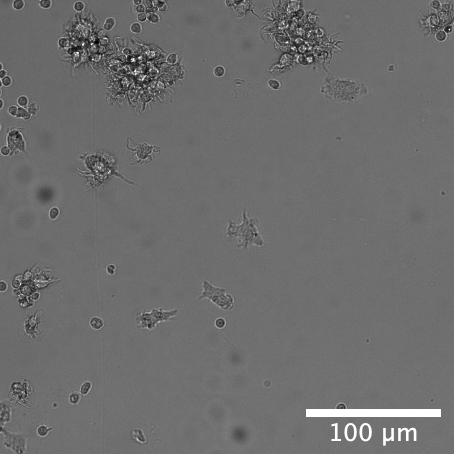
\includegraphics[width=\textwidth]{dissertation/figures/example_DCs_CK19O21.png}
    \end{subfigure}
    \begin{subfigure}[h!]{0.3\textwidth}
        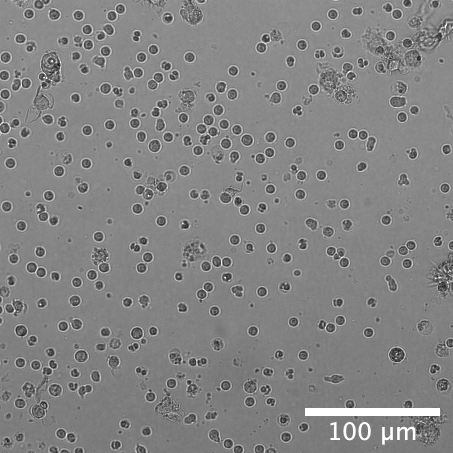
\includegraphics[width=\textwidth]{dissertation/figures/example_Tcells_CK22B12.png}
    \end{subfigure}
    \caption{Brightfield microscope images of dendritic cells (left) and T cells (right). Dendritic cells are named after their branching, tree-like structure. T cells are generally round.}
    \label{fig:real_cells}
\end{figure}

\begin{figure}[h]
    \centering
    \begin{subfigure}[h!]{0.3\textwidth}
        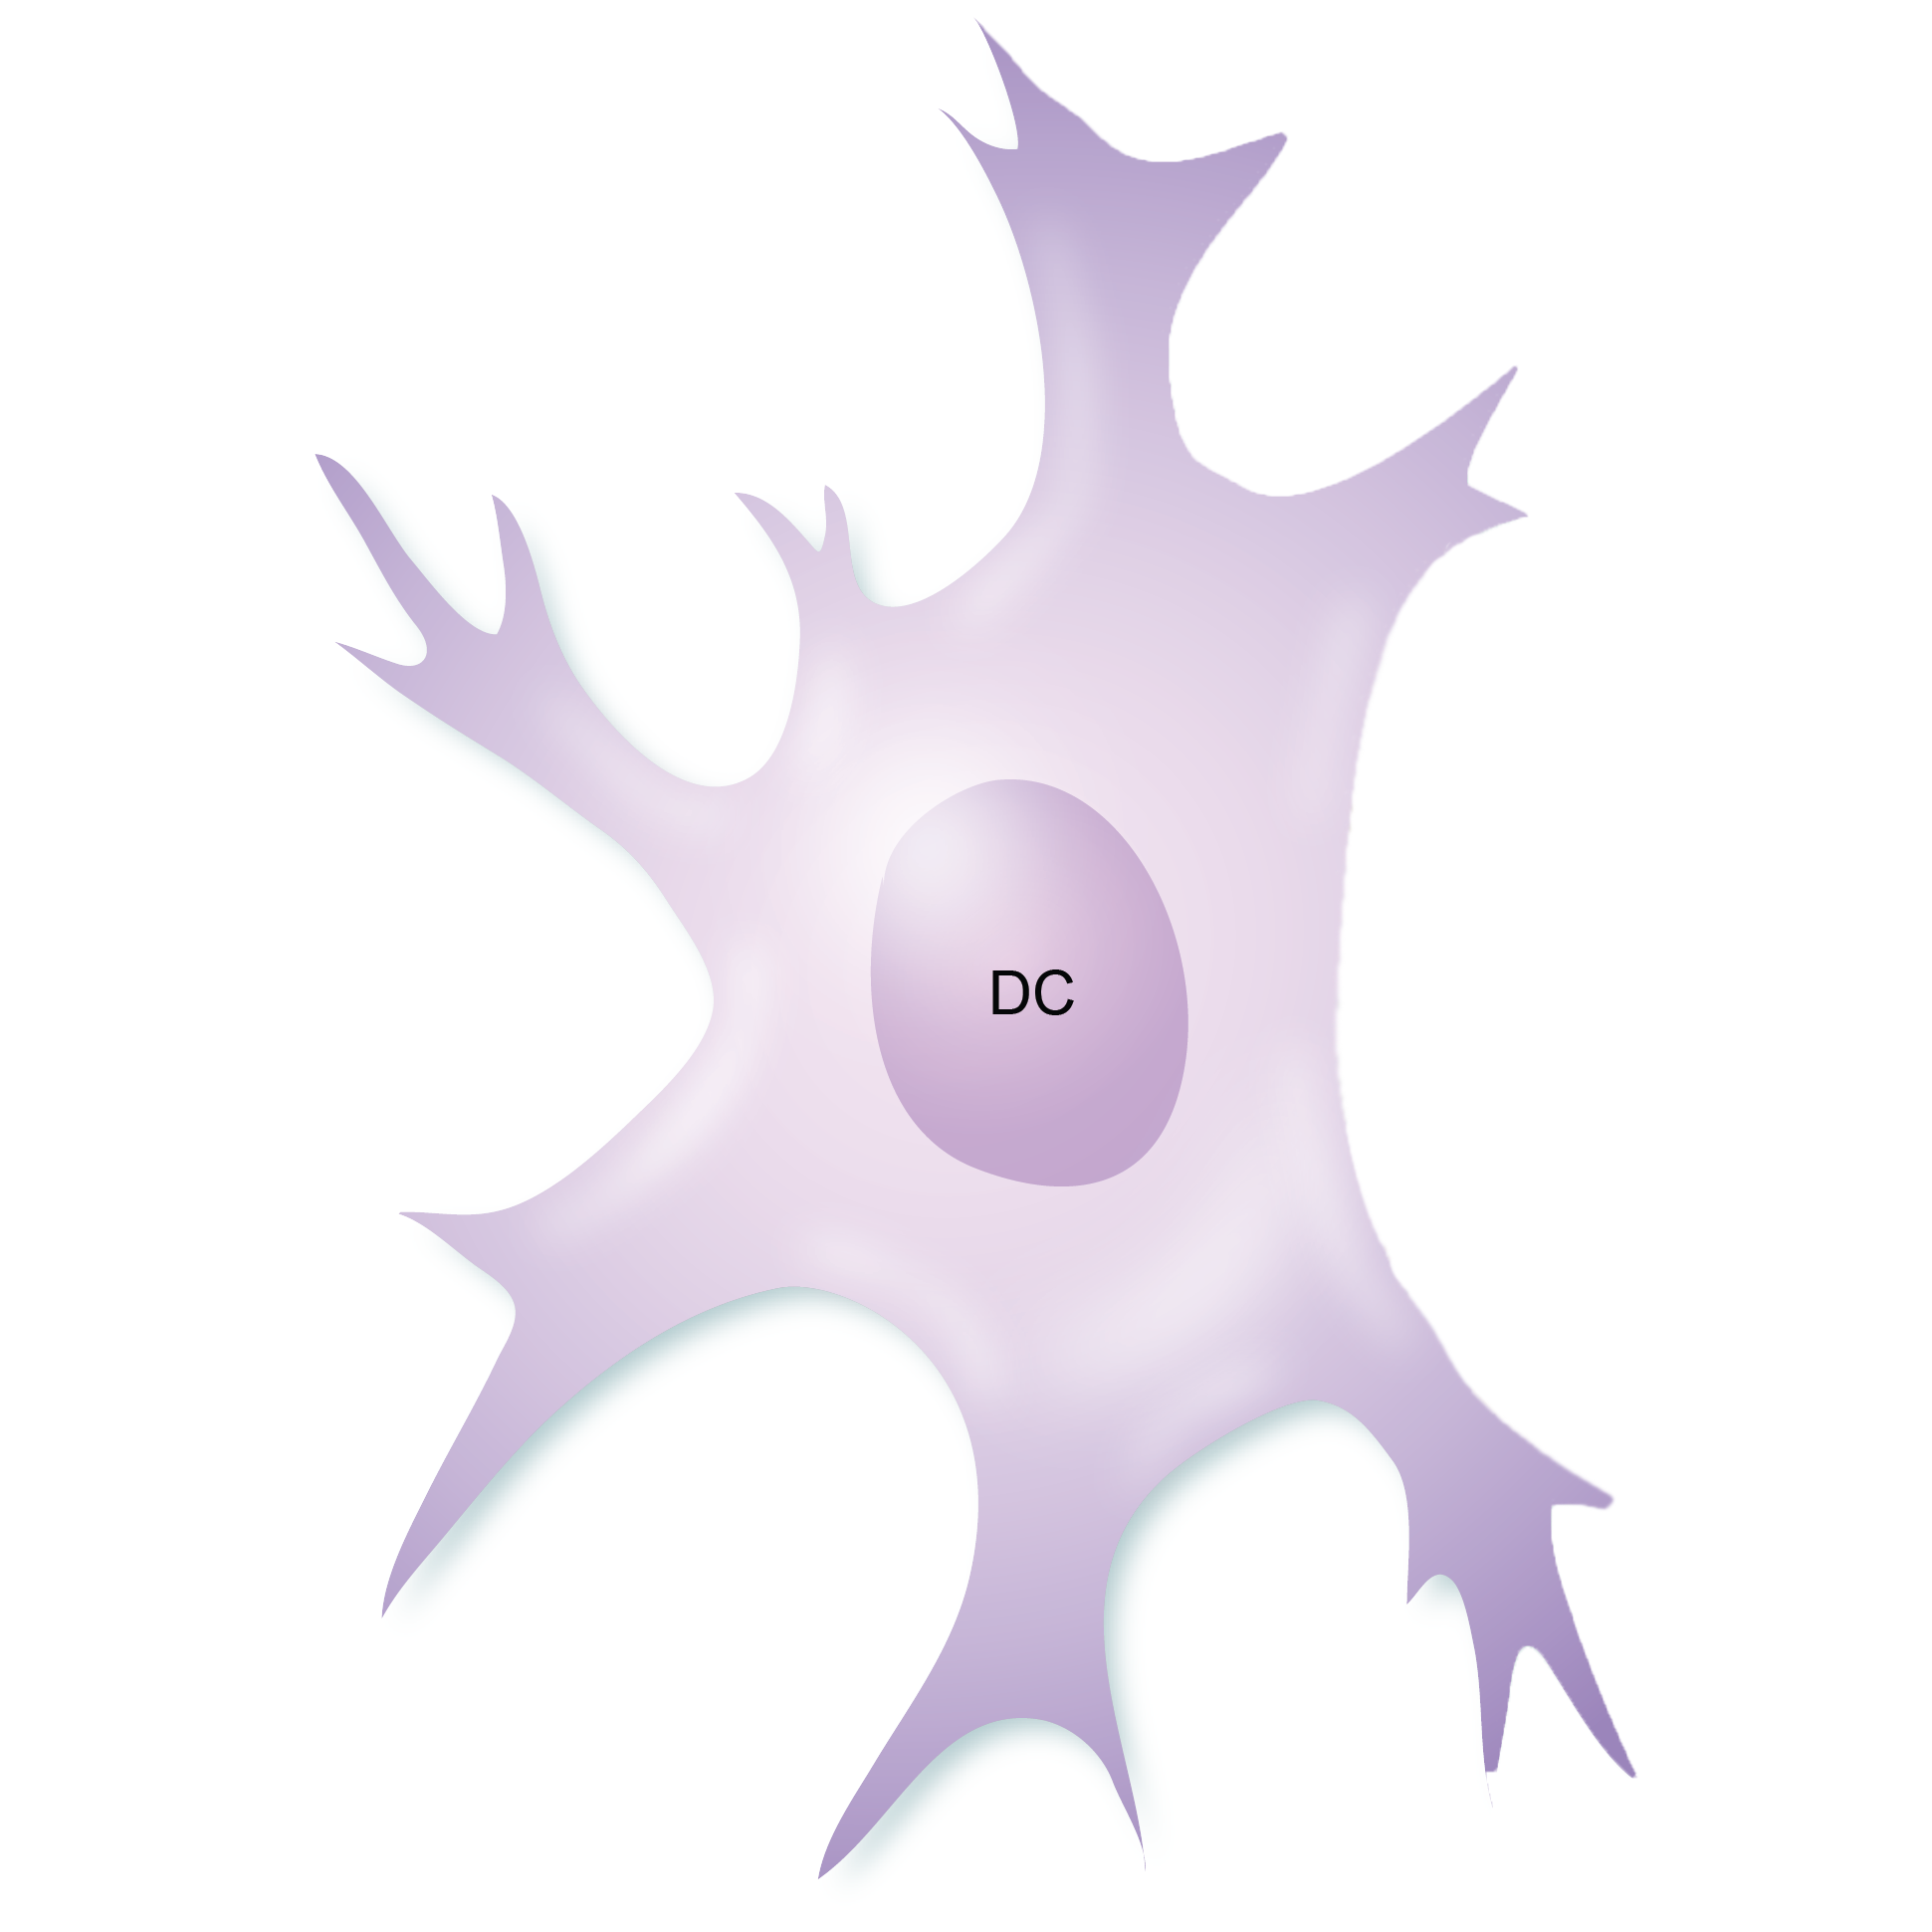
\includegraphics[width=\textwidth]{dissertation/figures/model_DC.png}
    \end{subfigure}
    \begin{subfigure}[h!]{0.3\textwidth}
        
\includegraphics[width=\textwidth]{dissertation/figures/model_Tcell.png}
    \end{subfigure}
    \caption{Schematic model of a dendritic cell (left) and a T cell (right), highlighting the tree-like structure of dendritic cells and the roundness of the shape of T cells. Adapted from \citet{cavanagh2020}}
    \label{fig:schematic_cells}
\end{figure}

The actors of our immune systems are thus the key defenders of our bodies. The actors we are interested in for the purpose of this research are T lymphocytes – ``T cells" – and dendritic cells – DCs (Figures \ref{fig:real_cells} and \ref{fig:schematic_cells}). Dendritic cells are ``sentinels" and initiate our immune system's responses by sensing and integrating information from their environment and sending it over to T cells. T cells are ``master controllers" and trigger the appropriate immune response, if any, from the information they have received, notably from dendritic cells, often in the form of chemical signals or intercellular interactions \citep{Brewster15, Rogh20}.

Antigens can be fought by antibodies, which are defensive proteins produced by our immune system. More specifically, antibodies are produced by B cells in a process which starts in T cells, and in some cases is activated by T cells seeing antigens on the surface of dendritic cells \citep{benson_antigen_2015}. B cells need the support of T cells to make highly effective antibodies. Hence, the interaction between dendritic cells and T cells is critical in the decision for our immune system to produce agents to defend our body.

The purpose of this dissertation is to evaluate how much interaction is observed between immune cells. There is existing work in the field of immunology looking into the effects of these changes in interaction. \citet{benson_antigen_2015} show how the generation of antibodies might be impacted by T cell and dendritic cell interaction. They studied how dendritic cells and T cells interacted in the mouse immune system, both in terms of whether or not interaction was witnessed, and of duration of interaction. This interaction was studied under different conditions, with different drug compounds being used to attempt to drive interaction or to inhibit it. They found that under conditions where compounds were blocking interaction between T cells and DCs, fewer antibodies were generated, meaning that the mice were not defending themselves as much. Hence, the study of the impact of compounds on the interactions between immune cells can tell us how our immune system will then operate. 

\subsection{Implications}

Concepts and research described in this section show that changes in interactions between immune cells control the way in which our immune system protects itself. Understanding how interactions react under the control of different drugs can give us targets for new therapies. Hence, analysing the interaction between immune cells under different experimental conditions bears a particular interest in the field of immunology for studying immune responses. We want to analyse this interaction with the help of deep learning techniques. 

\section{Concepts of interest in deep learning} \label{sec:deepl_bg}

The following sections collate selected research that show how deep learning techniques could be applied in the context of our study. 

\subsection{Convolutional operations for image feature extraction}

%A number of approaches already use deep neural networks for classification from textual genome sequences, particularly for cancer type detection (\cite{https://www.biorxiv.org/content/10.1101/612762v1}, \cite{https://www.nature.com/articles/s41598-019-53989-3}). 
Convolutional operations in neural networks were first introduced for pattern recognition by \citet{fukushima_neocognitron_1980}. They were later popularised by \citet{lecun_1989} as a method for object recognition, once back-propagation was put to use as a learning procedure for networks. LeCun applied his convolutional neural network (CNN) to digit recognition and subsequent classification and explored these networks in multiple papers. Since then, convolutional operations in neural networks have proven successful to extract features from more complex images. The AlexNet model published by \citet{krizhevsky_imagenet_2012} popularised the use of CNNs employing the acceleration of GPUs in computer vision. \citet{rawat_deep_2017} provide a comprehensive review of deep convolutional neural networks applied to the general task of image classification. In a recent medical example, \citet{shen_2019} trained a convolutional neural network structure to detect breast cancer from mammography screenings which showed competitive results compared to commercial systems. 

\subsection{Autoencoders for dimensionality reduction}

An autoencoder is a type of neural network trained to map its input to itself via a compressed representation of the input, as shown in Figure \ref{fig:autoencoder}. The compressed representation of the input obtained from the bottleneck layer is a \textit{coded} representation of the input, while the final output of the network is the \textit{decoded} version of the input. Autoencoders are not trained to learn a perfect copy of the input data, but a smaller, compressed copy with features which the neural network learns to be most important to be able to gain an overall understanding of the input. Autoencoders were first introduced in the 1980s \citep{rumelhart_1986} and are traditionally used for dimensionality reduction and feature extraction \citep{Goodfellow-et-al-2016}. 

\begin{figure}[h!]
    \centering
    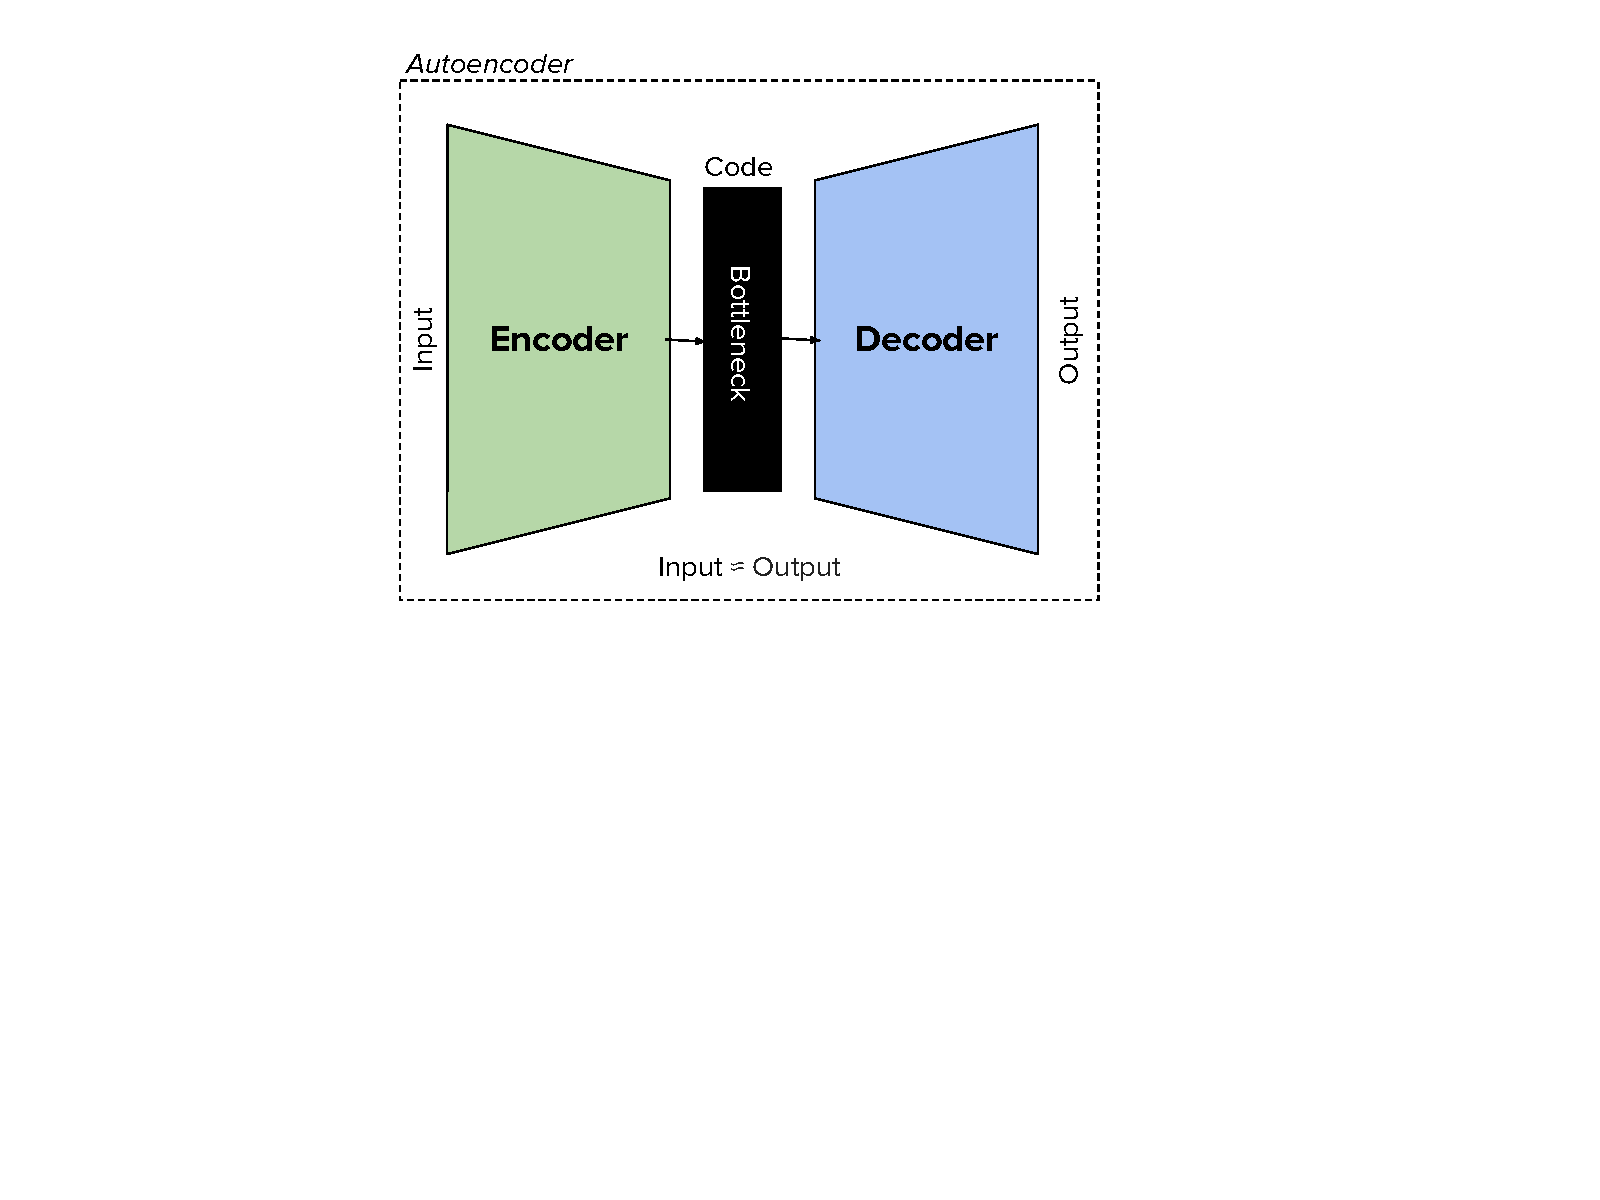
\includegraphics[width=0.45\textwidth]{dissertation/figures/autoencoder_schema.pdf}
    \caption{Schematic representation of an autoencoder. An autoencoder consists of two blocks of layers: encoding layers and decoding layers. The bottleneck layer holds a smaller representation of the input created by the encoder layer, from which we try to recreate the input in the decoder layers.}
    \label{fig:autoencoder}
\end{figure}

\citet{Zamparo2015} show that autoencoders can be successfully applied for dimensionality reduction in the context of biomedical data. Their autoencoder approach, applied to the unsupervised clustering of cell phenotypes, outperformed other dimensionality reduction techniques such as Principal Component Analysis. However, this approach was not applied to imaging data. Nonetheless, autoencoders have been successfully used for reducing the dimensionality of large imaging data by using convolution operations in their structure \citep{wang2016, saenz2018}.

\subsection{Deep regression models}

Neural networks can be constructed for regression tasks such that the model is trained to map from an input data, e.g. images, to real-values from a continuous range. \citet{Lathu2018} provide a review and comparison of common regression network architectures. In a medical example, both \citet{Xie15} and \citet{Xue2017} show promising results for using CNNs to extract numerical features from images of cell by using neural networks for the regression task of counting the number of cells in an image. 

\section{Finding structure in high-dimensional data} \label{sec:bg_visualisation}

The data we will be studying consists of images of cells obtained through high content screening (HCS). HCS is a method for capturing images of cells in multi-well plates, using high-resolution microscopy \citep{buchser_assay_2014}. A plate captured with high content screening can yield a large number of images in very high-resolution, typically around $2000\times2000$ pixels. This makes the analysis of the physical characteristics of a cell possible at a granular level. However, this also makes the dataset high-dimensional, which requires the use of visualisation techniques that map high-dimensional data points to a low-dimensional plane if we are looking to gauge the structure of the data. In this section we highlight two commonly used techniques for high-dimensional data visualisation.

\textbf{t-distributed stochastic neighbor embedding (t-SNE)} was developed in 2008 by \citeauthor{vanDerMaaten2008} as a technique to map high-dimensional data to two- or three-dimensional space. t-SNE can find structure in high-dimensional data by using the local relationships between data points and optimising results using gradient descent. These local relationships are defined using a Gaussian probability distribution in high dimensional space, and then recreated using the Student t-distribution. \citet{wattenberg2016how} provide a comprehensive guide on understanding the inner workings of t-SNE. 

\textbf{Uniform Manifold Approximation and Projection for Dimension Reduction (UMAP)} is a dimensionality reduction technique first published in 2018 by \citeauthor{umap_arxiv}. It has shown competitive results compared to t-SNE. UMAP works by constructing a high-dimensional weighted graph representation of the data. Each edge between points in the graph is weighted according to how likely the points are to be connected. UMAP transforms the high-dimensional graph representation into a low-dimensional representation that is as similar as possible, optimising results in the same way that t-SNE does. \citet{Coenon2019} provide a similar guide as for t-SNE above for grasping the inner workings of UMAP.

\begin{figure}[h]
    \centering
    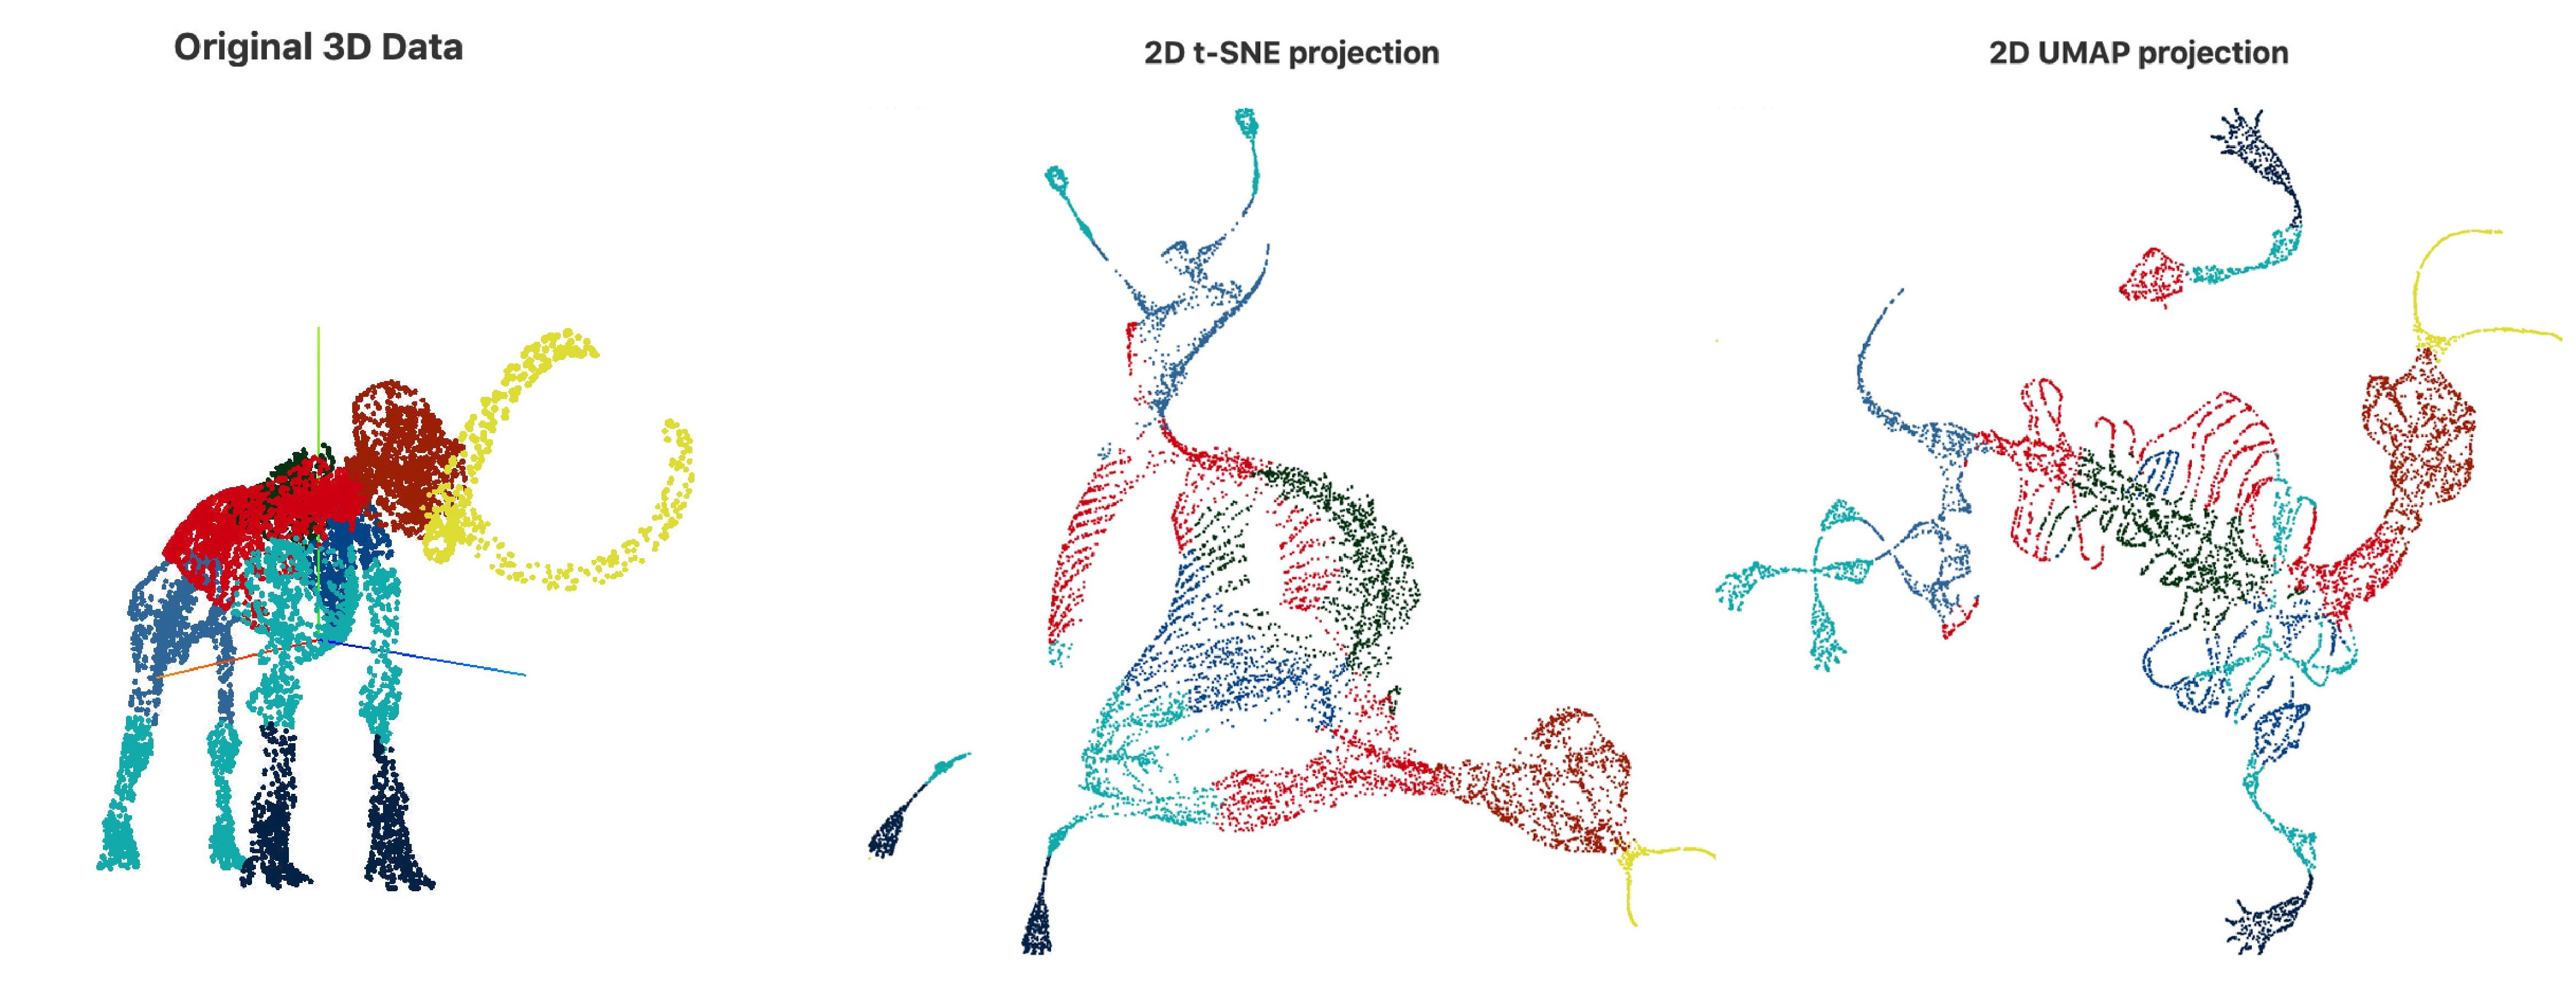
\includegraphics[width=\textwidth]{dissertation/figures/mammoth_vis.pdf}
    \caption{Three-dimensional model of a mammoth (left) projected to a two-dimensional plane with t-SNE (middle) and UMAP (right). t-SNE was applied with  $perplexity=2000$. UMAP was applied with $n\_neighbors=200$ and $min\_dist=0.25$. Source: \citet{Coenon2019}}
    \label{fig:vis_mammoth}
\end{figure}

The main differences between t-SNE and UMAP are of speed and parameters. The original UMAP paper compares UMAP's performance with t-SNE's on the MNIST digit dataset which consists of 70,000 $28\times28$ images of digits (0-9). On the researcher's 2017 MacBook Pro with i7 core and 8 GB of RAM, UMAP takes 87 seconds to run, while t-SNE takes 1,450 seconds \citep{umap_arxiv}.

t-SNE's main parameter to be tweaked is `perplexity', which loosely corresponds to an estimate of the number of neighbours each data point has \citep{wattenberg2016how}. UMAP's main parameters are number of neighbours and minimum distance. The former corresponds to the number of approximate neighbours a data point has, similar to t-SNE's perplexity. The latter corresponds to the minimum distance between points in low-dimensional space, meaning that it will tell UMAP how tightly to cluster points together, making visualisation more flexible.

The capabilities of t-SNE and UMAP are best illustrated through examples as shown in Figures \ref{fig:vis_mammoth} for a 3D to 2D projection and \ref{fig:vis_mnist} for a projection from higher high-dimensional points. It is important to note that in both techniques, distances between points in lower dimensions do not necessarily reflect their distances in higher dimensions \citep{Coenon2019}.

\begin{figure}[!ht]
    \centering
    \begin{subfigure}{.45\textwidth}
        \includegraphics[width=\textwidth]{dissertation/figures/mnist_tsne.png}
        \caption{t-SNE projection}
    \end{subfigure}
    \begin{subfigure}{.45\textwidth}
        \includegraphics[width=\textwidth]{dissertation/figures/mnist_umap.png}
        \caption{UMAP projection}
    \end{subfigure}
    \caption{70,000 points of the MNIST digit dataset images projected to a two-dimensional plane with t-SNE (left) and UMAP (right). t-SNE was applied with its default parameters and $perplexity=30$. UMAP was applied with $n\_neighbors=50$ and $min\_dist=0.65$ to have clusters of similar sizes as t-SNE. Each point corresponds to the image of a handwritten digit. We can see that same-digits are generally clustered together with both techniques.}
    \label{fig:vis_mnist}
\end{figure}

In the case of our research, applying t-SNE or UMAP to a dataset of microscope image could allow us to uncover whether or not immune cells behave in recognisable ways under different experimental conditions and whether or not this can be recognised from the structure of the images.

\section{The place of deep learning in immunology} \label{sec:dl_immunology}

A quantity of existing research already uses broader machine learning (ML) techniques in the field of immunology. \citet{muh_allerhunter_2009} applied Support Vector Machines (SVMs) to the study of allerginicity. Allergic reactions are triggered when the immune system wrongly assumes a harmless substance to be dangerous, such as dust, and produces antibodies to attack it \citep{tregoning2020}. The SVMs were used to analyse the DNA sequences of known allergens and known non-allergens. The aim was to try and make accurate predictions on previously unseen sequences and classify them as either allergenic or non-allergenic. The model achieved 95.3\% accuracy.  In another classification example, \citet{david_using_2010} used a Bayesian classifier and a decision tree to predict the likelihood of degenerative disorders from the sequencing of antibodies and achieved a best accuracy score of 89\%. 

The above examples represent examples of immunology research carried out using traditional ML techniques. Emerging deep learning research on cell imaging data now additionally includes cell segmentation \citep{al-kofahi_deep_2018}. In cancer research, deep neural networks are increasingly being used for feature extraction from images to accurately detect cancer \citep{litjens_deep_2016, bychkov_deep_2018}. Research specifically using immune cell data is mostly focused on cell counting \citep{turkki_antibody-supervised_2016, aprupe_robust_2019}. 

\section{Summary}

The research presented and cited here highlights that there is an increasing array of methods available to process high-dimensional, visual data through deep learning and visualisation techniques. This section has shown that immunology researchers have successfully made use of machine learning techniques, and that immunology-related fields such as cancer research have successfully applied deep learning methods in their research to obtain promising results. There is indeed an increasing interest in the applications of deep learning in medical fields, but the use of deep neural networks has not been fully explored in the context of studying immune cells interactions. There seems to be a lack of research into the qualitative and quantitative analysis of immune cell interactions from imaging data through deep learning. However and as shown above, immune cell interactions are of particular interest in drug research as they are key in understanding how an immune system operates.

This dissertation will focus on filling this gap, applying deep learning to extract features from images of immune cells in order to generate qualitative or quantitative data about the interactions between T cells and dendritic cells under different experimental conditions.
\chapter{Materials and Methods} \label{sec:mm}

This chapter covers the images that were available for analysis, how they were processed, and which methods were applied to analyse them. Detailed results of the implementation of these methods are then presented and discussed in Section \ref{sec:implementation}.

\section{Immune cells dataset}

\subsection{Setup}

The images that were used for the purpose of this research were provided by the Laboratory of Immune Cell Visualisation and Examination (LIVE) at the Institute of Infection, Immunity \& Inflammation at the University of Glasgow. The images are captured from 384-well plates with a commercial INCell Analyzer 2000. As established in Section \ref{bg:immunesystem}, the type of immune cells we are studying are T cells and dendritic cells (DCs). Each plate to be imaged in the INCell Analyzer contains a grid of wells as shown in Figure \ref{fig:384_well}. Each of those wells is assigned a label and an experimental condition. T cells, dendritic cells, and compounds related to the experimental conditions are injected in the well. In order to be able to distinguish between them, cells are loaded with fluorescent dyes: the T cells are dyed with a green dye (CSFE dye), and the dendritic cells are dyed with a red dye (CMTPX dye). After imaging, we obtain three field-of-view images per well: 

\begin{itemize}
    \item a Brightfield image, which shows both T cells and dendritic cells (Figure \ref{fig:fov_brightfield})
    \item an image showing only the T cells, which has been captured through the fluorescent green dye (Figure \ref{fig:fov_fitc})
    \item an image showing only the dendritic cells, which has been captured through the fluorescent red dye (Figure \ref{fig:fov_tr}).
\end{itemize}

\begin{figure}[h]
    \centering
    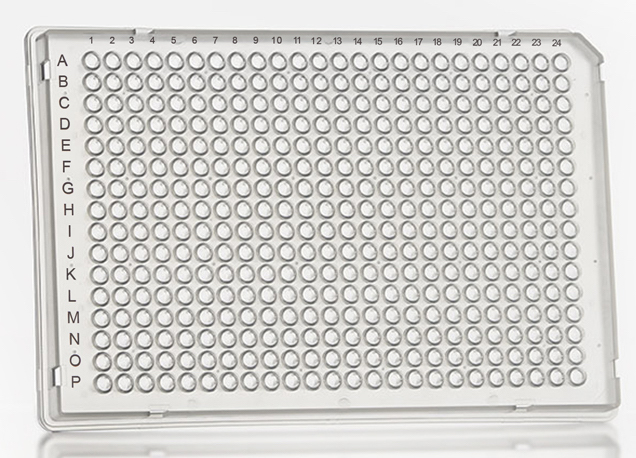
\includegraphics[width=.4\textwidth]{dissertation/figures/384_well.jpg}
    \caption{Example of a 384-well plate. Each well is labelled by a letter (vertically) and a number (horizontally). Source: Brooks Life Sciences.}
    \label{fig:384_well}
\end{figure}

\begin{figure}[h]!
    \centering
    \begin{subfigure}[h!]{0.3\textwidth}
        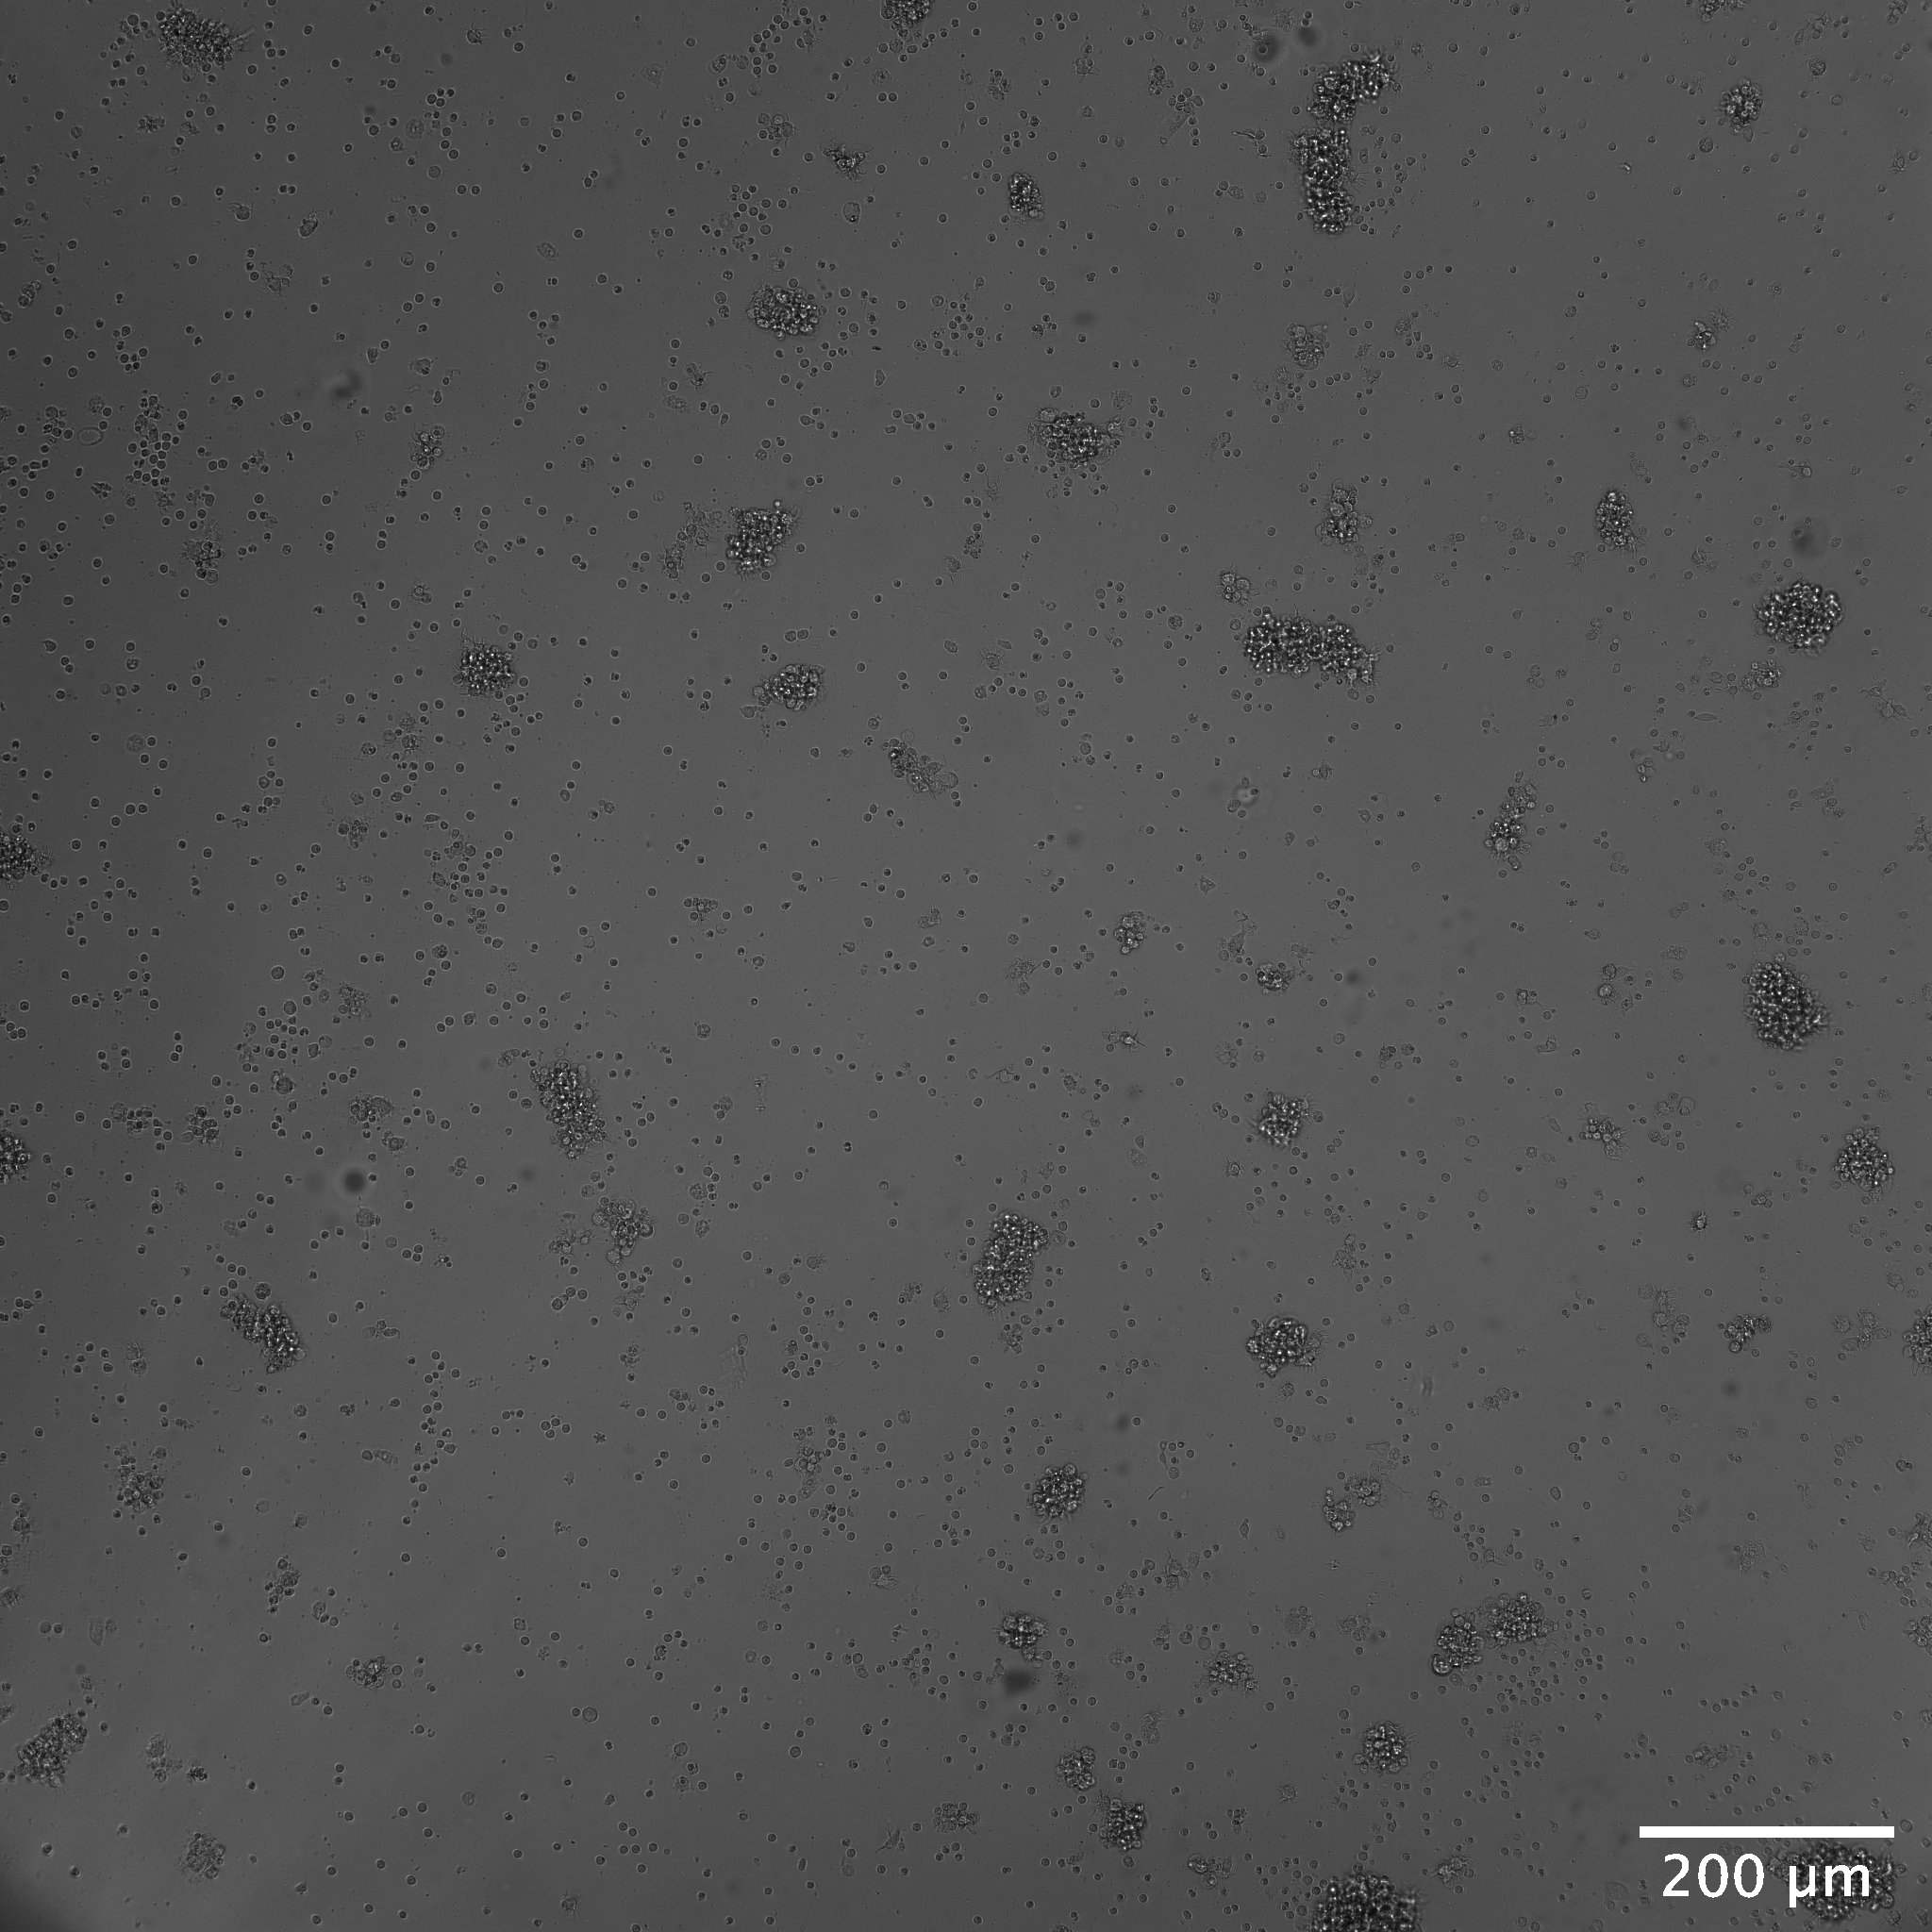
\includegraphics[width=\textwidth]{dissertation/figures/example_Brightfield_L20.jpg}
        \caption{Brightfield view}
        \label{fig:fov_brightfield}
    \end{subfigure}
    \begin{subfigure}[h!]{0.3\textwidth}
        
\includegraphics[width=\textwidth]{dissertation/figures/example_FITC_L20.png}
        \caption{Green dye (T cells) view}
        \label{fig:fov_fitc}
    \end{subfigure}
    \begin{subfigure}[h!]{0.3\textwidth}
        \includegraphics[width=\textwidth]{dissertation/figures/example_TexasRed_L20.png}
        \caption{Red dye (DCs) view}
        \label{fig:fov_tr}
    \end{subfigure}
    \caption{Microscope images extracted from the dataset showing each view obtained with the capture system. Brightness has been adjusted for \subref{fig:fov_fitc}, \subref{fig:fov_tr} for details to come through.}
    \label{fig:fov}
\end{figure}

\subsection{Experimental conditions}

Approximately 8,000 dendritic cells and 8,000 T cells were cultured in each of the 384 wells. The INCell Analyzer 2000 captured an image of 25\% of each well. The dendritic cells were cultured from bone marrow cells obtained from mice. T cells were obtained from mouse lymphoid tissues. About 70 to 90\% of mouse T cells expressed a receptor for the Ovalbumin (OVA) peptide antigen, which means they recognised it well. 

Each well in a plate was associated with an experimental condition:
\begin{itemize}
    \item The well are injected with one of 45 drug compounds, 
    \item These compounds could be injected at a bigger or lesser concentration,
    \item Moreover, one of two types of antigens could be supplemented to further stimulate the cells. 
\end{itemize}

We were interested in using the latter as a label for our images, as it gives us a smaller number of categories to look at. More specifically, there are three categories of stimulation: 
\begin{itemize}
    \item No stimulation
    \item Stimulation with Ovalbumin (OVA) peptide, which is the antigen that should be recognised by most T cells in the well
    \item Stimulation with Concanavalin A (ConA), an antigen which cross-links T cells receptors with a molecule on the surface of DCs that would hold the OVA peptide antigen and present it to T cells
\end{itemize}

\subsection{Image selection} \label{subsec:selecting_dataset}

There was a large amount of images available from different well plates with the different experimental conditions described above. However, each set of images corresponding to a plate represents about 8 GB of data on average. Moving images through disks or cloud filing system thus represented substantial time and was vulnerable to transfer errors. Hence, a limited number of plates were selected for training and evaluation to make sure their consistency could be validated. Chosen plates were selected to best represent the experimental conditions were chosen for study, and were assigned to three datasets.

\begin{itemize}
    \item \textbf{The `full' dataset}: this dataset contained an equal number of images in the three categories of stimulation: no stimulation, stimulation with OVA, and simulation with ConA. This was to prevent issues of class imbalance when training the model. 
    \item \textbf{The simpler `dual' dataset}, with two categories: this dataset contained an equal number of images in two categories: no stimulation, and stimulation with OVA peptide. This was selected under the hypothesis that if useful results cannot be obtained with a dataset containing images from all categories, a deep learning model might be able to perform better with two categories. 
    \item \textbf{The `DMSO-only' dataset}: Dimethyl sulfoxide (DMSO) is a solvent that helps solubilise the investigated drug compounds, as most compounds are not initially water soluble. When in solution, drug compounds should be more bioavailable and have more of a biological impact. DMSO images in the original dataset only included DMSO and no drugs, and were used as a control. However, images of this dataset should show the most difference between stimulation categories as immune cells have not been impacted by drugs.
\end{itemize}

These datasets and characteristics are summarised in Table \ref{table:datasets}.

\begin{table}[h]
\centering
\caption{Number of images in each category of stimulation for each of the three datasets. Both full and dual datasets should have no issues with category imbalance.}
\begin{tabular}{|l|r|r|r|}
\rowcolor[HTML]{EFEFEF} 
\hline
Dataset & Unstimulated & OVA & ConA \\ \hline
Full    & 9,800        & 9,800 & 9,800    \\
Dual    & 6,900        & 6,900 & 0    \\
DMSO    & 4,000        & 2,000   & 2,000   \\ \hline
\end{tabular}
\label{table:datasets}
\end{table}

\subsection{Pre-processing} \label{subsec:preproc}
The datasets obtained from this setup consisted of $2048\times2048$ 16-bit images in TIFF format, captured by a 12-bit camera. As mentioned above, each ``image” consists of a set of three views: the green fluorescent image (T cells), the red fluorescent image (dendritic cells), and the brightfield image. The brightfield images show both cell types and can be used for diagnostic purposes when deciding on pre-processing methods, but were otherwise discarded and not used for further analysis.

Each of the images was about 8 MB in size, representing 4,194,304 pixels. This raised the issue of very high dimensions to handle for a model. Moreover, each plate had 384 wells, which corresponds to a total of about 800 images when counting both the T cells image and the DCs image. This meant that we had quite a limited amount of images to feed into any kind of model. 

Moreover, as shown on Figures \ref{fig:fov_fitc} and \ref{fig:fov_tr}, the smaller white dots of immune cells could easily be confused for dust on the screen, even to the naked eye. This could be as confusing for a deep learning model trying to learn features from an image as it could be for us. Furthermore, the issue of images being of very high dimensions remained. Indeed, a basic autoencoder with three $2\times2$ downsampling operations would yield around 500,000 pixel points from a $2048\times2048$ input image, which is still a very high number for a visualisation technique like t-SNE or UMAP. 

\bigskip
\subsubsection{Sliding window}    

\hfill\\
\hfill\\
To resolve this issue, the first idea was to make the images more manageable by a neural network by cropping a set square subsection of the image of smaller dimensions, for example a square of $250\times250$ pixels. However, this left the issue of having only limited input to train a neural network. Instead, images were pre-processed by passing a sliding window over the image, creating patches of images per file. This quickly expanded the size of the dataset, making it as large as 58,000 samples in some cases. Smaller images also made more sense to the naked eye, hence we assumed that a trained neural network would perform better on this gridded dataset than on a full-image dataset. 

\bigskip
\subsubsection{Normalisation}

\hfill\\
\hfill\\
Each sub-image was normalised with min-max normalisation (\autoref{equation:minmax}) to get a [0, 1] range of pixel values. It is common to normalise imaging data to the floating-point [0, 1] range over keeping an integer representation of an image, as integers are subject to saturation and rounding error. We used min-max normalisation as not all images in our dataset had 0 as their minimum value.  

\begin{equation}
    minmax(x) = \frac{x - min(x)}{max(x) - min(x)}
\label{equation:minmax}
\end{equation} 

\bigskip
\subsubsection{Noise and outlier detection}

\hfill\\
\hfill\\
From analysing the images, it was also found that some images contained many pixels in the range of [0, 255] before normalisation. Moreover, such pixels usually seemed to correspond to background noise as shown in Figure \ref{fig:bgnoise}. The fact that these lie in the range of an 8-bit image pixel range could be coincidental, or the result of the way the imaging system picked up non-stained elements in the well. The immunology researcher providing the images confirmed that this noise was present in some images read from specific plates. Wells in early experiments were injected with additional cells as researchers thought this made the cells behave more naturally, however this was later found to have no real impact. These cells were not stained by dyes, but some of their details still came through the imaging system. Although this background was not always visible to the naked eye, we did not want those pixel values to confuse a neural network model. Hence, values below 255 in images were clipped to 255 before min-max normalisation was applied.

\begin{figure}[h!]
    \centering
    \begin{subfigure}[h!]{0.99\textwidth}
        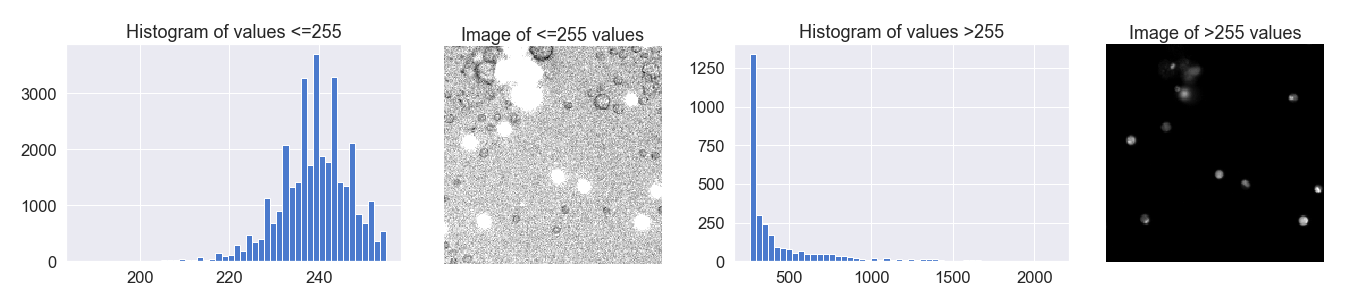
\includegraphics[width=\textwidth]{dissertation/figures/background_noise_true.png}
        \caption{Histogram and image analysis for a sub-image with noisy cells in the background}
        \label{fig:bgnoisetrue}
    \end{subfigure}
    
    \begin{subfigure}[h!]{0.99\textwidth}
        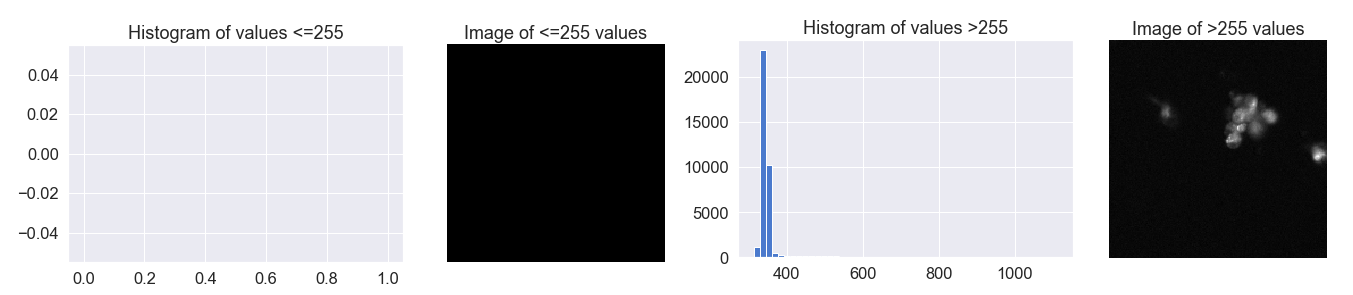
\includegraphics[width=\textwidth]{dissertation/figures/background_noise_false.png}
        \caption{Histogram and image analysis for a sub-image with no noisy cells in the background}
        \label{fig:bgnoisefalse}
    \end{subfigure}
    
    \caption{Histogram and image analysis for background noise detection}
    \label{fig:bgnoise}
    
\end{figure}

As described above, the provided images sometimes contained some background noise. Furthermore, some images contained larger amounts of noise coming from defects in the wells, such as water droplets. This is illustrated in Figure \ref{fig:noisyimage}. Their pixel value distribution followed the [0, 255] range as described above, but these values also covered the whole sub-image and no cells of interest were present in those patches. Removing them entirely from the dataset would have made it more difficult to rationalise the analysis of whole images. Indeed, by pre-processing full images with a sliding window, each full image is represented by a patch of a set number of sub-images. This would have created inconsistencies in the amount of sub-images per image file. Instead of removing them, it was decided to keep them in to evaluate if a neural network could make sense of them as a category. Noisy sub-images were labelled as ``Faulty". 

\begin{figure}[h!]
    \centering
    \begin{subfigure}[h!]{0.3\textwidth}
        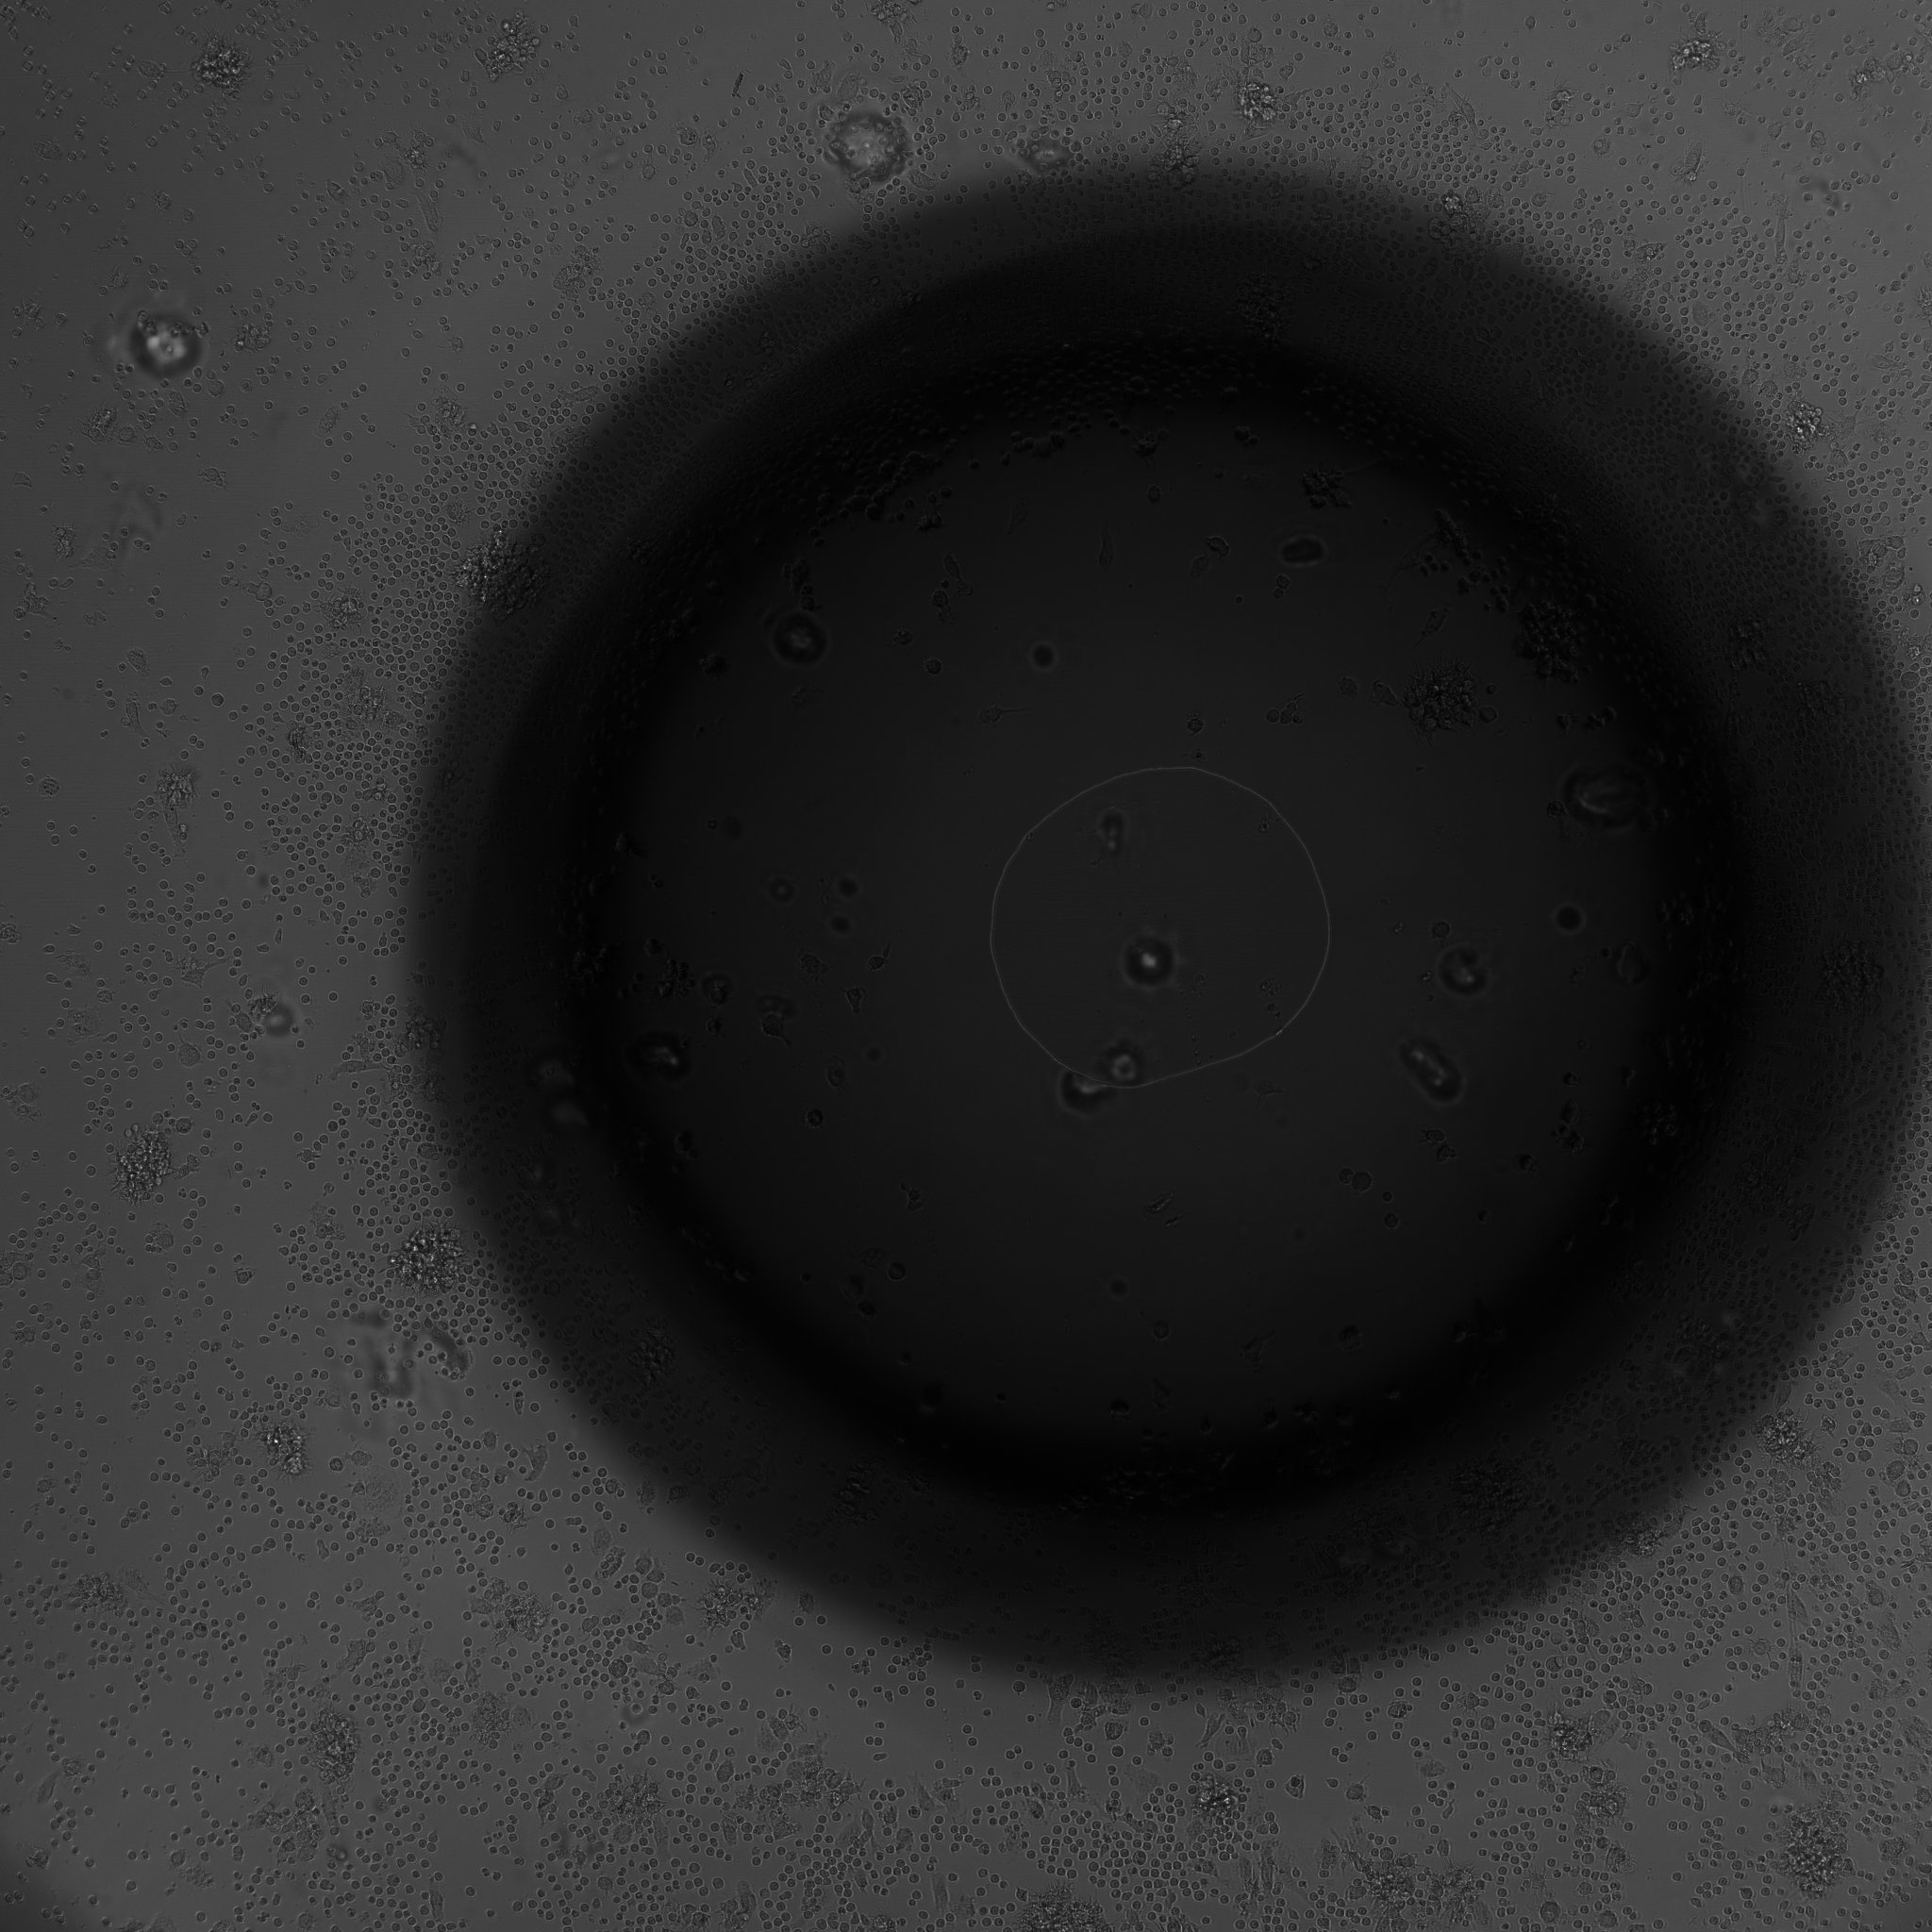
\includegraphics[width=\textwidth]{dissertation/figures/faulty_brightfield.jpg}
        \caption{Brightfield view}
    \end{subfigure}
    \begin{subfigure}[h!]{0.3\textwidth}
        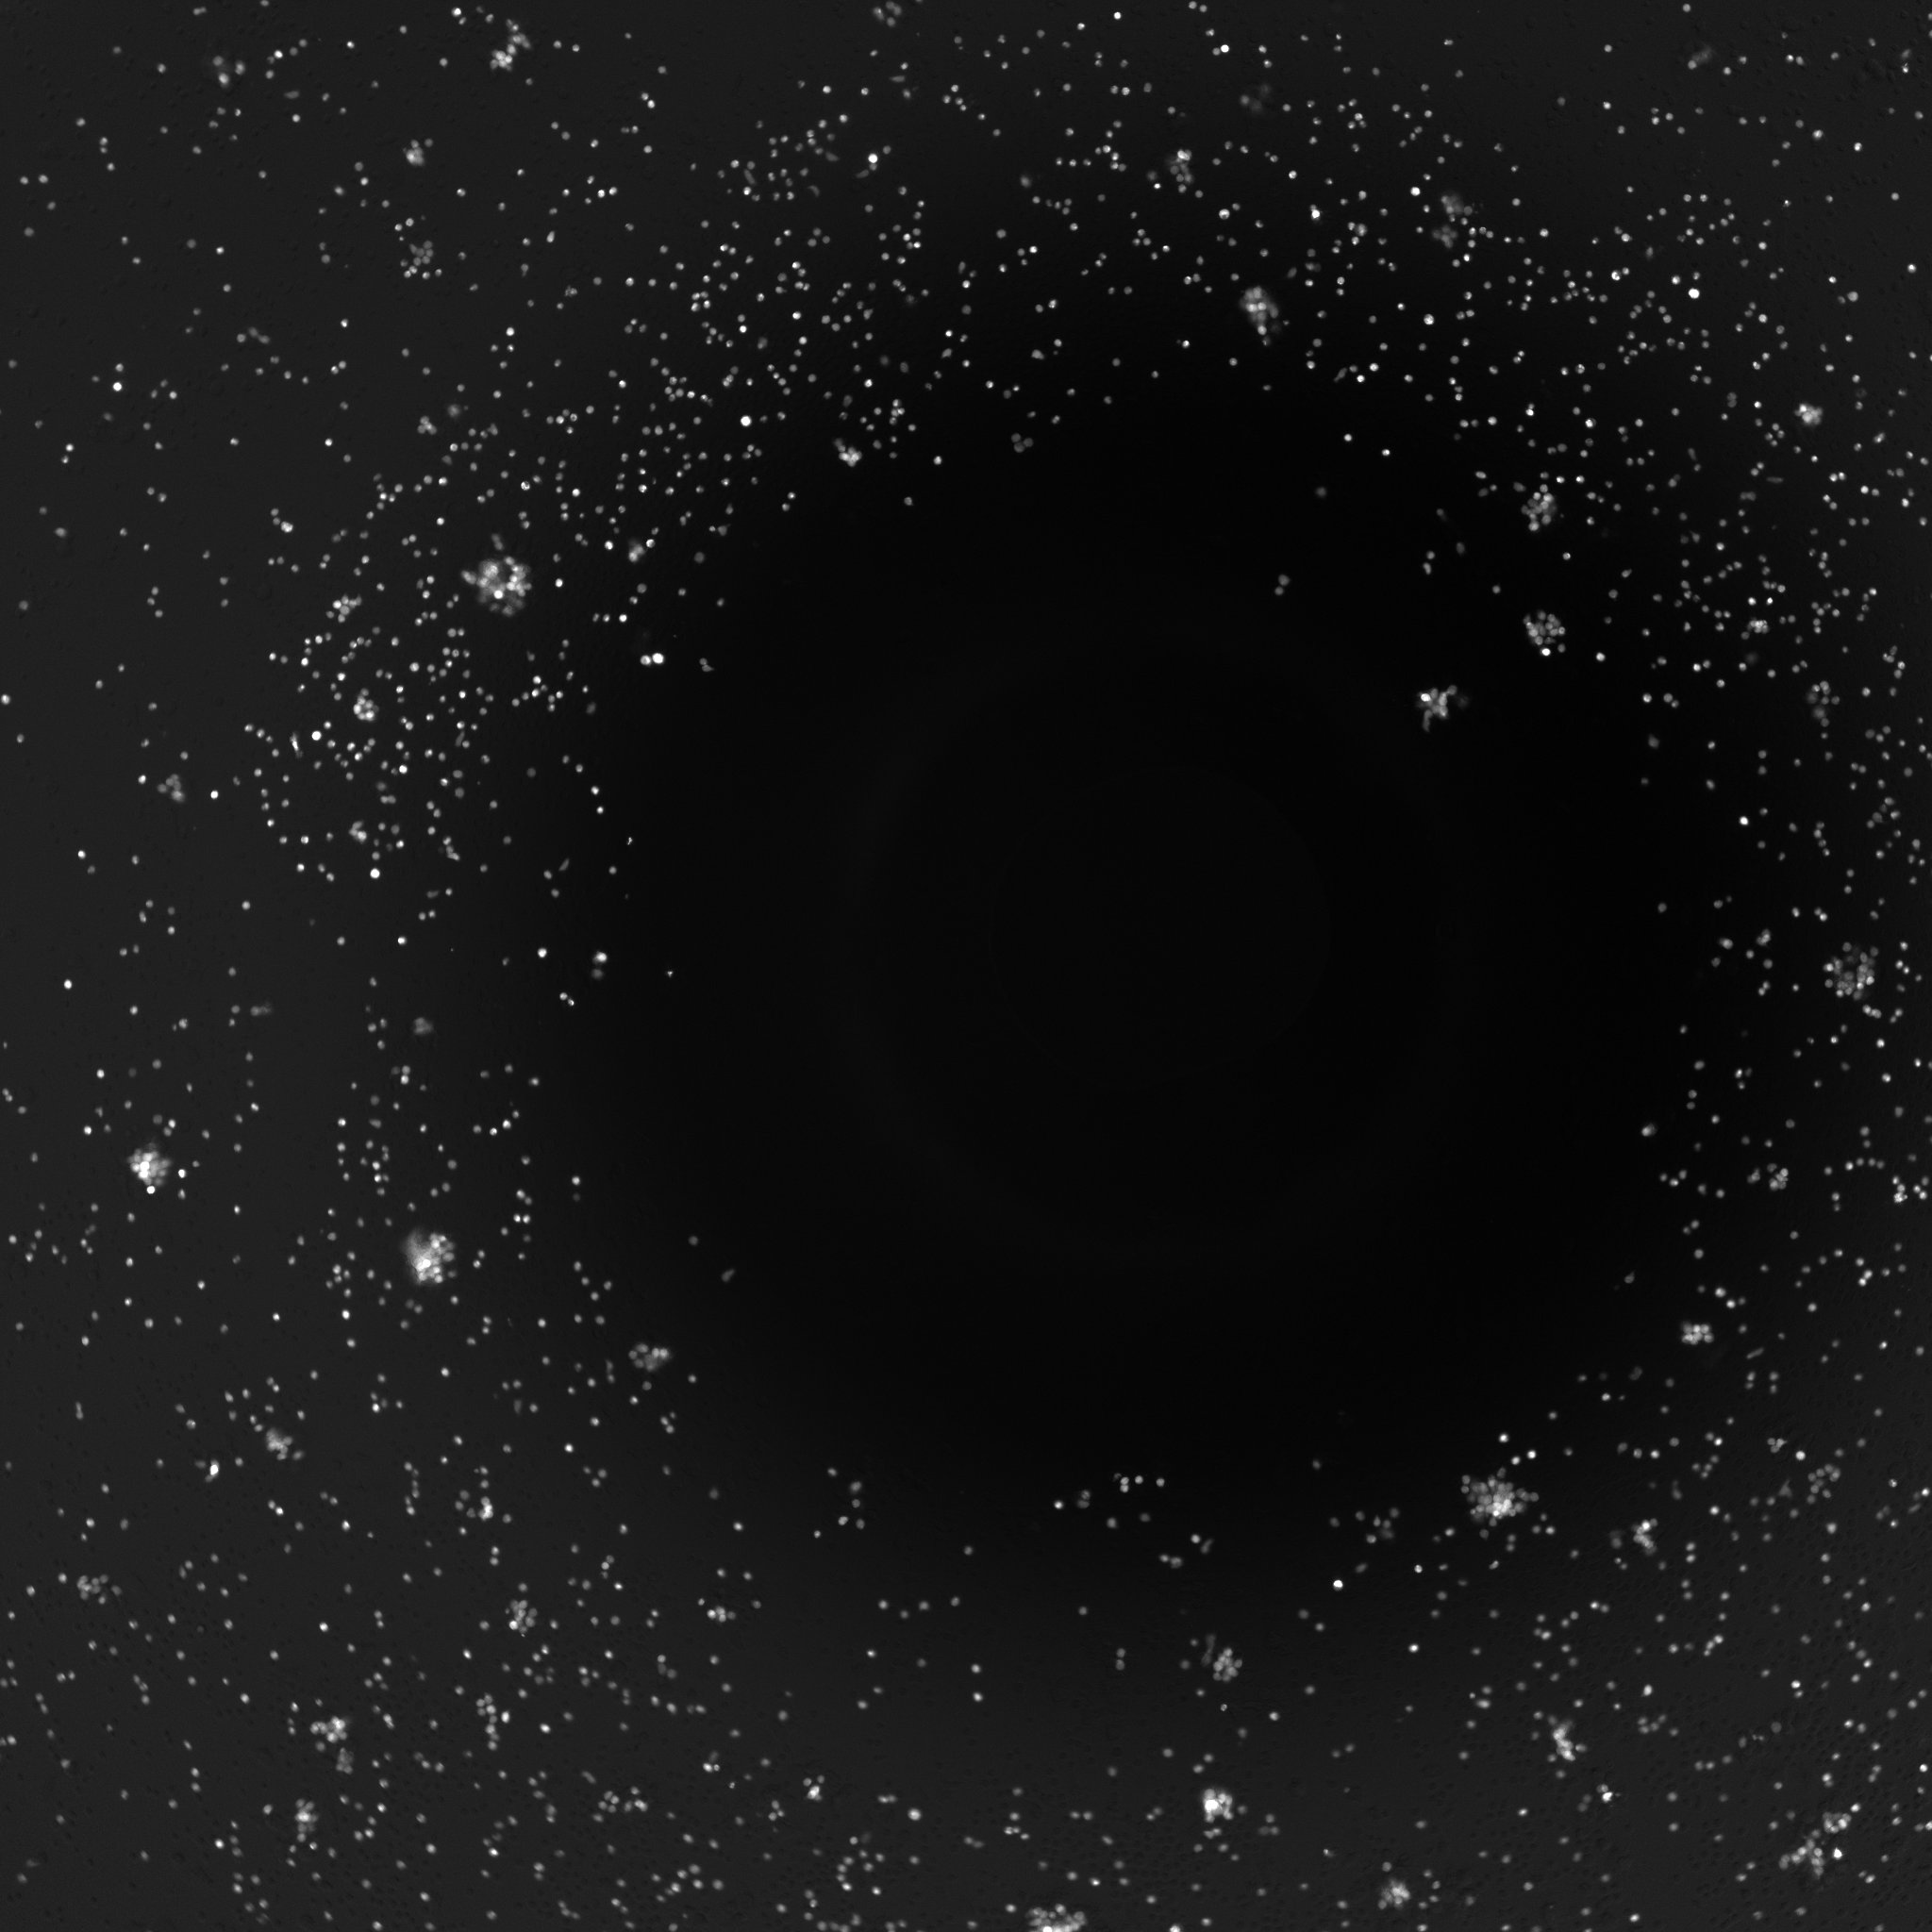
\includegraphics[width=\textwidth]{dissertation/figures/faulty_tcell.jpg}
        \caption{Green dye (T cells) view}
        \label{subfig:tcell}
    \end{subfigure}
    \begin{subfigure}[h!]{0.3\textwidth}
        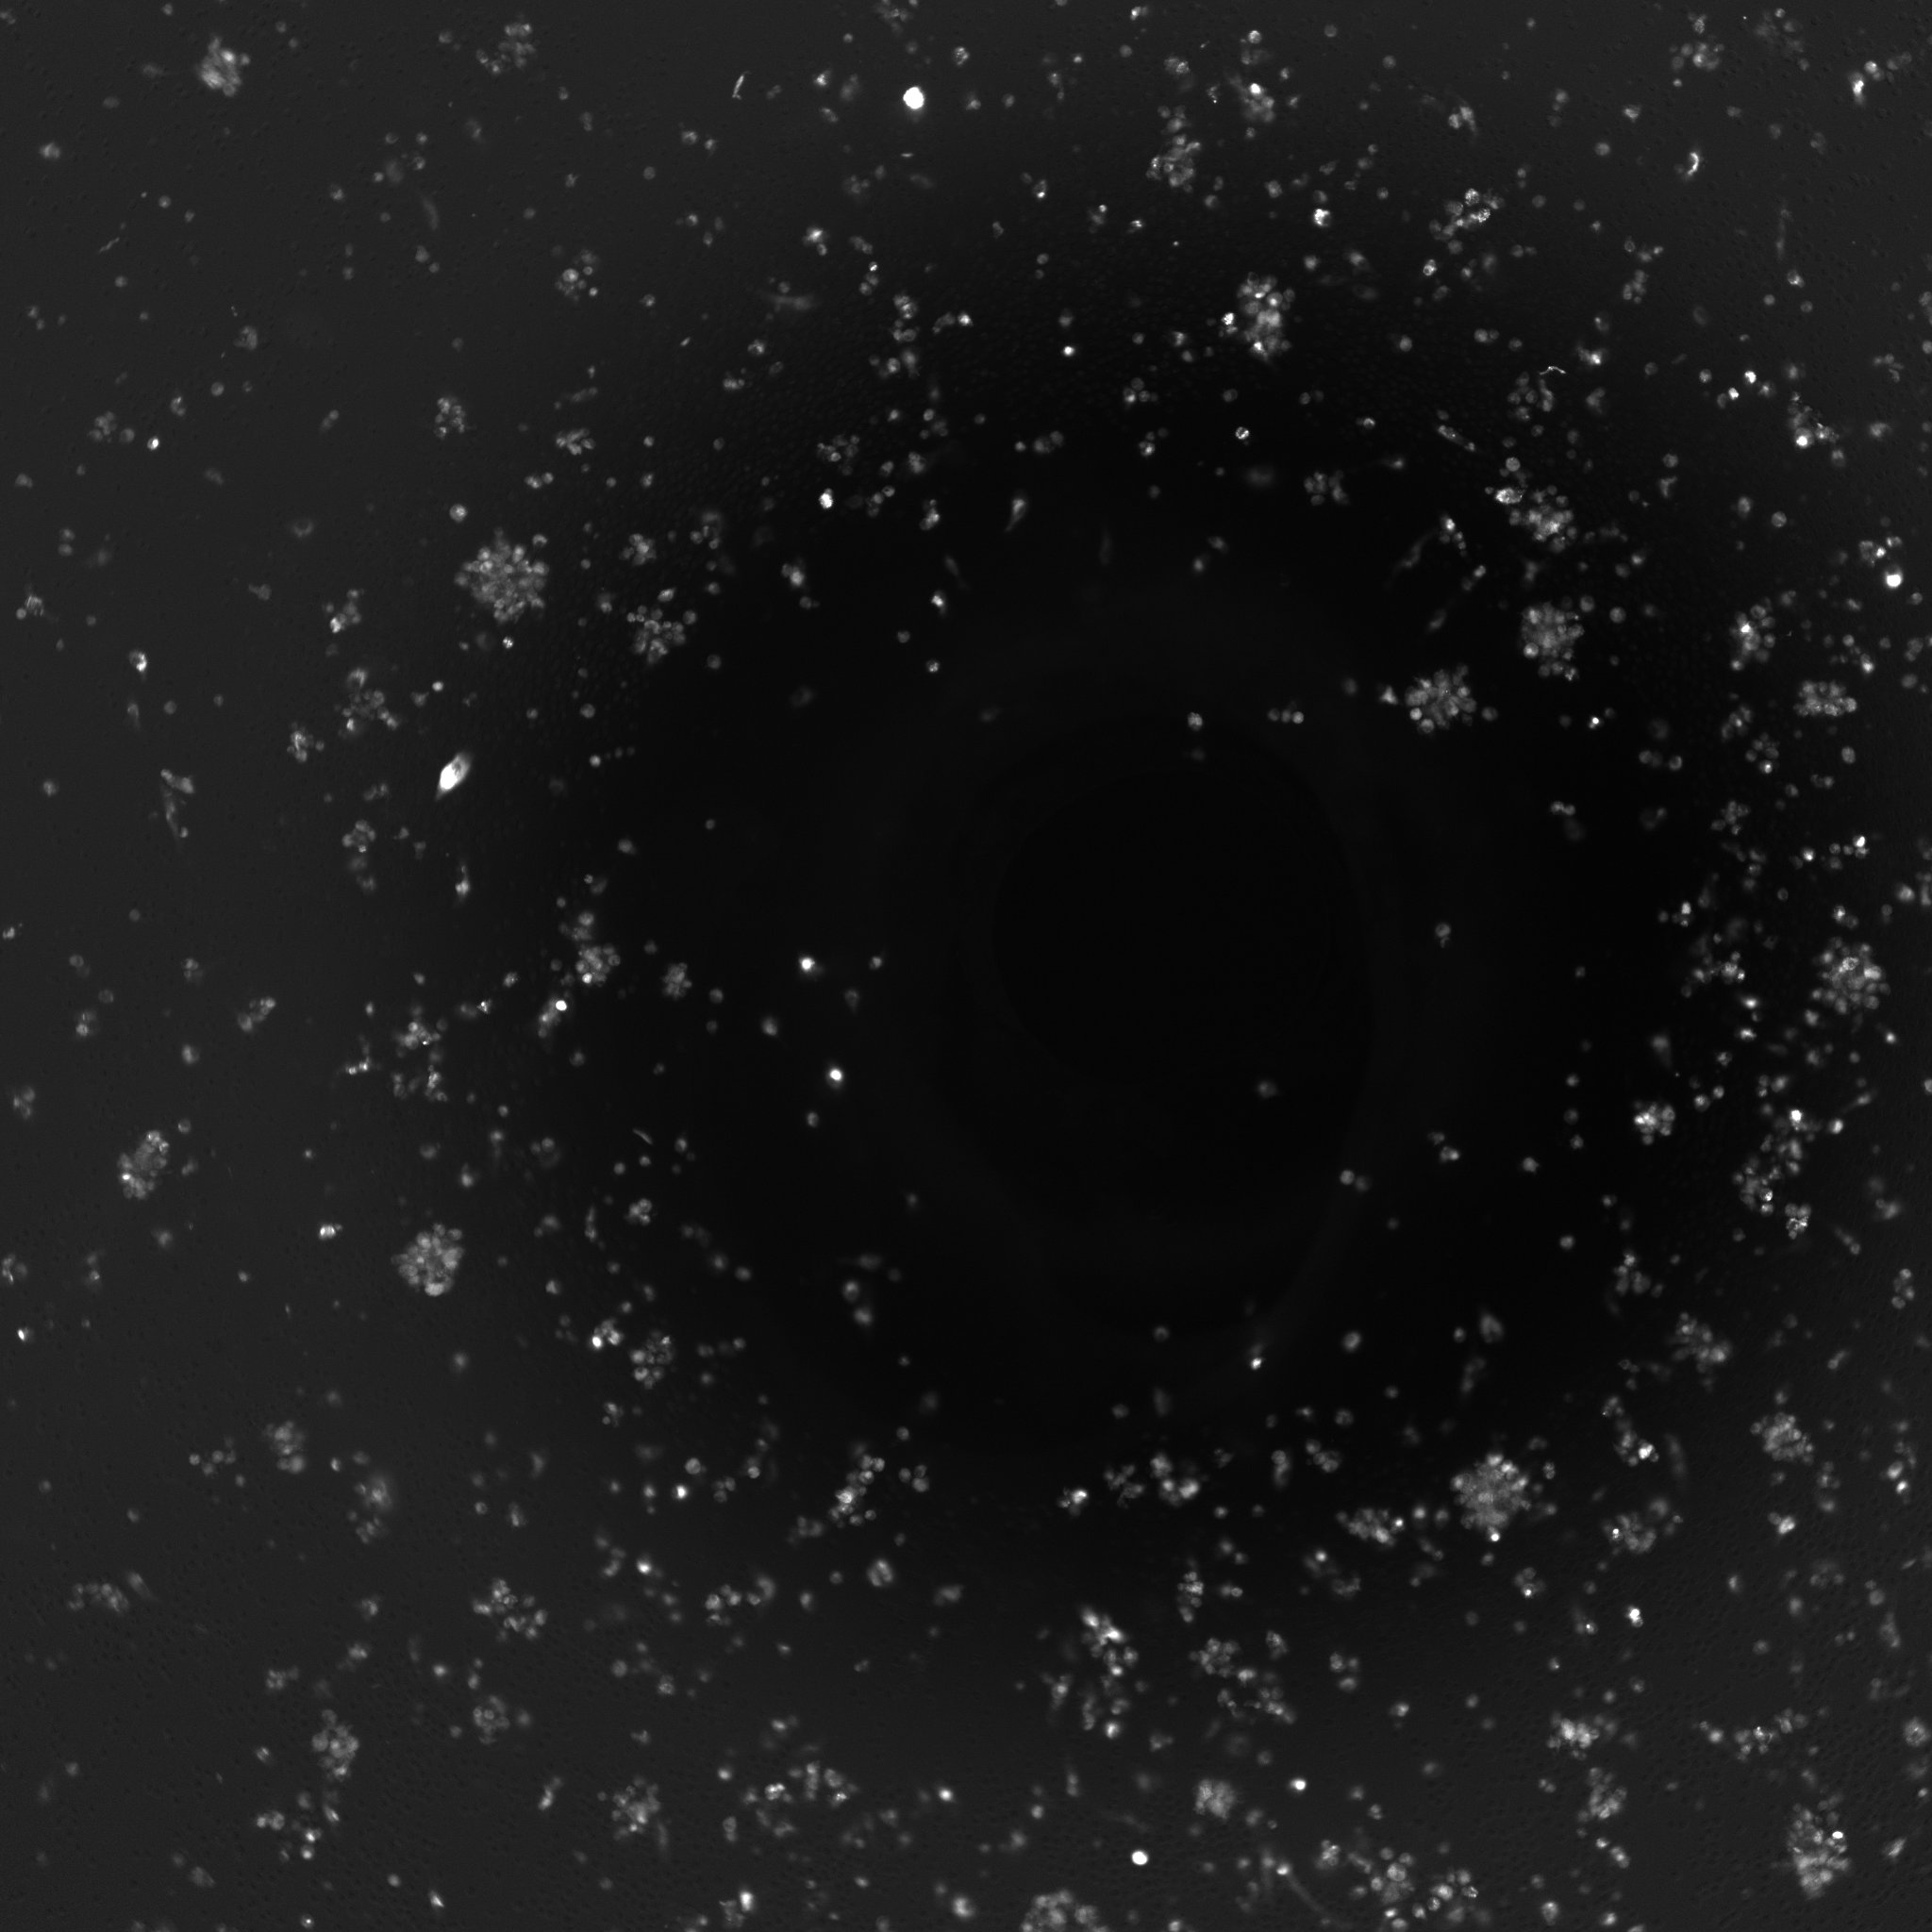
\includegraphics[width=\textwidth]{dissertation/figures/faulty_dcell.jpg}
        \caption{Red dye (DCs) view}
        \label{subfig:dc}
    \end{subfigure}
    \caption{Different views of an image which contains ``Faulty" patches. The fault is likely coming from a drop of water in the well. \protect\subref{subfig:tcell}, \protect\subref{subfig:dc} have been brightness-adjusted for visualisation.}
    \label{fig:noisyimage}
\end{figure}

\bigskip
\subsubsection{Labelling}

\hfill\\
\hfill\\
Each plate came with an Excel sheet giving information about plate layout. Each well was assigned a letter and a name, and the Excel sheet contained information about the stimulation, drug compound ID number, and compound concentration used for each well. These Excel sheets were not automatically parsable, since types of drugs or location in the sheet might vary from one to the next, hence labelling had to be hardcoded and handchecked. 

\subsection{Combining images to qualify interaction} \label{subsec:combining}

To summarise the section above, we made sure that for each well representing an experimental condition, we obtained two images of interest: an image of T cells, and its counterpart image of dendritic cells. While these were obtained separately with the help of fluorescent dyes, they were still captured from the same well in which they were placed together. Hence, for us to gain any understanding of cell interaction from these images, we needed to combine them one way or another. 

We decided to combine each black-and-white T cell and DC image in one RGB image. Computationally speaking, an RGB image is represented by a multi-dimensional array of three arrays. Each of these arrays corresponds to a colour channel: red, green, or blue. The dendritic cell images were obtained through fluorescent red dye screening, so the red channel of the image was set to this image. Similarly, the T cell images were obtained through fluorescent green dye screening, so the green channel of the image was set to this image. The blue channel of the RGB image was left blank. The resulting RGB image thus allowed us to visualise T cells in green, DCs in red, with close overlap between those cells will in orange hues. Figure \ref{fig:combined} illustrates a sample of combined sub-images after this operation was completed.

This combination allowed us to visualise areas of proximity in cells as well as areas of overlap. As such, this visualisation provides us a means of qualifying interaction between the different types of immune cells. 

\begin{figure}[h]
    \centering
    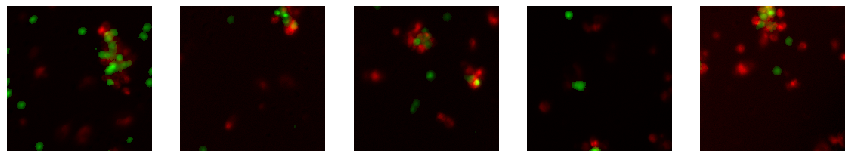
\includegraphics[width=\textwidth]{dissertation/figures/combined_cells.png}
    \caption{Random sample of five RGB images, where the red channel contains the dendritic cells and the green channel contains the T cells.}
    \label{fig:combined}
\end{figure}

\section{Image segmentation} \label{sec:segmentation}

Image segmentation refers to the process of separating out the parts of interest of an image into different `segments' or objects. In our context, applying image segmentation to our dataset had two purposes. The first was to use image segmentation as a method to separate the background from the cell objects for background correction. The second was to use it to obtain binary objects of the cells in order to compute numerical data about cells in the images. 

\subsection{Background correction} \label{subsec:correction}

Although we have defined a method to perform some background noise reduction in images in Section \ref{subsec:preproc}, this method might not be able to catch all irregularities in the background. As such, we wanted to be cautious and explore some alternatives. 

All the images in the original, uncombined dataset were black and white, with the details of interest (i.e. the cells) in bright white spots. However, as discussed in Section \ref{subsec:preproc}, the images could contain noise coming from grey details in the image that the naked eye cannot see immediately. Moreover, our noise removal methods might not be foolproof. There might be some noise remaining that could influence how a model learns. The best way for a model to learn about cells only is to only provide pixel values for cells, with a background sent to 0. Hence, we needed a method that will separate out the cell pixels from the background. We achieved this by obtaining a binary mask of the image, such that the white pixels of the binary image corresponded to the cells, and the dark pixels corresponded to the background. We tested two methods for doing this: K-means and thresholding, which will be described further in Section \ref{sec:implementation}.

Once a binary mask is obtained through these methods, we removed the background of the original image by multiplying it with the mask, a procedure known as \textit{masking}. If the binary mask is satisfactory, the output of this image should only contain the cells, which will have kept their detail, while the background will have been blacked out. 

\subsection{Quantifying interaction}

The process used in \autoref{subsec:combining} describes a way of visually qualifying interaction between immune cells from combined images. However, we are also interested in quantifying interaction and obtaining a numeric value for the interaction between the T cells and the dendritic cells.

We can use the same method as described above to obtain the mask of the cell objects in each image before combination. This pair of masks can be used for further calculations. A common metric for evaluating image segmentation quality is \textbf{intersection-over-union (IoU)}, also known as the Jaccard index \citep{rahman_optimizing_2016, rezatofighi_generalized_2019, beers_deep_2019}. This metric is normally used to evaluate how successful the segmentation of an object in an image is by comparing the segmented object to its ground truth value. It is computed from binary objects as shown in \autoref{equation:iou}. The process of calculating overlap in our dataset is illustrated in \autoref{fig:mask_overlap}.

\begin{equation}
    IoU(X,Y) = \frac{X \& Y}{X | Y}
    \label{equation:iou}
\end{equation}

In this case, we can use the IoU as a metric for area of overlap between two separate cell objects: the T cell objects and the dendritic cell objects obtained from the same sub-image. We can use the concept of overlap to quantify the level of interaction between cells. These overlap numbers will be used as label input to a deep regression model. Each pair of images which will be combined will be associated with an overlap value. The aim will be to evaluate whether we can train a model to predict a numeric value of interaction from an image.

\begin{figure}[h!]
    \centering
    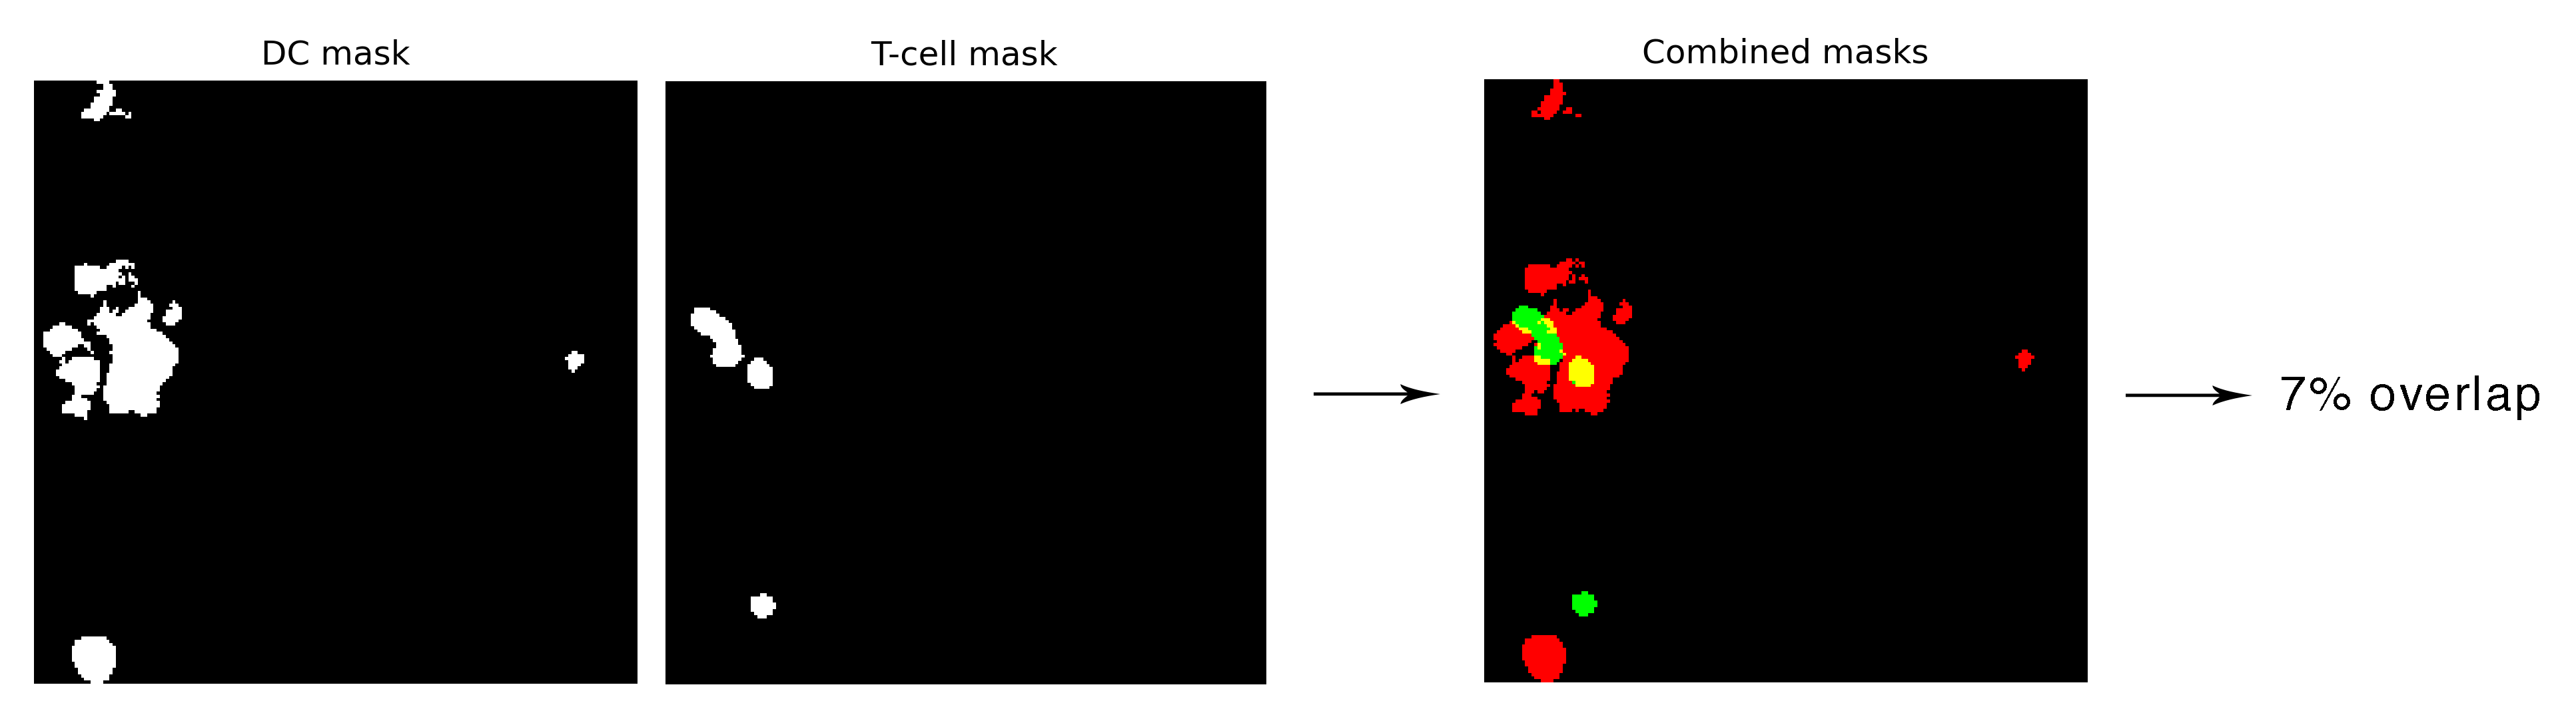
\includegraphics[width=0.8\textwidth]{dissertation/figures/mask_overlap_operation.png}
    \caption{Example calculation of the numerical overlap between two sets of immune cells. The overlap is visually represented in yellow. In this example we obtain a 7\% overlap with intersection-over-union of the two masks.}
    \label{fig:mask_overlap}
\end{figure}

\section{Deep learning models}

The following two sections highlight what kind of deep learning models we used and their specific purposes of in the context of our research. Their general structure is highlighted in Figure \ref{fig:connected_models}.

\begin{figure}[h]
    \centering
    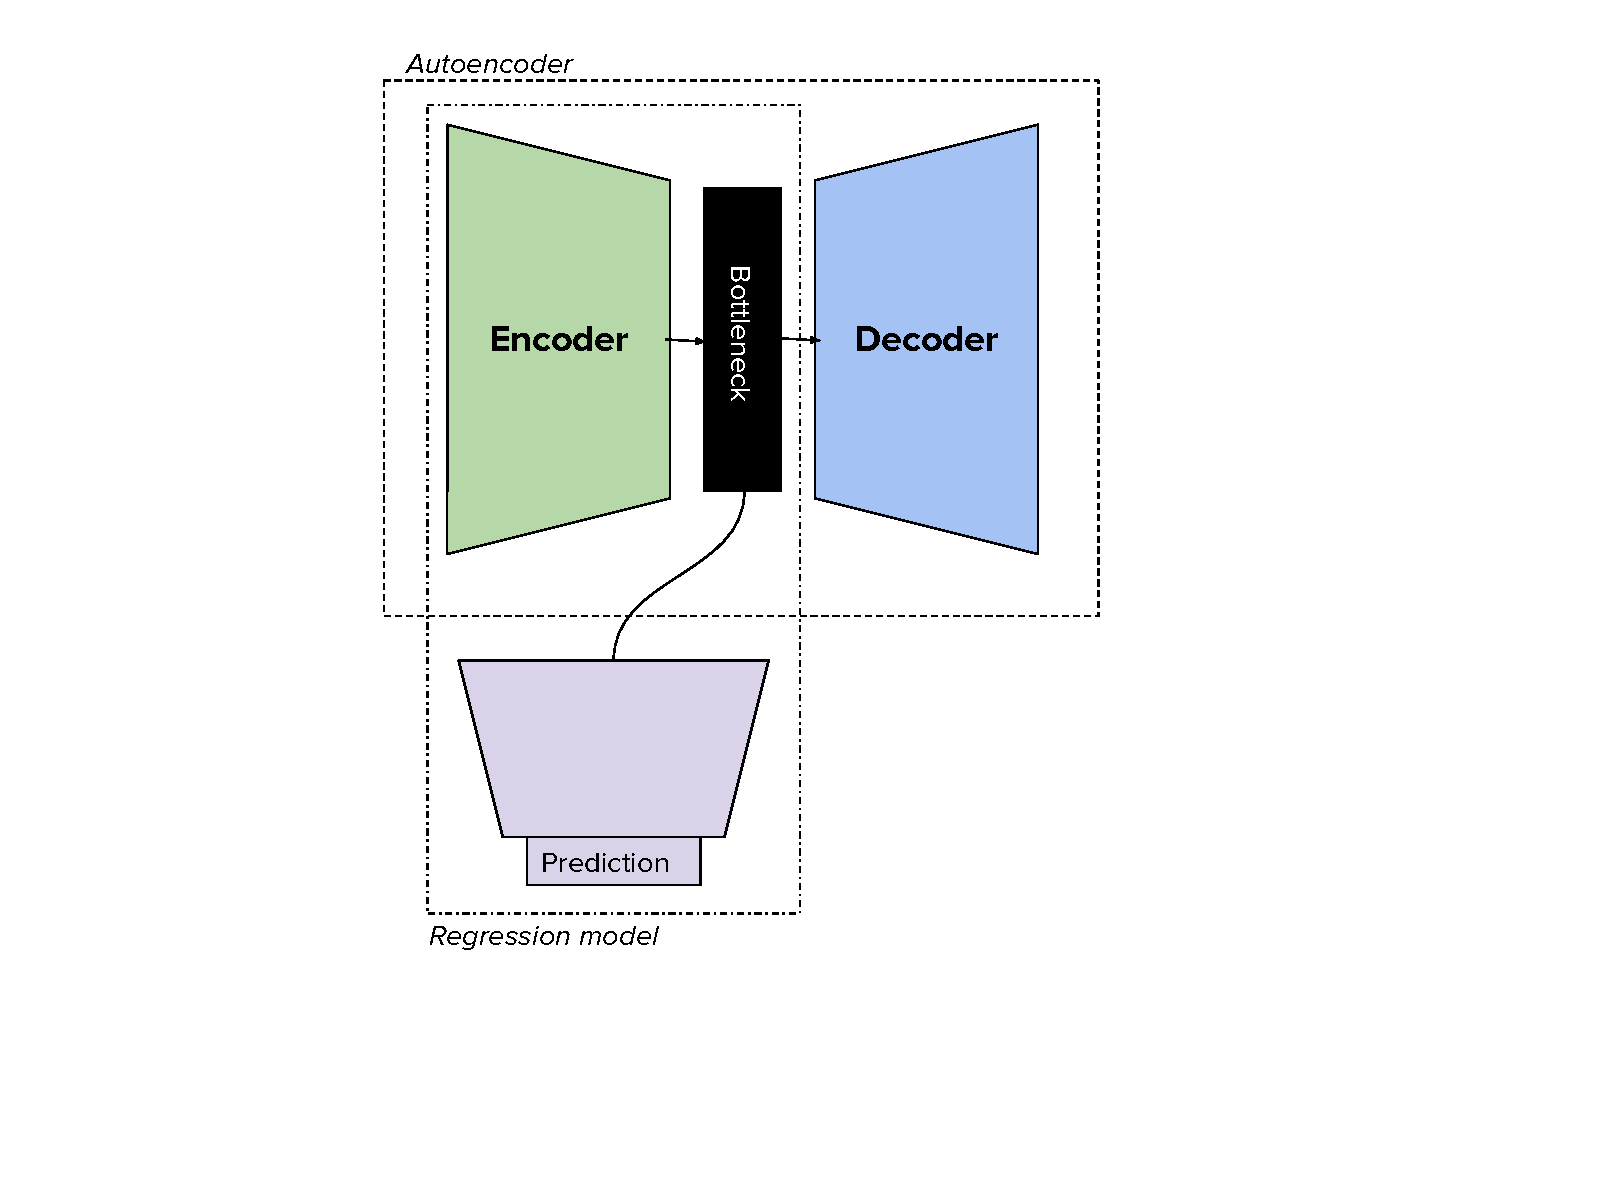
\includegraphics[width=.5\textwidth]{dissertation/figures/autoencoder_regression_connection.pdf}
    \caption{Schematic diagram of the models to be implemented. The encoder layers will transform the input into a smaller coded representation, from which the decoder layers will create a reconstructed version of the image. The encoder layers will then be connected to a regression model, from which we hope to make predictions on how much interaction is perceived in an image. The bottleneck representation will also be fed into the UMAP algorithm.}
    \label{fig:connected_models}
\end{figure}

\subsection{Autoencoder for visualising high dimensional data}

As described in Section \ref{sec:deepl_bg}, autoencoders are a particular type of neural network built with symmetrical layers around a bottleneck. The aim of an autoencoder is to map an input to itself as close as possible, while reducing its dimensions.

Different types of autoencoders exist. As our input consists of images, we set ourselves to implement a convolutional autoencoder. The hope was that if an image is reduced to a certain number of dimensions through convolutional neural networks, and another convolutional neural network is able to reconstruct the original image very closely just based on that compressed representation, then that smaller code representing an image is a good enough representation of the original input that can be fed into other models or algorithms. 

The first aim for our autoencoder was to reduce the dimensions of our image input, as the size of the data points made it slow for data visualisation techniques to process. Furthermore, we hoped that the most important and distinguishing features of an image would come through the neural network layers and be collated in the bottleneck layer of the model. 

High dimensionality visualisation techniques such as t-sne and UMAP can help visualise if there is an inherent structure to the data. We wanted to use this as a tool for analysis of immune cells interaction. We decided to use UMAP as our visualisation tool as both techniques yield similar structures as shown in \autoref{sec:bg_visualisation}, but UMAP has been shown to outperform t-SNE time-wise. This also allowed us to experiment with UMAP's different parameters more easily, and to observe different structures of clusters in the data.

We wanted to be able to qualify interaction only from an image, without our model being supervised with labels about the image's associated experimental condition. This could be evaluated from a UMAP projection and whether or not clusters were formed around the same experimental conditions. If such successful groupings were found, it would allow us to show that different experimental conditions yield structurally similar cell interactions. 

\subsection{Regression model for quantifying interaction in unseen images}

We also developed a deep regression model. Our regression task was to predict overlap values on unseen images. We used our autoencoder as a building block for a deep regression model. Again, we hoped that the autoencoder would successfully extract the most important features from the images through convolution operations and this would be a good starting block.

We used the encoder block of the model and extended it in a regression structure with fully connected layers. This regression model took images and associated overlap values as input for training. We could then assess whether or not the model successfully predicted interaction values from an image of T cells and dendritic cells. We would also be able to evaluate whether this was a faster approach than segmenting cells and calculating their overlap. Similar regression models could also be trained with other interaction metrics easily.
\chapter{Implementation} \label{sec:implementation}

All development of the methods detailed in this section was done using Python.

\section{System diagram}

Figure \ref{fig:system} can help the reader to gain understanding how each of the materials and methods used as described in Section \ref{sec:mm} fit together.

\begin{figure}[h!]
    \centering
    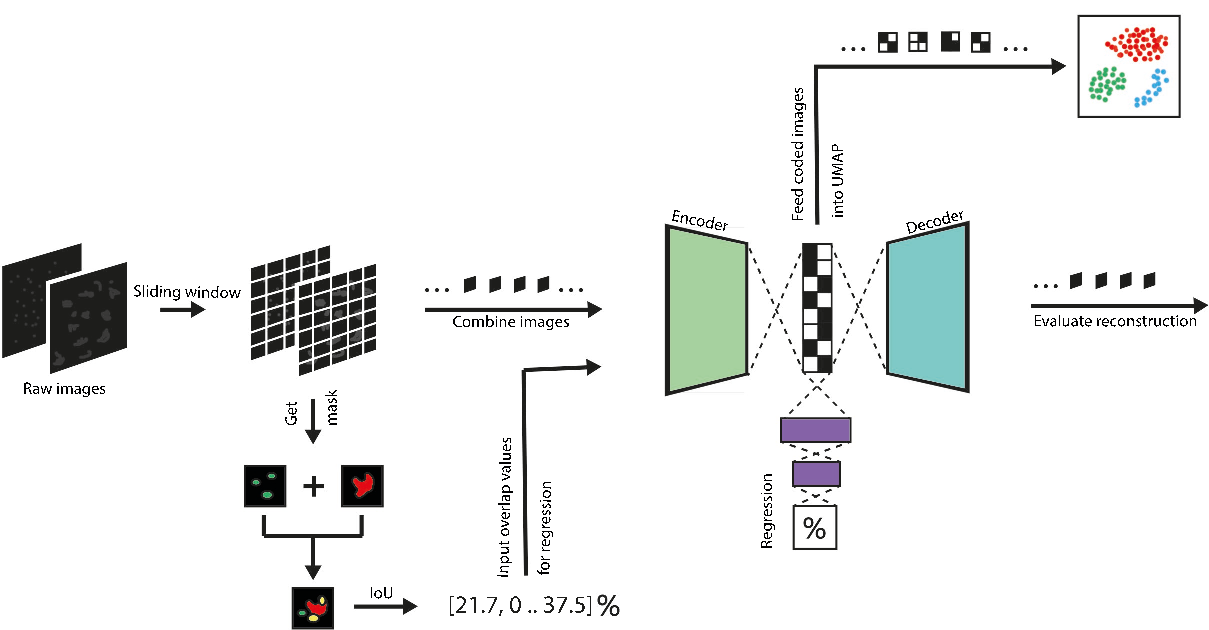
\includegraphics[width=\textwidth]{dissertation/figures/system_diagram.pdf}
    \caption{[TO ANNOTATE] System diagram showing how each image will be decomposed and analysed. The images will be transformed into smaller patches, from which we can gain overlap labels. On one hand, the smaller images will be fed into an autoencoder to accomplish dimensionality reduction and evaluate the success of projection of this smaller data in a two-dimensional plane. On the other hand, the smaller images will be fed in a regression model with the overlap labels in order to train a deep neural network for a regression task.}
    \label{fig:system}
\end{figure}

\section{Pre-processing}

Pre-processing steps are best illustrated through a diagram as shown in Figure \ref{fig:preprocessing}.

\begin{figure}[h]
    \centering
    \missingfigure[]{Figure showing pre-processing steps: raw images -> gridded images: 1. remove noise and normalise 2. obtain overlaps 3. combine images}
    \caption{Caption}
    \label{fig:preprocessing}
\end{figure}

Images were processed with a sliding window of size 192x192 as we wanted a window that was large enough to contain a few cells but also wanted to make it smaller to be able to reduce individual image dimensions further. A sliding window of 192x192 yielded 100 patches as our images were originally of size 2048x2048.

[further explanations?]

\section{Image segmentation}

Performing cell segmentation from grayscale microscope images of cells has been researched and is necessary when the cells to be studied in an image have not been separately labelled in one way or another. In our case, cell segmentation does not need to be applied as the images of T-cells and dendritic cells have been captured separately through fluorescent dyes. Instead, we are interested in using segmentation techniques to obtain the mask of each type of immune cell for the purposes of background correction and interaction quantisation, as explained in Section \ref{sec:segmentation}.

As our dataset pre-separated the type of immune cells and the cells were bright blobs on a background, we hoped that obtaining masks from each image would be straightforward. This section describes the methods we explored for this task. Both k-means and thresholding methods yielded good results and their specifics are detailed below.

\subsection{\textit{k}-means colour clustering}

k-means has been shown to perform well on image segmentation by quantising the number of colours in an image into \textit{k} clusters. Formally, k-means aims to partition data points in an array into \textit{k} sets such that the variance between points within clusters is minimised. In our case we wanted to use k-means to transform our black-and-white images of immune cells into bichrome images that we could use as masks. [The following pseudocode details the process of K-means.]

\begin{algorithm}[h]
    \DontPrintSemicolon
    \KwData{$I$, an array of pixel values making an image.\;
    $k$, the number of colours to partition the image's colour palette to.\;}
    \KwResult{A set of $k$ clusters.}
    \Begin{
        Initialise $k$ objects picked from $I$\;
        \While{clusters are still changing}
        {
           Assign each item $i$ in $I$ to the cluster with closest mean value\;
           Recompute the mean of each cluster\;
        }
    }

\caption{Pseudocode for the k-means algorithm applied to image segmentation.}
\label{alg:kmeans}
\end{algorithm}

k-means clustering is conveniently offered by multiple libraries in Python. We looked at both scikit-learn's and OpenCV's k-means. scikit-learn is a general library  for machine learning tools, while OpenCV is a more specialised library built for Computer Vision purposes. Both their k-means functions are straightforward to initialise and use. Their performance was benchmarked in order to select the best one. The table below reports times for k-means with \textit{k}=2, 10 iterations, and each of the random and optimised methods of initialising centroids.

\begin{table}[h]
\centering
\begin{tabular}{|l|l|l|}
\hline
\textbf{Initialisation} & \textbf{OpenCV} & \textbf{Scikit-learn} \\ \hline
Random                                   & \multicolumn{1}{r|}{18.9s}       & \multicolumn{1}{r|}{165s}              \\ \hline
k-means++                                & \multicolumn{1}{r|}{29.3s}       & \multicolumn{1}{r|}{139s}              \\ \hline
\end{tabular}

\caption{CPU times for OpenCV's and scikit-learn's k-means tool ran on 1,000 samples of 192x192 pixels with different methods of initialising centroids.  The computation was ran on a 2015 MacBook Pro with 2.7 GHz i5 core and 8 GB memory.}
\end{table}

As we can see OpenCV outperforms scikit-learn in all cases. OpenCV for Python is a wrapper library around the original OpenCV code built in C++, which gives it a boost in performance. OpenCV's k-means was thus selected. Initially, k-means centers were initialised randomly in development for the boost of performance. However, during validation it was found that this method of initialisation was yielding highly different results for the intersection-over-union metric at every run. Hence, some speed was traded for consistency and the kmeans++ center initialisation method was picked instead.

\subsection{Thresholding}

An alternative to k-means in the case of black-and-white images is thresholding. We decided to explore this option as it could have performance improvements compared to K-means.

Thresholding refers to the process of converting a grayscale image to a binary image of pixels. Pixels above a set threshold are set to 1, and the rest of the pixels below that threshold are set to 0. Thresholding depends on pixel distribution analysis. Usually, thresholding works well for images which have different peaks of pixel values in their distribution. We can then pick the value which seems to separate out the two peaks as our threshold. However, in the case of our images we had one visible peak of pixel values and could not identify a viable threshold from the histogram. Figure \ref{fig:thresholdhist} illustrates this.

\begin{figure}[h]
    \centering
    \begin{subfigure}{0.45\textwidth}
        \centering
        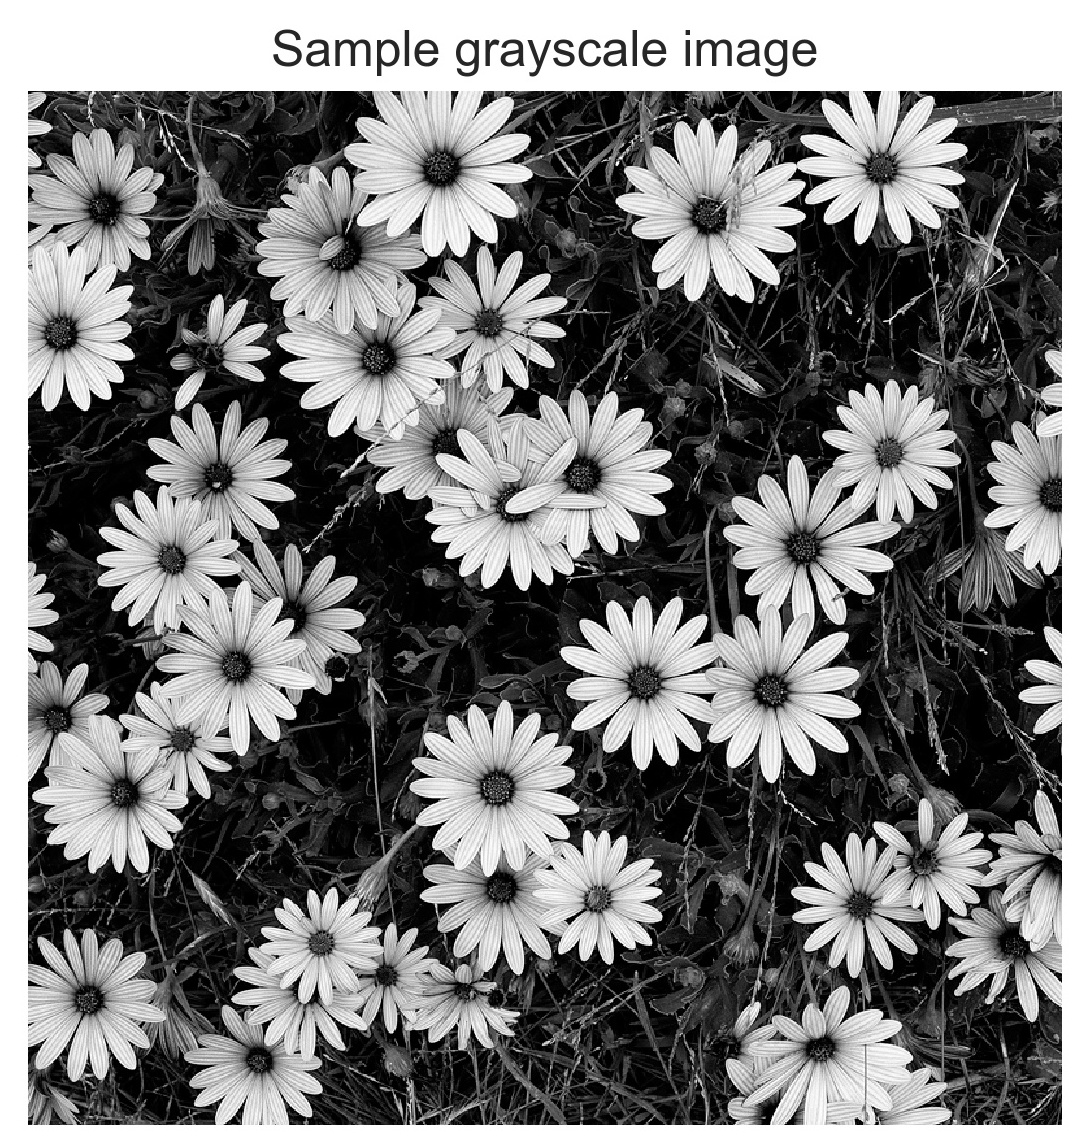
\includegraphics[width=.5\textwidth]{dissertation/figures/sample_grayscale.jpg}
    \end{subfigure}
    \begin{subfigure}{0.45\textwidth}
        \centering
        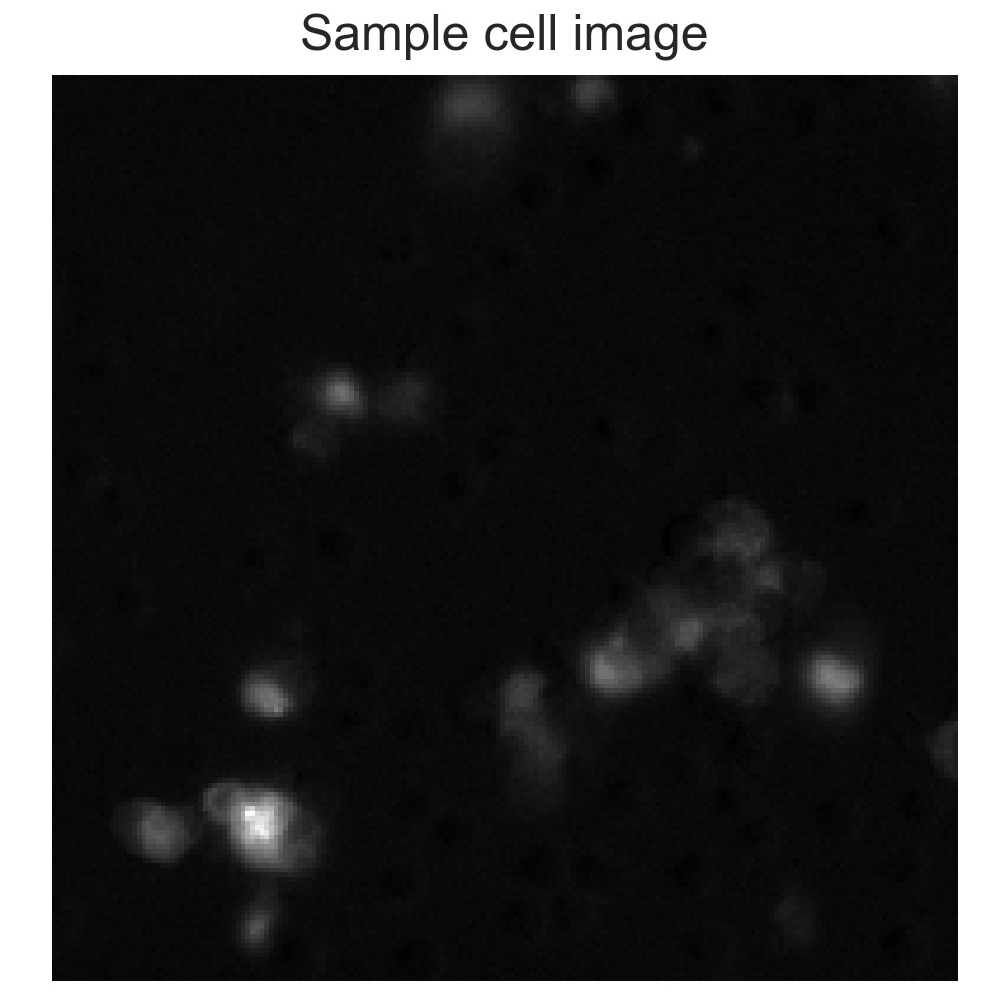
\includegraphics[width=.5\textwidth]{dissertation/figures/sample_cell.jpg}
    \end{subfigure}
    \begin{subfigure}{0.45\textwidth}
        \centering
        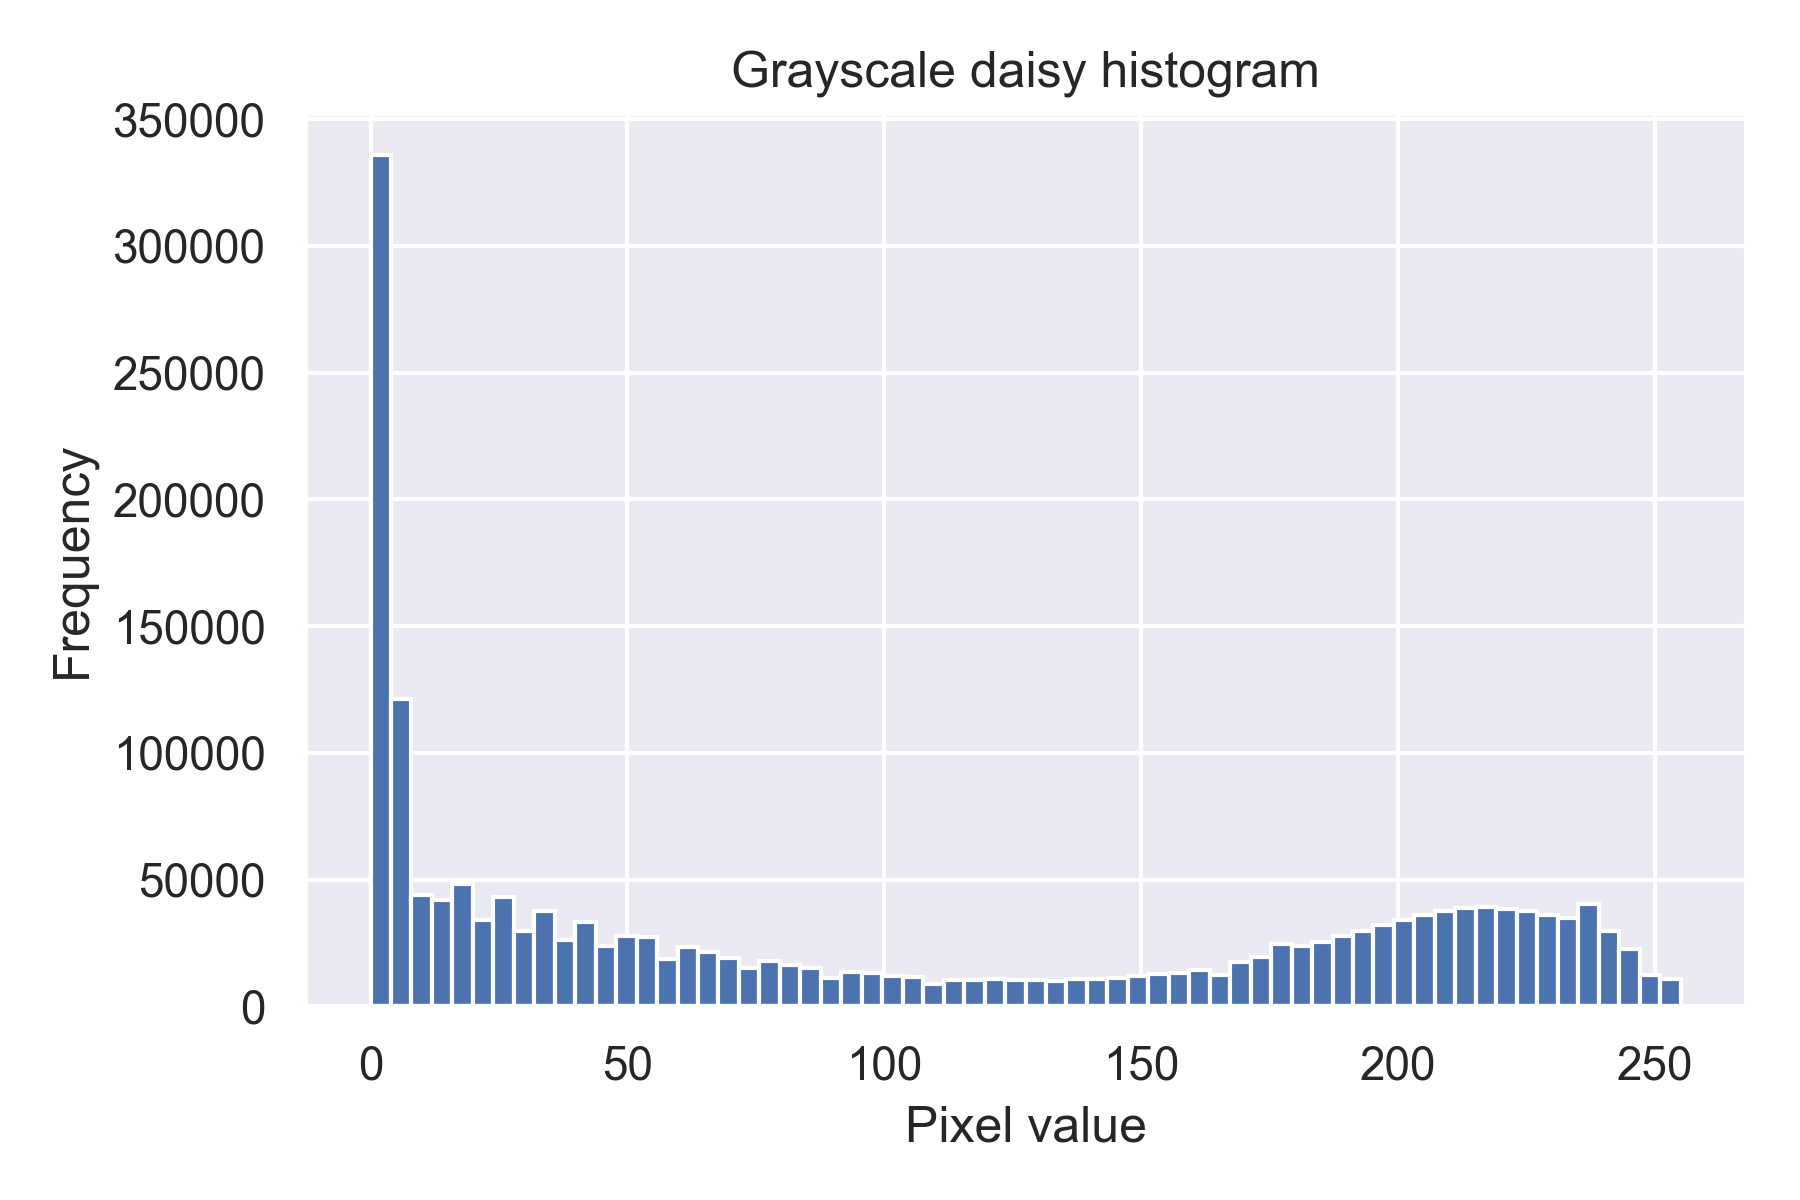
\includegraphics[width=.5\textwidth]{dissertation/figures/grayscale_histogram.png}
    \end{subfigure}
    \begin{subfigure}{0.5\textwidth}
        \centering
        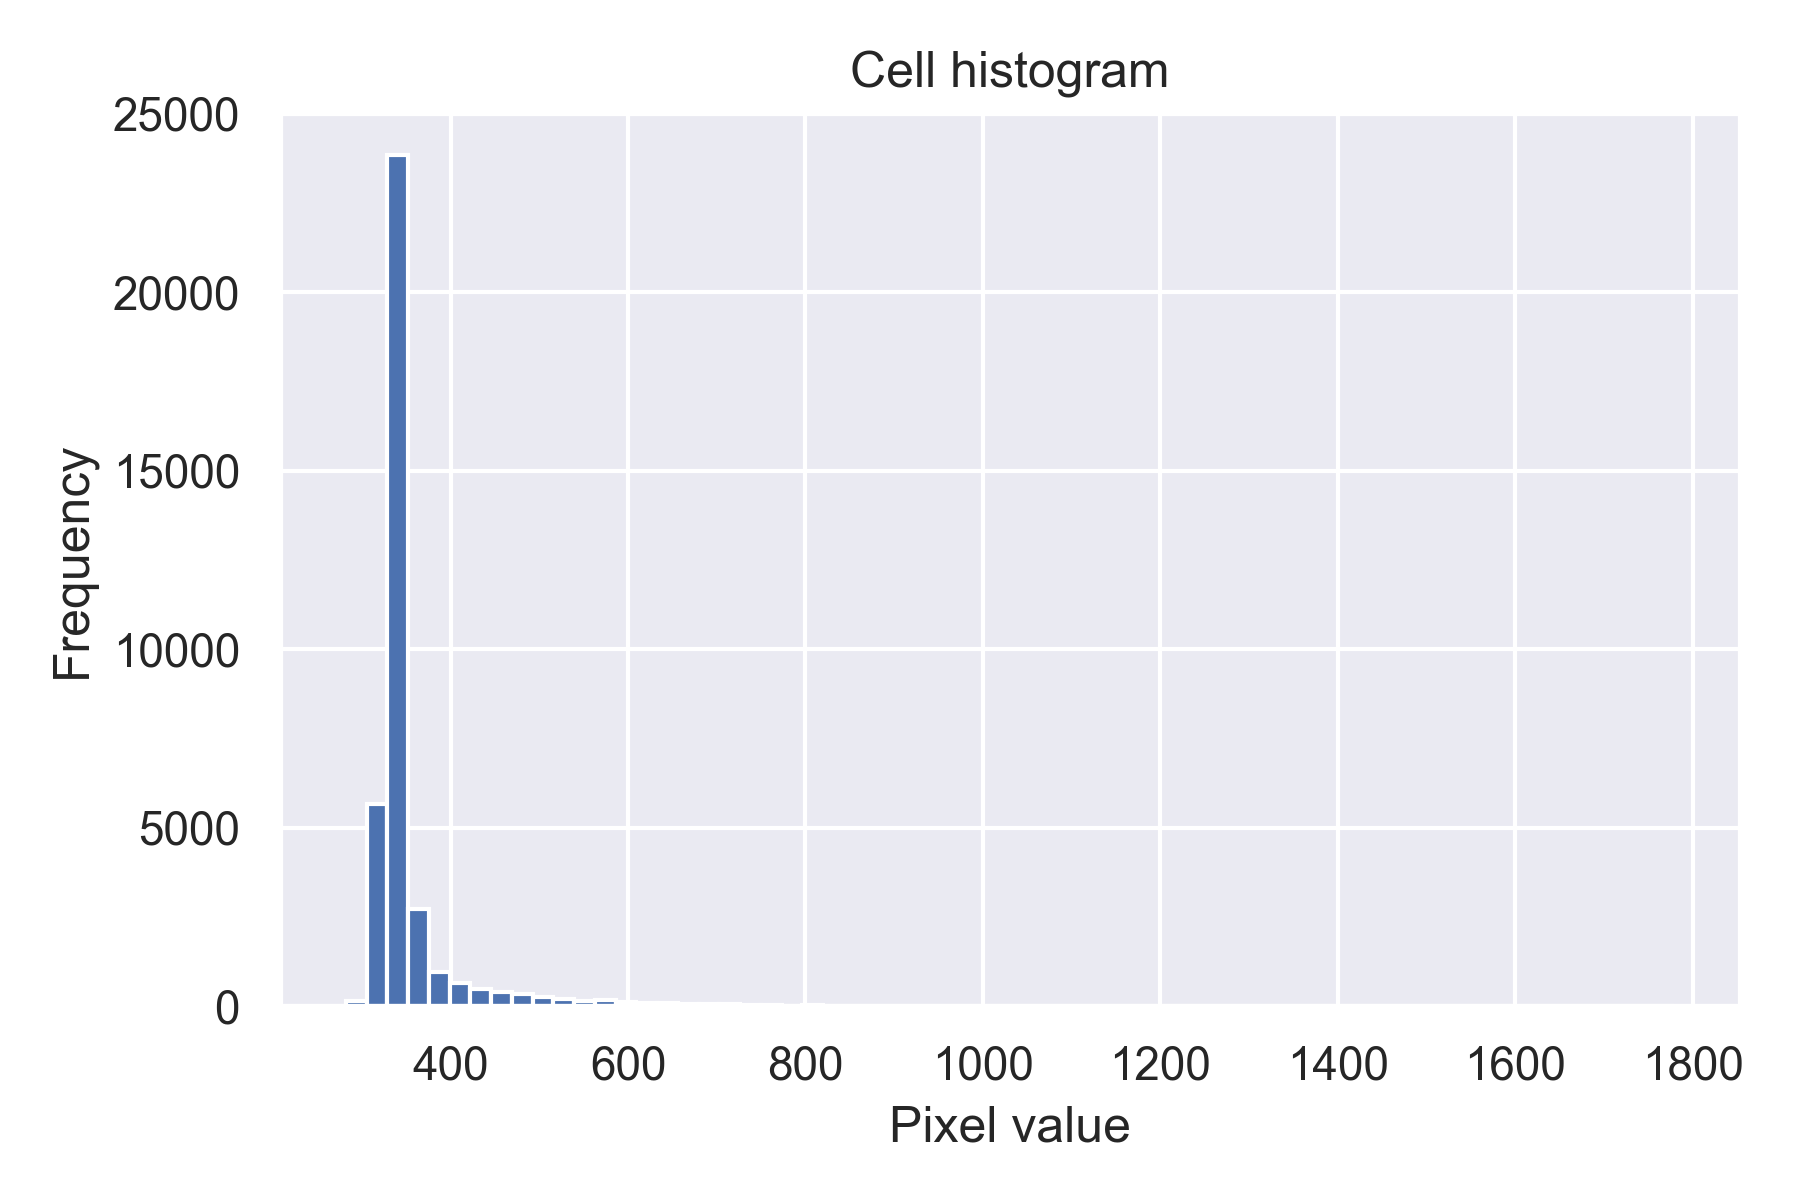
\includegraphics[width=.45\textwidth]{dissertation/figures/cell_histogram.png}
    \end{subfigure}
    \caption{Example images and their histogram. As we can see the grayscale image of lillies has two peaks of frequency, and we can see there is a separation between the peaks at a pixel value of around 110. The grayscale image of a cell has one peak, and there is a smaller frequency of pixel values past that peak, but we cannot identify a specific pixel value as a threshold from the histogram.}
    \label{fig:thresholdhist}
\end{figure}
As such, we had to find an alternative for finding a suitable threshold. First, we selected the mean pixel value as the threshold. This yielded acceptable results, however some noisy pixels still came through the mask (see Figure \ref{fig:thresholdmean}). To fix that problem, the threshold value was set as the sum of the mean pixel value and the standard deviation. This decision was based on the hypothesis that the noise level of an image with a flat structure can be estimated from its variation. Results were satisfactory, as shown in Figure \ref{fig:thresholdstd}.

\begin{figure}[h]
    \centering
    \begin{subfigure}[h!]{0.4\textwidth}
        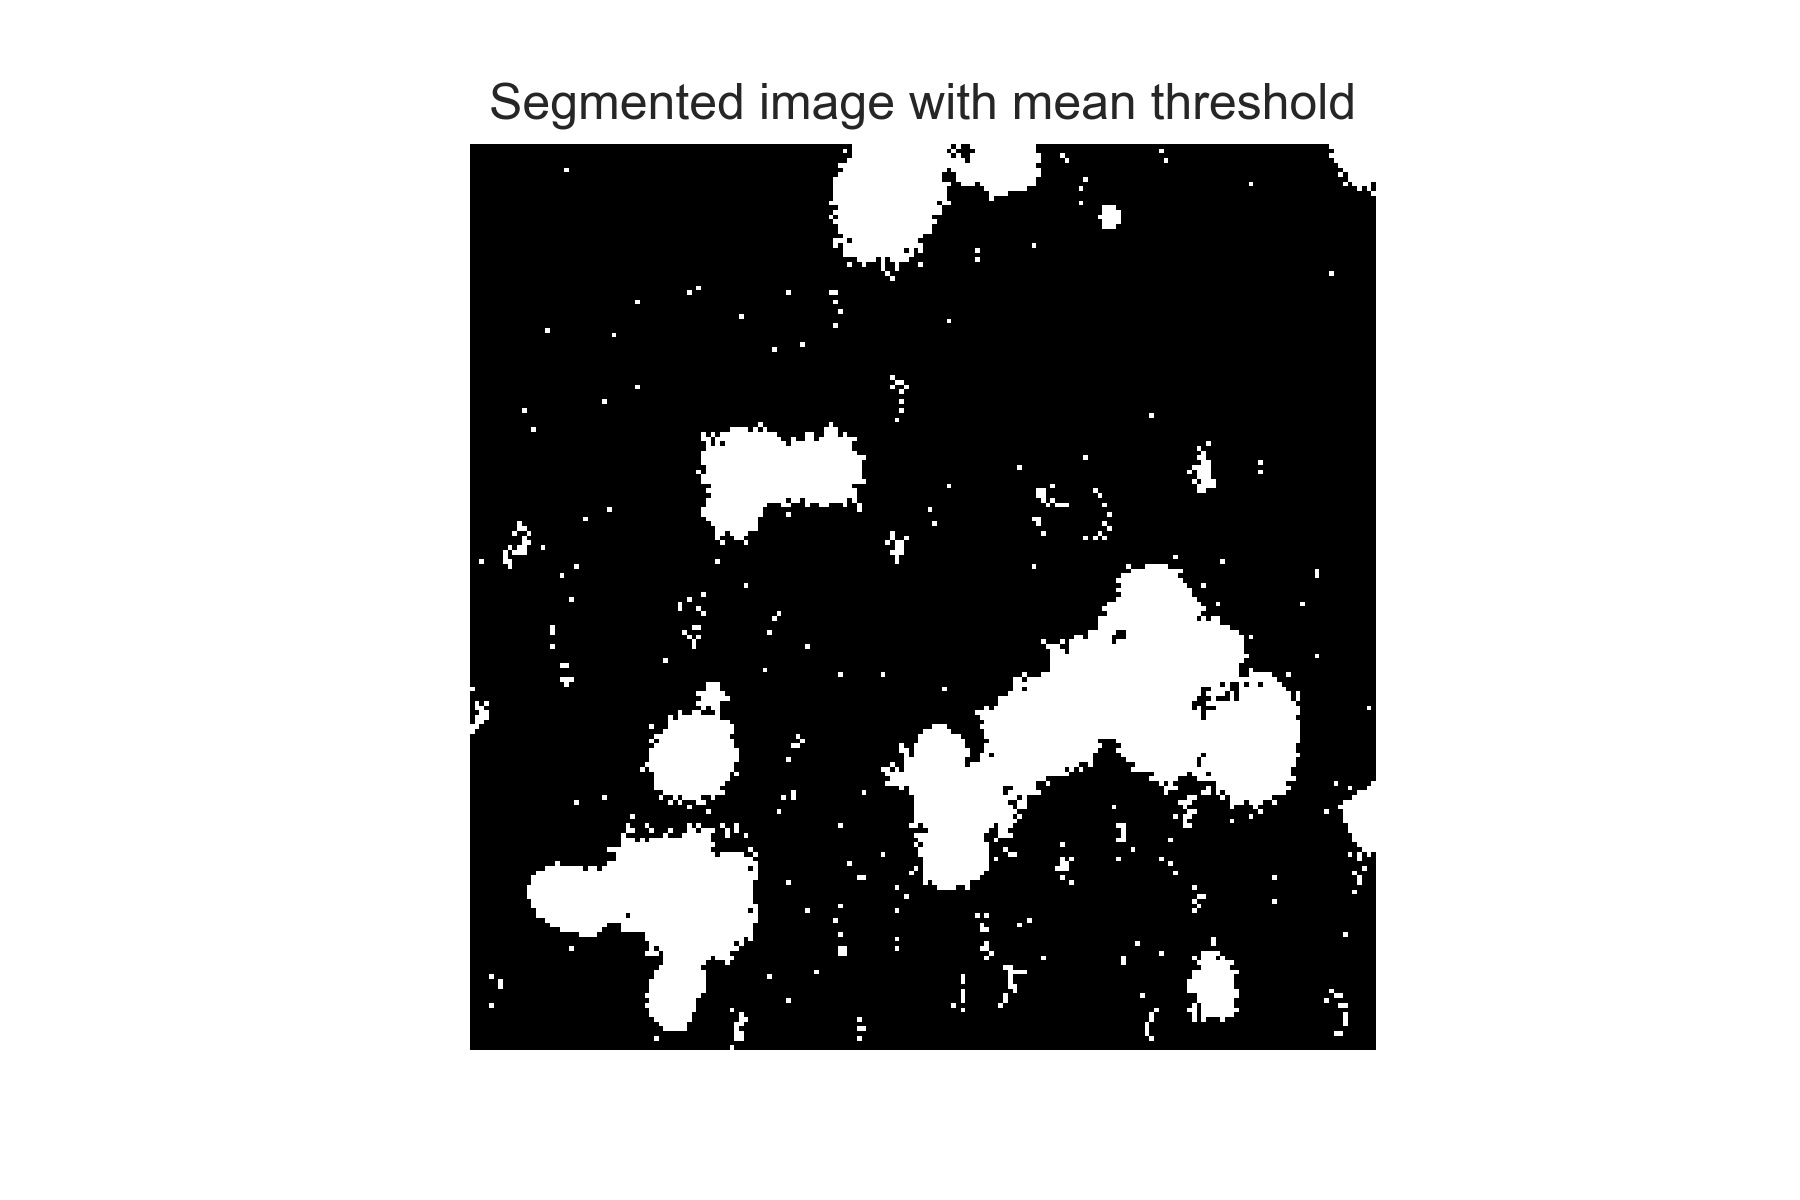
\includegraphics[width=\textwidth]{dissertation/figures/mean_threshold_cell.jpg}
        \caption{Threshold: mean pixel value}
        \label{fig:thresholdmean}
    \end{subfigure}
    \begin{subfigure}[h!]{0.4\textwidth}
        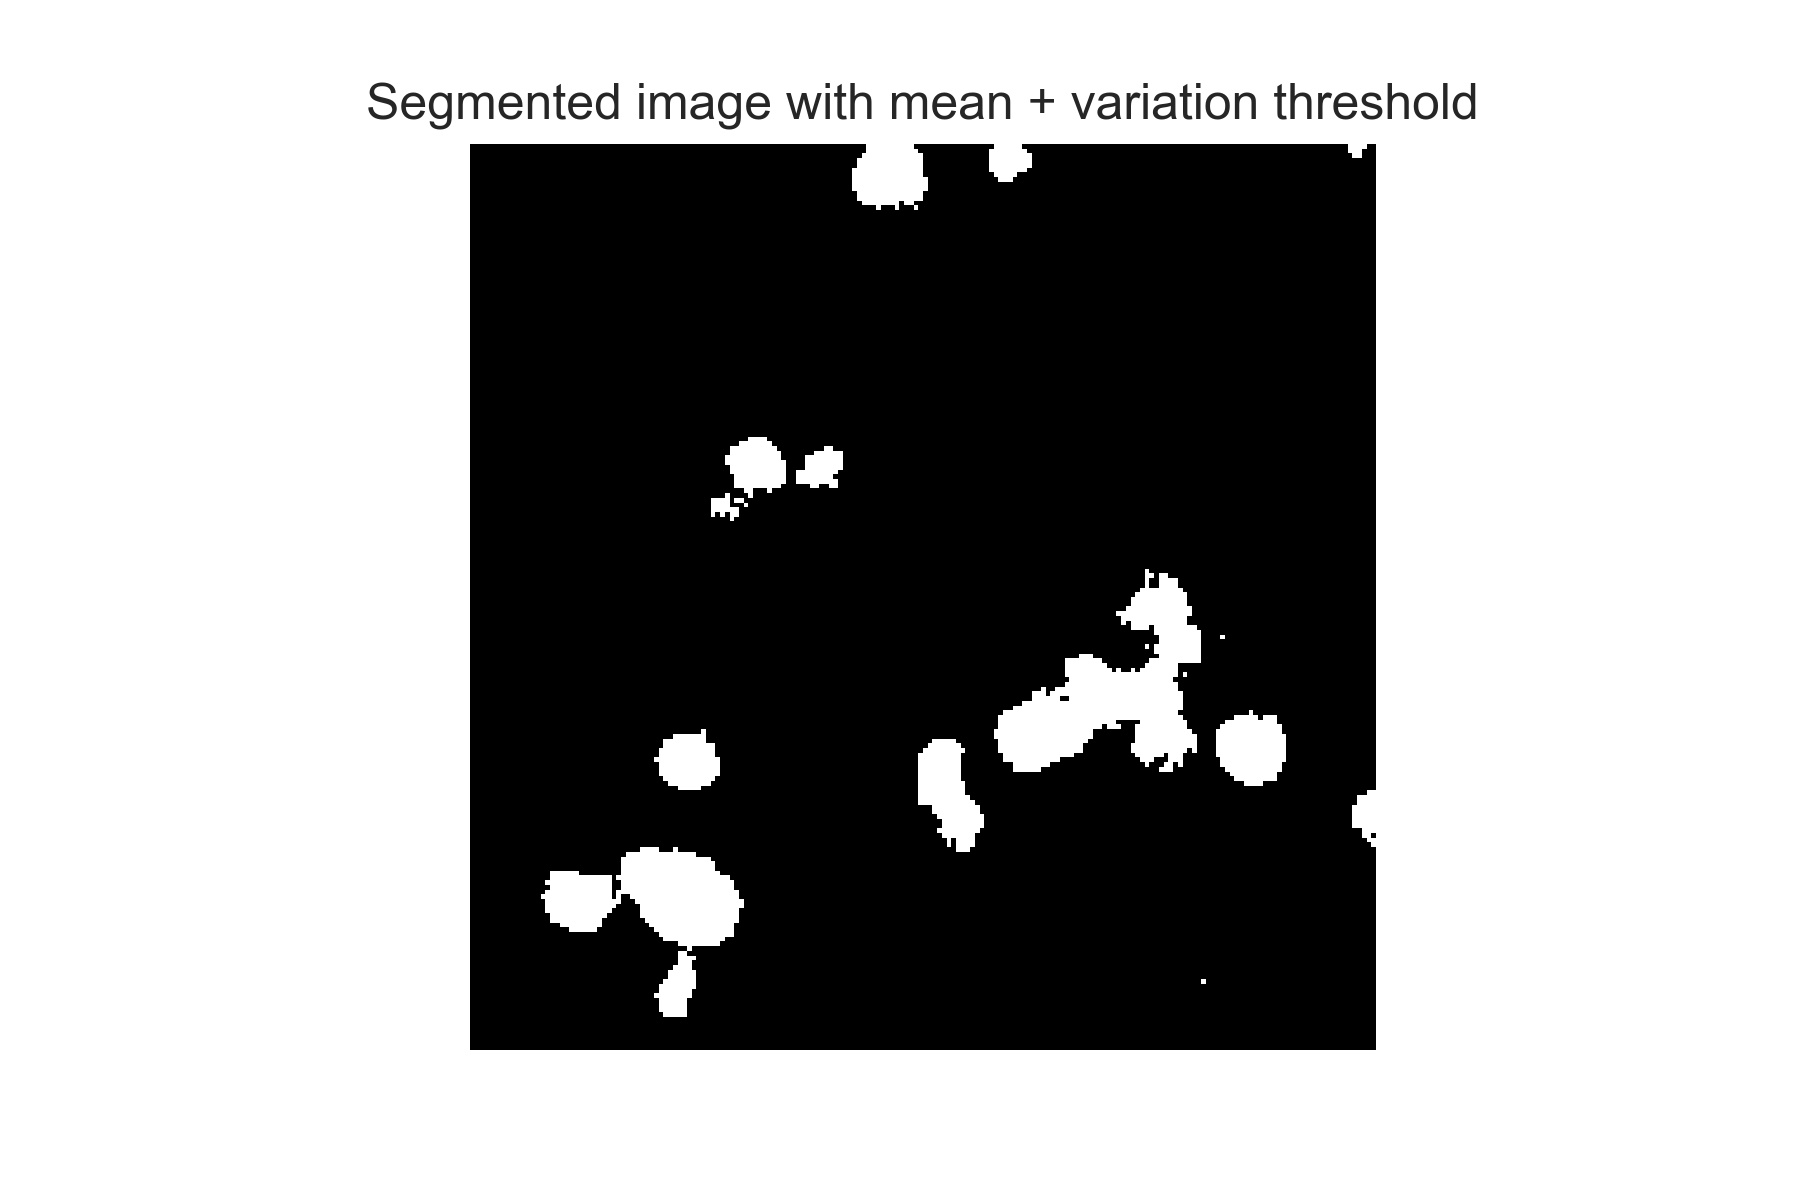
\includegraphics[width=\textwidth]{dissertation/figures/mean_std_threshold_cell.jpg}
        \caption{Threshold: mean + standard deviation}
        \label{fig:thresholdstd}
    \end{subfigure}
    \caption{Segmented images according to different threshold values.}
\end{figure}

Image segmentation through thresholding is also much faster than k-means, with 1,000 images being processed in [360 milliseconds] with the use of NumPy arrays. Nonetheless, masks yielded by k-means are more granular. Figure \ref{fig:maskdiff} shows the difference between the masks obtained through different methods.

\begin{figure}[h]
    \centering
    \missingfigure[]{Binary image showing the absolute difference between a mask obtained with k-means and one obtained with thresholding.}
    \caption{Binary image showing the absolute difference between a mask obtained with k-means and one obtained with thresholding.}
    \label{fig:maskdiff}
\end{figure}

\subsection{UNet}

[mention UNet findings here?]

\section{Autoencoder and regression models}

\subsection{Experimental setup}

As this is a research project based on using deep learning models, a large part of the research involved an iterative process of repetitively tweaking the deep learning models, training them, and evaluating them. Immunology experiments produce a lot of imaging data, and we wanted our models to perform well on unseen data. Moreover, not all datasets contained instances of all classes. We wanted our trained model to be able to deal with such datasets too. As such, we selected the full dataset containing instances for all classes for training our model (see Table \ref{table:datasets}). Part of it was set out for validation and testing. The other two selected datasets were used purely for testing. Table \ref{table:splits} reports the number of samples in each dataset.

\begin{table}[h]
\centering
\begin{tabular}{l|r|r|r}
\hline
\rowcolor[HTML]{EFEFEF}
Dataset       & Train  & Validation & Test   \\ \hline
Full & 16,490 & 2,910      & 10,000 \\
Dual   &        &            & 15,900 \\
DMSO          &        &            & 8,000  \\ \hline
\end{tabular}
\caption{Train-test-validation splits for selected datasets. Models are only to be trained on the full, balanced dataset. The validation set represents 15\% of the training set.}
\label{table:splits}
\end{table}

All deep learning development was done using Keras\footnote{https://keras.io} for Python on a Tensorflow backend. Training was carried out on Google Colaboratory notebooks\footnote{https://colab.research.google.com/} to be able to accelerate computations with Google's GPUs.

While training, we used Keras's callbacks feature to monitor the model's validation loss and change training parameters accordingly. The model would reduce its learning rate by a factor of 0.2 if no improvements in the validation loss were seen over 3 epochs, and it would completely stop training if no improvements were witnessed in validation loss over 5 epochs. Training was usually ran with a batch size of 64 over 40 epochs.

\subsection{Convolutional autoencoder}

The main model to be developed was a convolutional autoencoder. The autoencoder was built for two purposes: obtaining a smaller \textit{code} representing each of the images to be fed into high-dimensional visualisation algorithms, and to be the building block for a deep regression model.

An autoencoder follows a symmetrical structure of reduction and expansion operations. The reduction operations represent the encoding part of our model, and the expansion operations represent the decoding part of our model. In order for the autoencoder input to be reduced and then reconstructed to the same number of input dimensions, we need the two sets of operations to follow the same pattern and use the same number of parameters. Figure \ref{fig:symmstruc} illustrates the symmetrical structure of an autoencoder, and shows the core layers of a convolutional autoencoder: convolution layers combined with activation functions, and pooling/upsampling layers.

\begin{figure}[h]
    \centering
    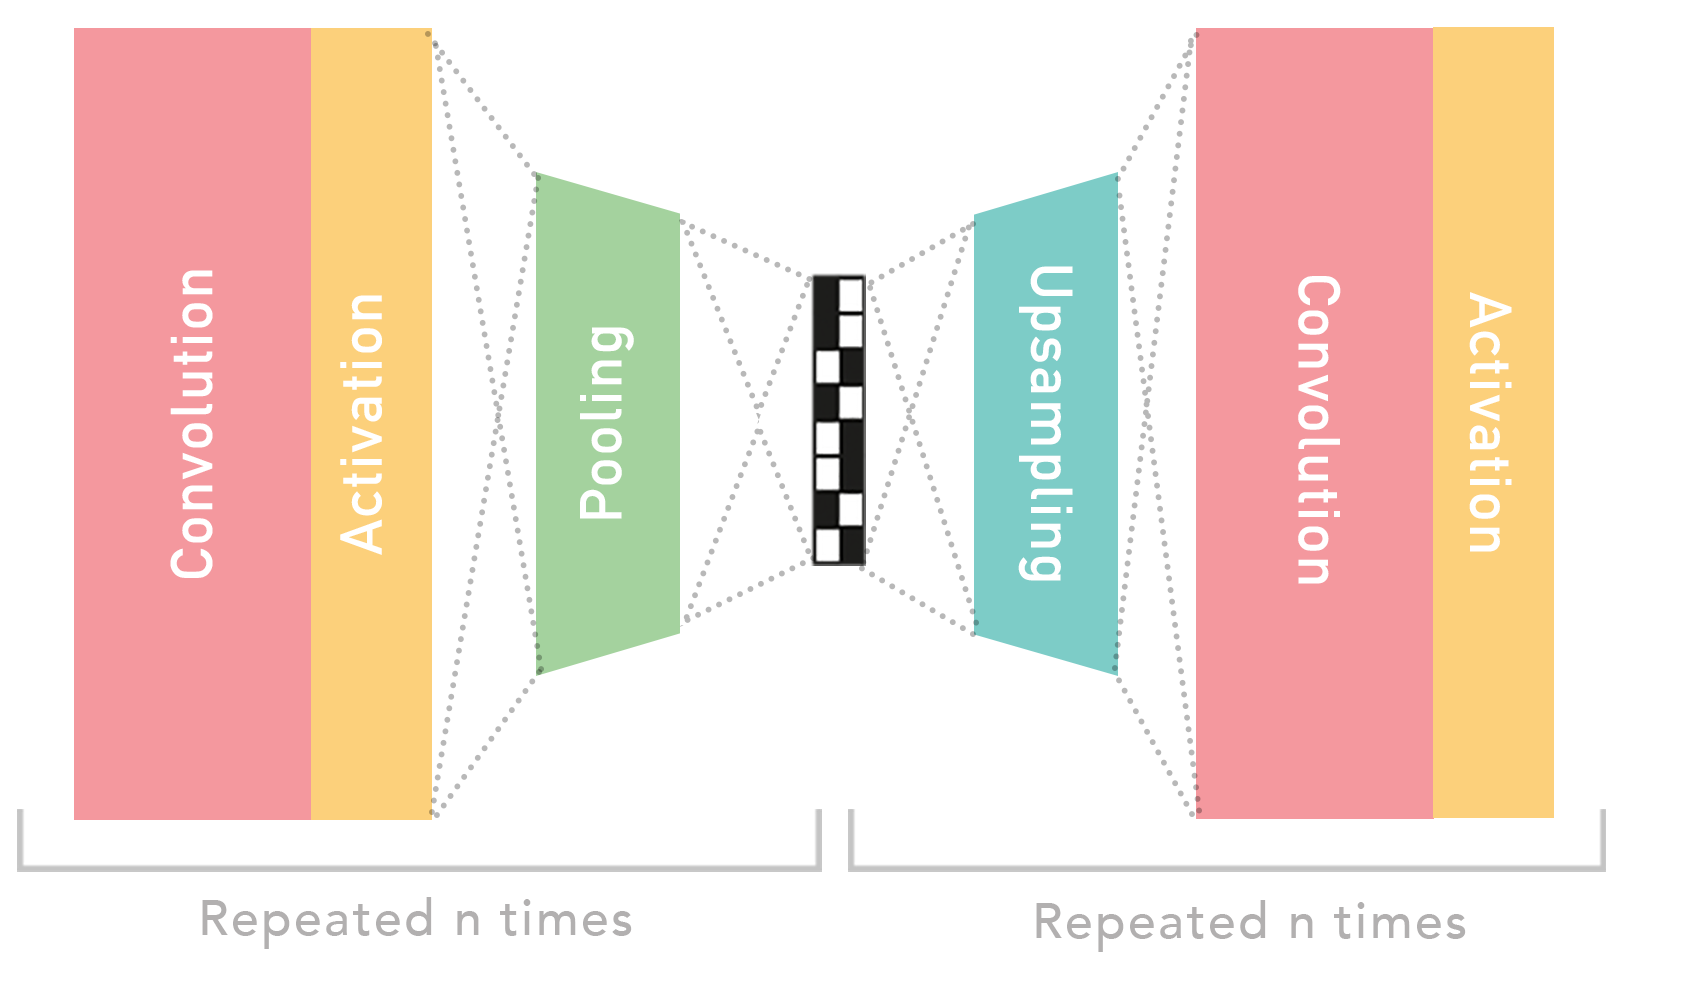
\includegraphics[width=0.6\textwidth]{dissertation/figures/autoencoder_repeat_structure.png}
    \caption{Diagram for a typical autoencoder structure. Operations are symmetrical for the input to be reconstructed with the same dimensions at the output.}
    \label{fig:symmstruc}
\end{figure}

\textit{Convolution} refers to the process of taking the weighted sums of neighbouring values. Put another way, convolutional layers can be thought as a window sliding over an image and summing everything within that window. The specific behaviour of a convolution operation is determined by the filter it uses. Each element in the window will be multiplied by the corresponding element of the filter. We can specify both how big the filter should be, as well as how many different filters should be used. If we use 64 filters, we will learn 64 features about the image, but it will also multiply our dimensions by 64. Figure \ref{fig:convolution} illustrates the convolution process.

\begin{figure}[h]
    \centering
    \missingfigure[]{}
    \caption{Step-by-step illustration of a simple convolution operation on a 4x4 image with a 2x2 kernel. Adapted from Dumoulin and Visin, 2016 (\cite{https://github.com/vdumoulin/conv_arithmetic})}
    \label{fig:convolution}
\end{figure}

\textit{Activation functions} define whether or not each element in the output of the convolutional layer (in this case) should be set to `on' or `off' i.e. whether it should be activated. The purpose of an activation function is to only keep elements of the hidden layers' outputs if it seems to be contributing to the learning of the model.

\textit{Pooling layers} will downsample an image by passing a window over an image and selecting a set value from that window as the one to keep. There are two main types of pooling operations commonly used: average pooling and maximum pooling. In average pooling, the mean value of a window will be chosen as output. In maximum pooling, the maximum value of a window will be chosen. Their counterpart are \textit{upsampling layers} which will resize an image to the right dimensions for a convolutional operation to be applied to it. An illustration of the how these layers function is provided in Figure \ref{fig:sampling}. Using a combination of upsampling and convolutional layers is an alternative to using deconvolution layers which have the drawback of creating checkerboard artifacts (Odena et al., 2016 \cite{https://distill.pub/2016/deconv-checkerboard/})

%https://www.oreilly.com/library/view/deep-learning-for/9781788295628/467cf02b-dc52-49c5-9289-b2721f6758da.xhtml
% http://cs231n.github.io/convolutional-networks/#pool
\begin{figure}[h]
    \centering
    \missingfigure[]{}
    \caption{Left: maximum pooling of 2x2 with stride of 2 applied to a 4x4 image. The image is reduced by a factor of 2. Right: upsampling Right: upsampling of 2x2 with stride of 2 applied to a 2x2 image. The image is augmented by a factor of 2. Adapted from (\cite{http://cs231n.github.io/convolutional-networks/#conv})}
    \label{fig:sampling}
\end{figure}

Throughout the development of the autoencoder, the aim was to maximise the reduction of dimensionality while maintaining a satisfactory reconstructed image. A trade-off had to be done. Size of the coded representation was mainly impacted by the number of hidden layers and size of the convolution and pooling filters. Quality of the reconstructed image could be improved with larger features being used in the convolutional layers and smaller filters.

\bigskip
\subsubsection{Implementation choices}
\hfill
\hfill

Knowing this, the structure of the autoencoder was tuned by trial and error and literature review of existing neural networks for other applications.

In order to avoid losing too much detail in the reconstructed image, we only used 3x3 filters in convolution layers and pooling was done by a factor of 2. Moreover, we kept the number of filters in convolution layers relatively high so as not to lose too much detail in the images. Our structure also used decreasing filter size instead of increasing filter size. Even though increasing filter size showed slight improvements in reconstruction, they are minimal, and having bigger filters towards the bottleneck layer generated bigger coded dimensions. We also decided to replace the pooling operation in the last layer before the bottleneck by a strided convolution layer, because our experiments showed that the colours in the reconstructed image seemed slightly brighter when using striding over pooling (see Figure \ref{}).

In the hidden layers, the choice of activation function was a variant of the Rectified Linear Unit (ReLU), Parametric Rectified Linear Unit (PReLU). ReLU simply returns 0 if the weight unit in the output of a layer is less than 0, or the actual weight if it is bigger than 0. It has become popular because it has been shown to outperform the conventional sigmoid function (\cite{V. Nair and G. E. Hinton. Rectified linear units improve
restricted boltzmann machines. In ICML, pages 807–814,
2010.}, \cite{X. Glorot, A. Bordes, and Y. Bengio. Deep sparse rectifier
networks. In Proceedings of the 14th International Conference on Artificial Intelligence and Statistics, pages 315–323,
2011.}), as well as helping with faster training convergence (\cite{A. Krizhevsky, I. Sutskever, and G. Hinton. Imagenet classification with deep convolutional neural networks. In NIPS,
2012.}). PReLU differs from ReLU by having a small slope for negative values which means it does not map all negative values to 0. This slope is made a learning parameter and is determined by the neural network during training. Figure \ref{relu_prelu} illustrates the difference between the two. He et al., 2015 (\cite{https://arxiv.org/pdf/1502.01852.pdf}) showed that PReLU can improve model fitting for image classification applications. Reconstruction difference using PReLU over ReLU in our network is shown in Figure \ref{}.

\begin{figure}[h]
    \centering
    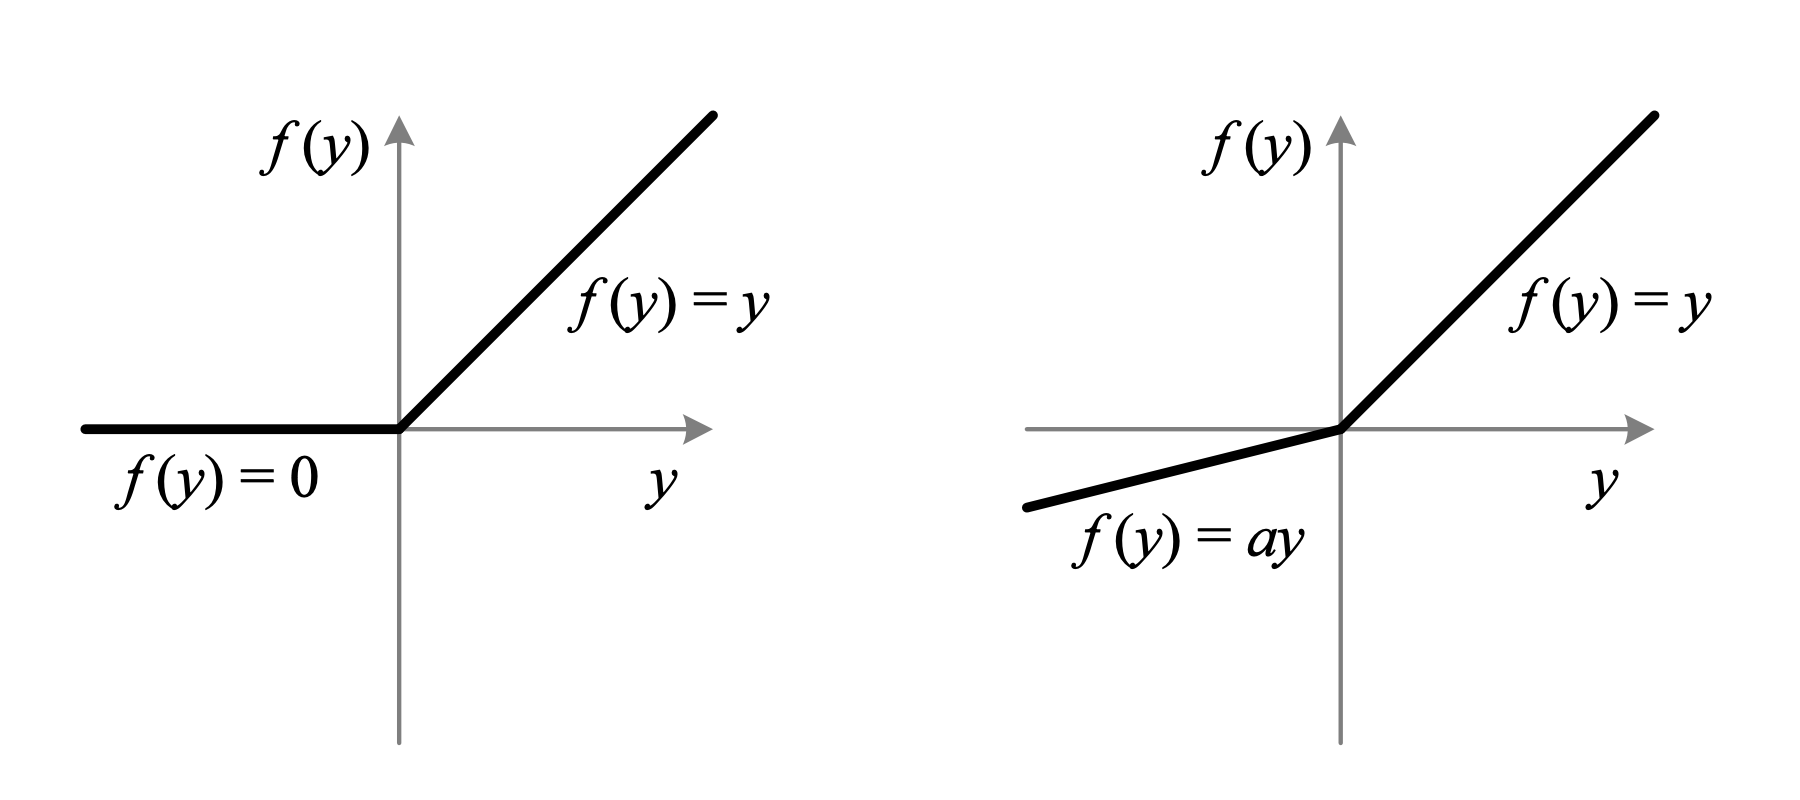
\includegraphics[width=.6\textwidth]{dissertation/figures/relu_prelu.png}
    \caption{[TODO improve] ReLU (left) vs. PReLU (right). The negative part of the PReLU function is variable and a parameter to be learned. Source: He et al., 2015}
    \label{fig:relu_prelu}
\end{figure}

The activation function at the output of the network was the logistic sigmoid activation function, as we needed to restrict output to the [0, 1] range of our image pixels. Figure \ref{fig:sigmoid} illustrates this activation function.

\begin{figure}[h]
    \centering
    \missingfigure[]{Graph showing the logistic sigmoid function slope as well as the equation.}
    \caption{[TODO caption] Logistic sigmoid function.}
    \label{fig:sigmoid}
\end{figure}

Our final autoencoder structure reduced dimensions by a factor of 2 a total of 5 times, resulting in a ten-fold reduction of dimensions on the original 110,592 pixels. The final coded dimensions were of 1,152. Figure \ref{diff_reconstructions} illustrates how the autoencoder reconstructed an input image depending on number of pooling operations. We traded-off some reconstruction quality in order to obtain a smaller coded dimension in the hope that it would help high-dimensional visualisation algorithms perform better, as well as be a better starting block for a regression model.

\begin{figure}[h]
    \centering
    \missingfigure[]{Show reconstruction performance for 3 hidden layers, 4 layers, 5 layers.}
    \caption{Reconstructed images by the autoencoder according to the size of the coded layer. Left shows the input image, and right shows the output image.}
    \label{fig:diff_reconstructions}
\end{figure}

The autoencoder was training with binary cross-entropy as a loss function, as we are aiming to minimise the difference between two distributions: the input, and the reconstructed output. The final structure of the autoencoder is shown below in Figure \ref{fig:autoencoder_details}. Keras code for building the model is available in Listing \ref{lst:autoencoder}.

\begin{figure}[h]
    \centering
    \missingfigure[]{Detailed summary graph of the autoencoder model}
    \caption{[TODO caption]}
    \label{fig:autoencoder_details}
\end{figure}

\subsection{Deep regression}

The regression model was built on the encoder part of the autoencoder. We wanted to use the dimensionality reduction capacities of the encoder layers to evaluate whether interaction could be quantified from an image's feature vector.

The structure of the regression model was kept simple. Research reviewing existing general-purpose neural networks such as VGG-16 showed that adequate tuning of these models obtained results close to `state-of-the-art' without having to resort to more complicated structures. We did not reuse such a general purpose model but the convolutional part of the VGG-16 network is similar to the decoder part of our autoencoder, using 5 combinations of convolutions and pooling operations (Simonyan and Zisserman, 2015). These operations are followed by a small number of fully-connected layers. Hence, we decided to follow this template and not make our regression structure overly complex.

The encoder model was extracted from the autoencoder with the bottleneck layer flattened. This encoder model was then extended with two fully connected layers separated by a dropout layer. Dropout has shown to make models more robust and prevent overfitting (Hinton et al., 2012). The final regression predictions were outputted with a fully connected layer of size 1, activated by a linear function.

The choice of the linear function was justified by the following. The input to the regression model was 192x192x3 images accompanied with labels in the range [0, 100] representing a percentage of overlap between two groups of cells. As such, we want the output activation function to be limited to [0, 100]. Both softplus and linear activations were candidates. The linear activation had to be used with a non-negative kernel constraint, as overlap percentage cannot be negative but the linear function normally allows for negative values. The softplus activation function outputs values in the range [0, $+\infty$]. Performance in terms of training loss was similar, however the linear function performed overall better. Furthermore, softplus does not map an input to itself (shown in Figure \ref{}) and is harder to differentiate compared to the linear function, which would make training slower.

\begin{figure}[h]
    \centering
    \missingfigure[]{Graphs comparing the linear and softplus function.}
    \caption{[TODO caption] Linear function (left) vs. softplus function (right).}
    \label{fig:sigmoid}
\end{figure}

The regression model was trained with mean-squared-error loss, which calculates the difference between the predictions of the model and the truth values of the labels. The final structure of the deep regression model is shown below in Figure \ref{fig:regression_details}. Keras code for building the model is available in Listing \ref{lst:regression}.

\begin{figure}[h]
    \centering
    \missingfigure[]{Detailed summary graph of the regression model}
    \caption{[TODO caption]}
    \label{fig:regression_details}
\end{figure}

\chapter{Evaluation} 

\section{Methodology}

This section will evaluate the performance of our autoencoder and regression models on unseen images. As explained in Section \ref{subsec:selecting_dataset}, three sets of images were selected for research:

\begin{itemize}
    \item A \textbf{full dataset} containing all categories, with no class imbalance issues
    \item A \textbf{dual dataset}, with no class imbalance issues, containing images from two classes only 
    \item A `\textbf{DMSO-only' dataset}, which should show the most distinction between classes, with class imbalance issues. This dataset did not include any experimental conditions using drugs, only stimulation conditions.
\end{itemize}

Each image in these datasets was categorised by stimulation level: one of \textit{Unstimulated}, \textit{OVA}, or \textit{ConA}. If the image contained image aberrations, it was labelled \textit{Faulty} instead in the case of the autoencoder. In the case of the regression model, the overlap value of \textit{Faulty} images was set to 0. Figure \ref{fig:explain_categories} illustrates what an image from each category looks like.

\begin{figure}[h]
    \centering
    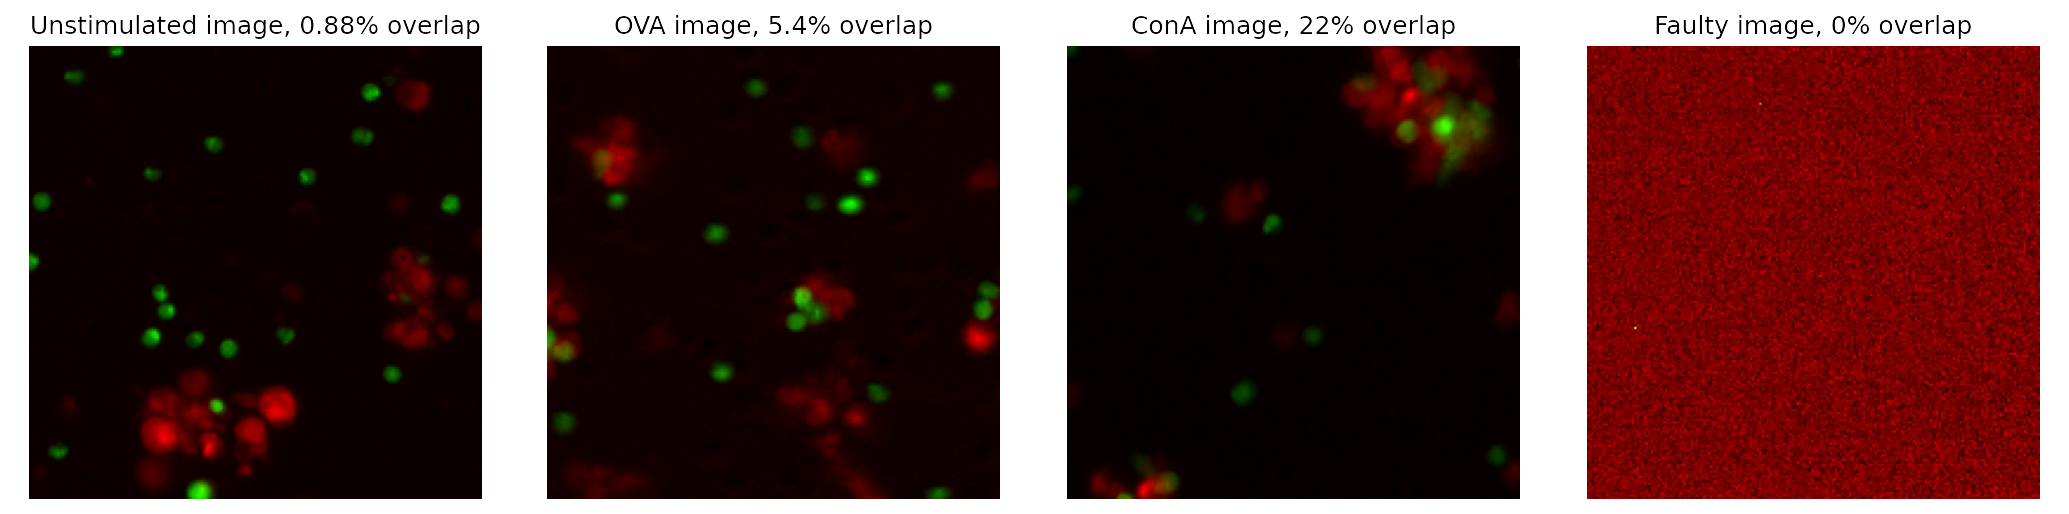
\includegraphics[width=\textwidth]{dissertation/figures/category_images.png}
    \caption{Example validation images taken from each stimulation category. Each image is also labelled with its overlap value. From left to right: \textit{Unstimulated}, $0.88\%$ overlap; \textit{OVA}, $5.4\%$; \textit{ConA}, $22\%$; \textit{Faulty}, $0\%$.}
    \label{fig:explain_categories}
\end{figure}

We had two versions of each dataset: one which had been noise-corrected, and one which had been background-corrected through the help of k-means colour segmentation. This dataset was denominated the `masked' dataset. We trained separate models on those two datasets to evaluate the impact of the background on the model's learning. 

Training and validating was done on the full dataset's 19,000 instances. We had 10,000 instances of this dataset left for testing, and 13,800 instances of the dual dataset, as well as 8,000 instances of the DMSO dataset. All datasets were consistently shuffled before training and testing with the same random state parameter. We made sure there was no overlap between any of the datasets. No image was used for both training and testing. 

The following criteria were chosen in our evaluation:

\begin{itemize}
    \item The success of the autoencoder model will be evaluated on its capacity at image reconstruction, as well as if a UMAP projection of the coded images shows some underlying structure of the data. 
    \item The regression model will be evaluated on how well it predicts overlap values for unseen images of immune cells. 
\end{itemize}

\section{Autoencoder}

\subsection{How well can we reconstruct an image?}

Our autoencoder model is trained on binary cross-entropy loss. The model learns by trying to minimise the difference between two distributions of pixels: the input, and the output. The closer the loss is to 0, the more similar the two distributions are. This means that a score closer to 0 is equivalent to the autoencoder reconstructing an image well. We can use this value as a metric for comparing results between models and datasets. We can also assess the visual quality of an image on reconstruction. 

The following images in Figures \ref{fig:full_reconstruction}, \ref{fig:dual_reconstruction}, \ref{fig:dmso_reconstruction} show how the autoencoder performed on image reconstruction for each of the datasets. The output images were all reconstructed by the model from a 1,152 inner representation of the input image of 110,592 pixels.

\begin{figure}[h!]
    \centering
    \begin{subfigure}[h!]{0.45\textwidth}
        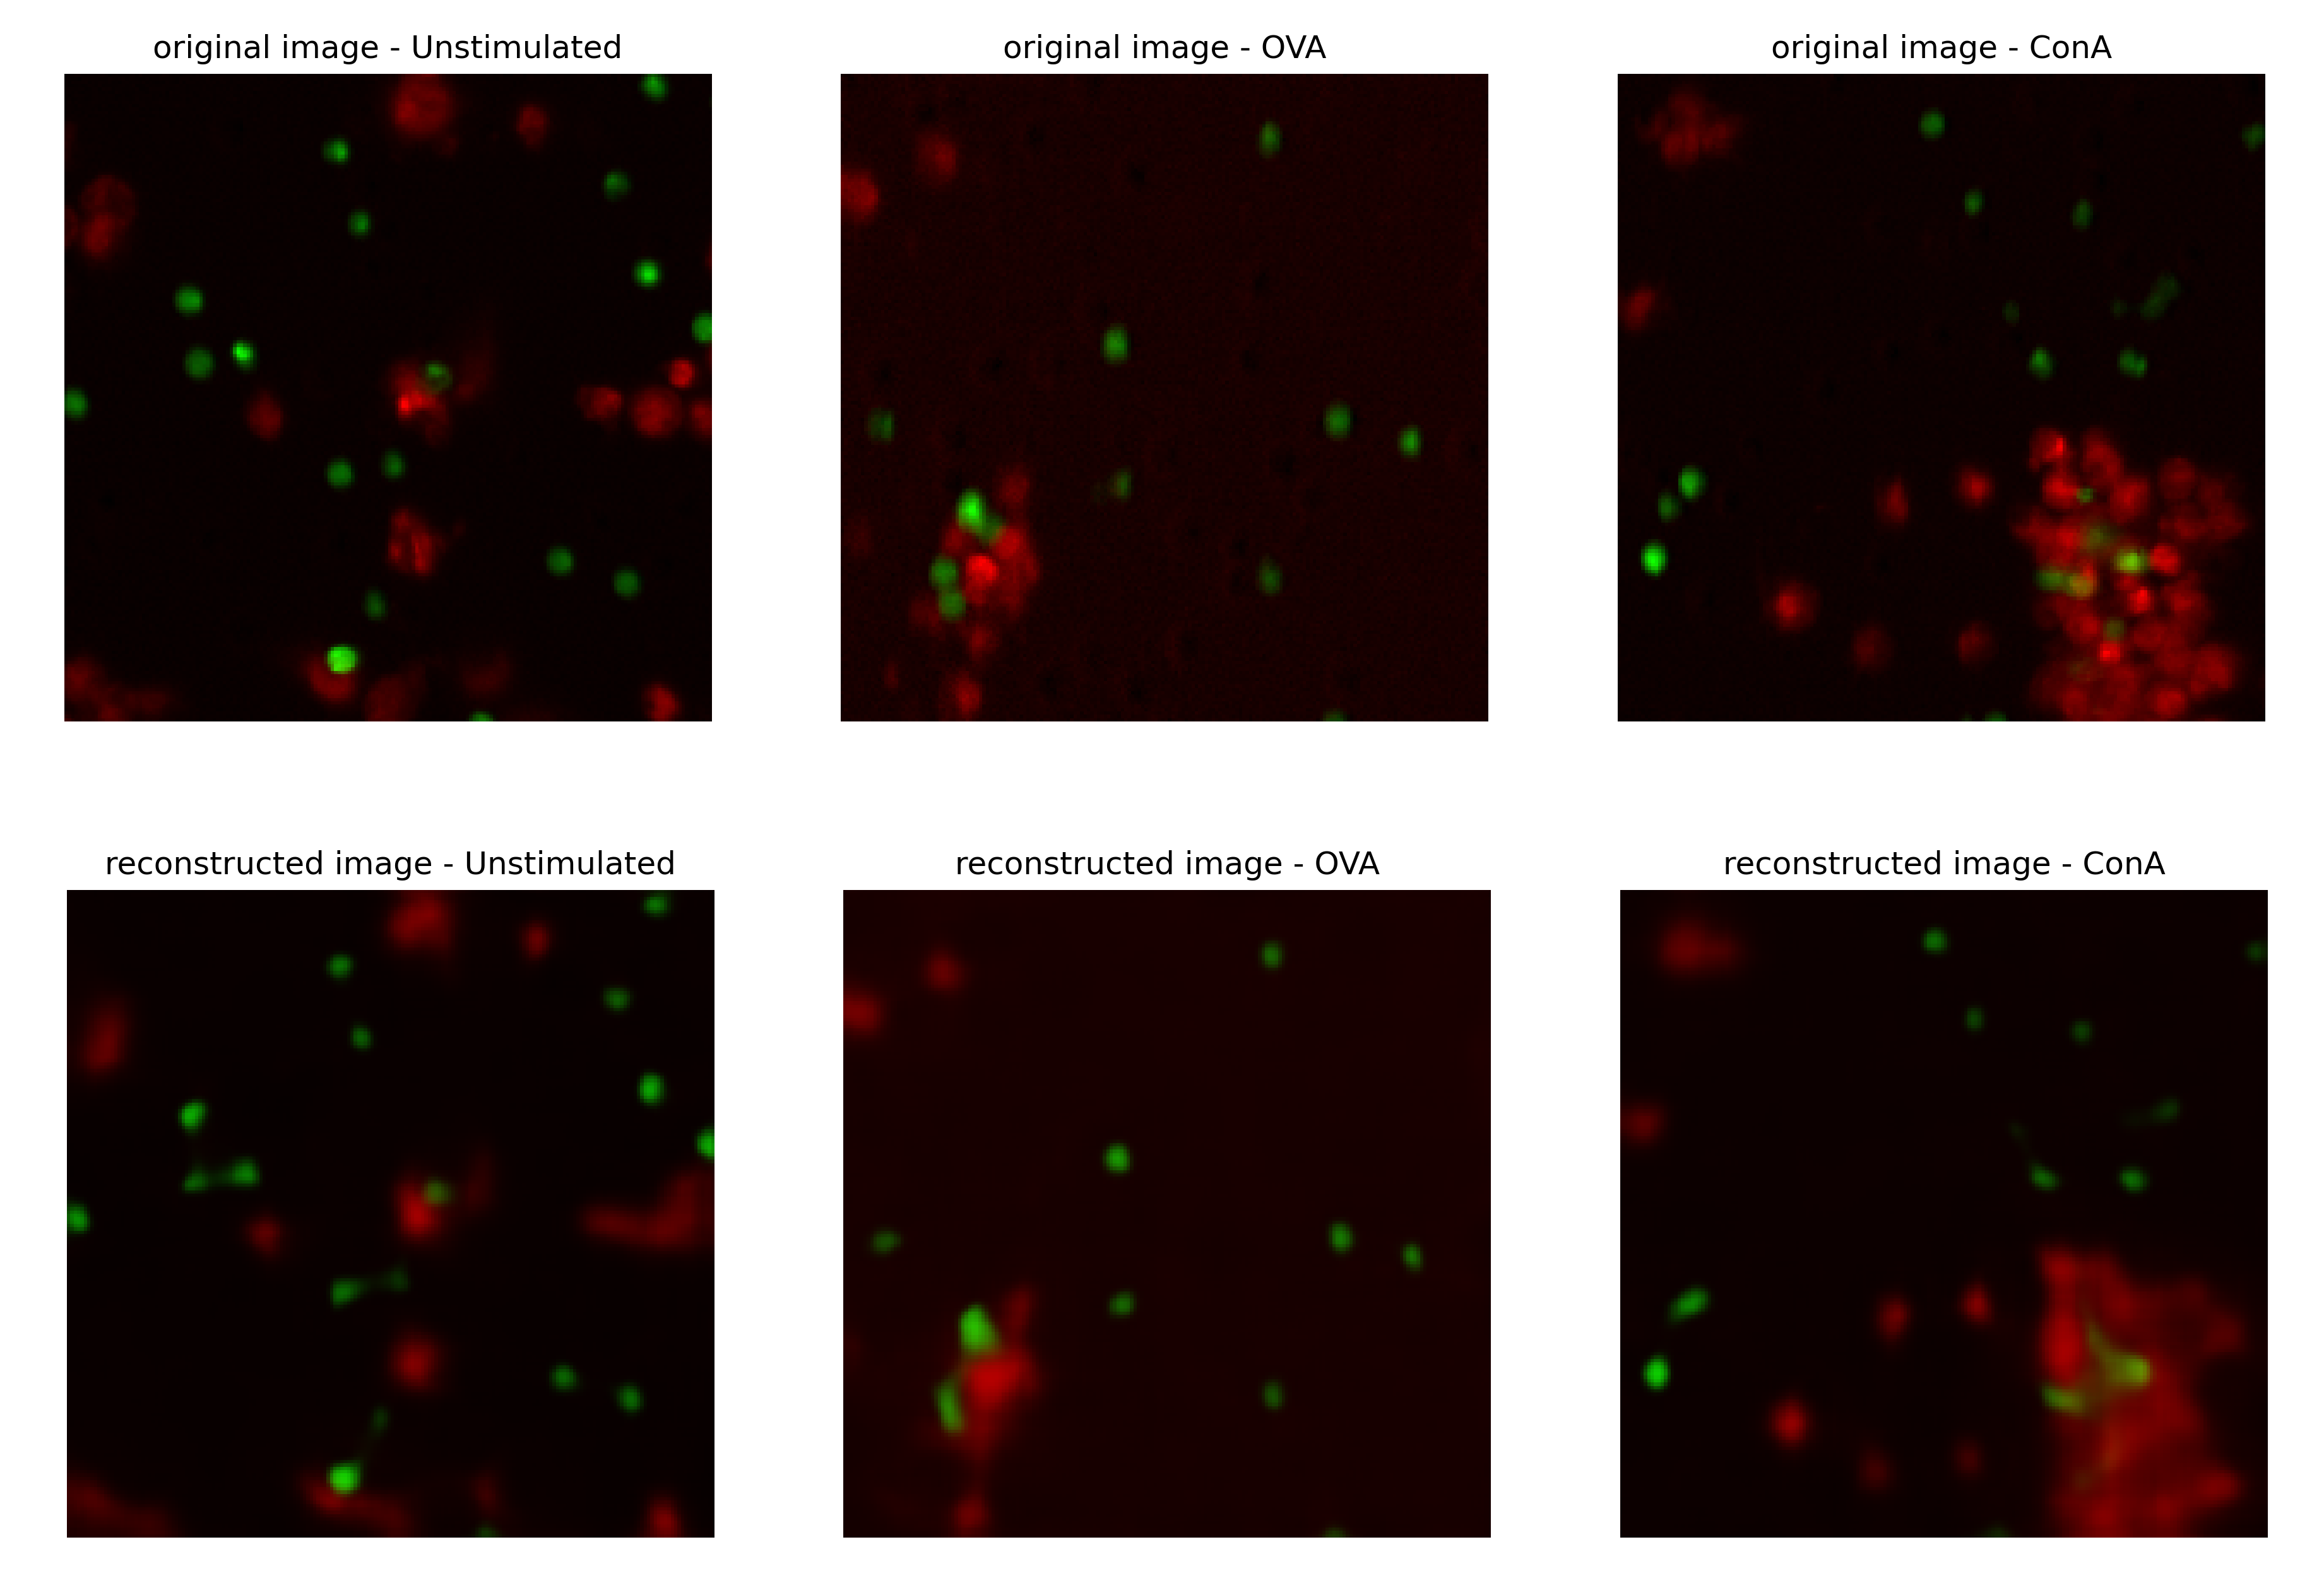
\includegraphics[width=\textwidth]{dissertation/figures/evaluation/CK19_reconstruction.png}
        \caption{Normal images}
    \end{subfigure}
    \begin{subfigure}[h!]{0.45\textwidth}
        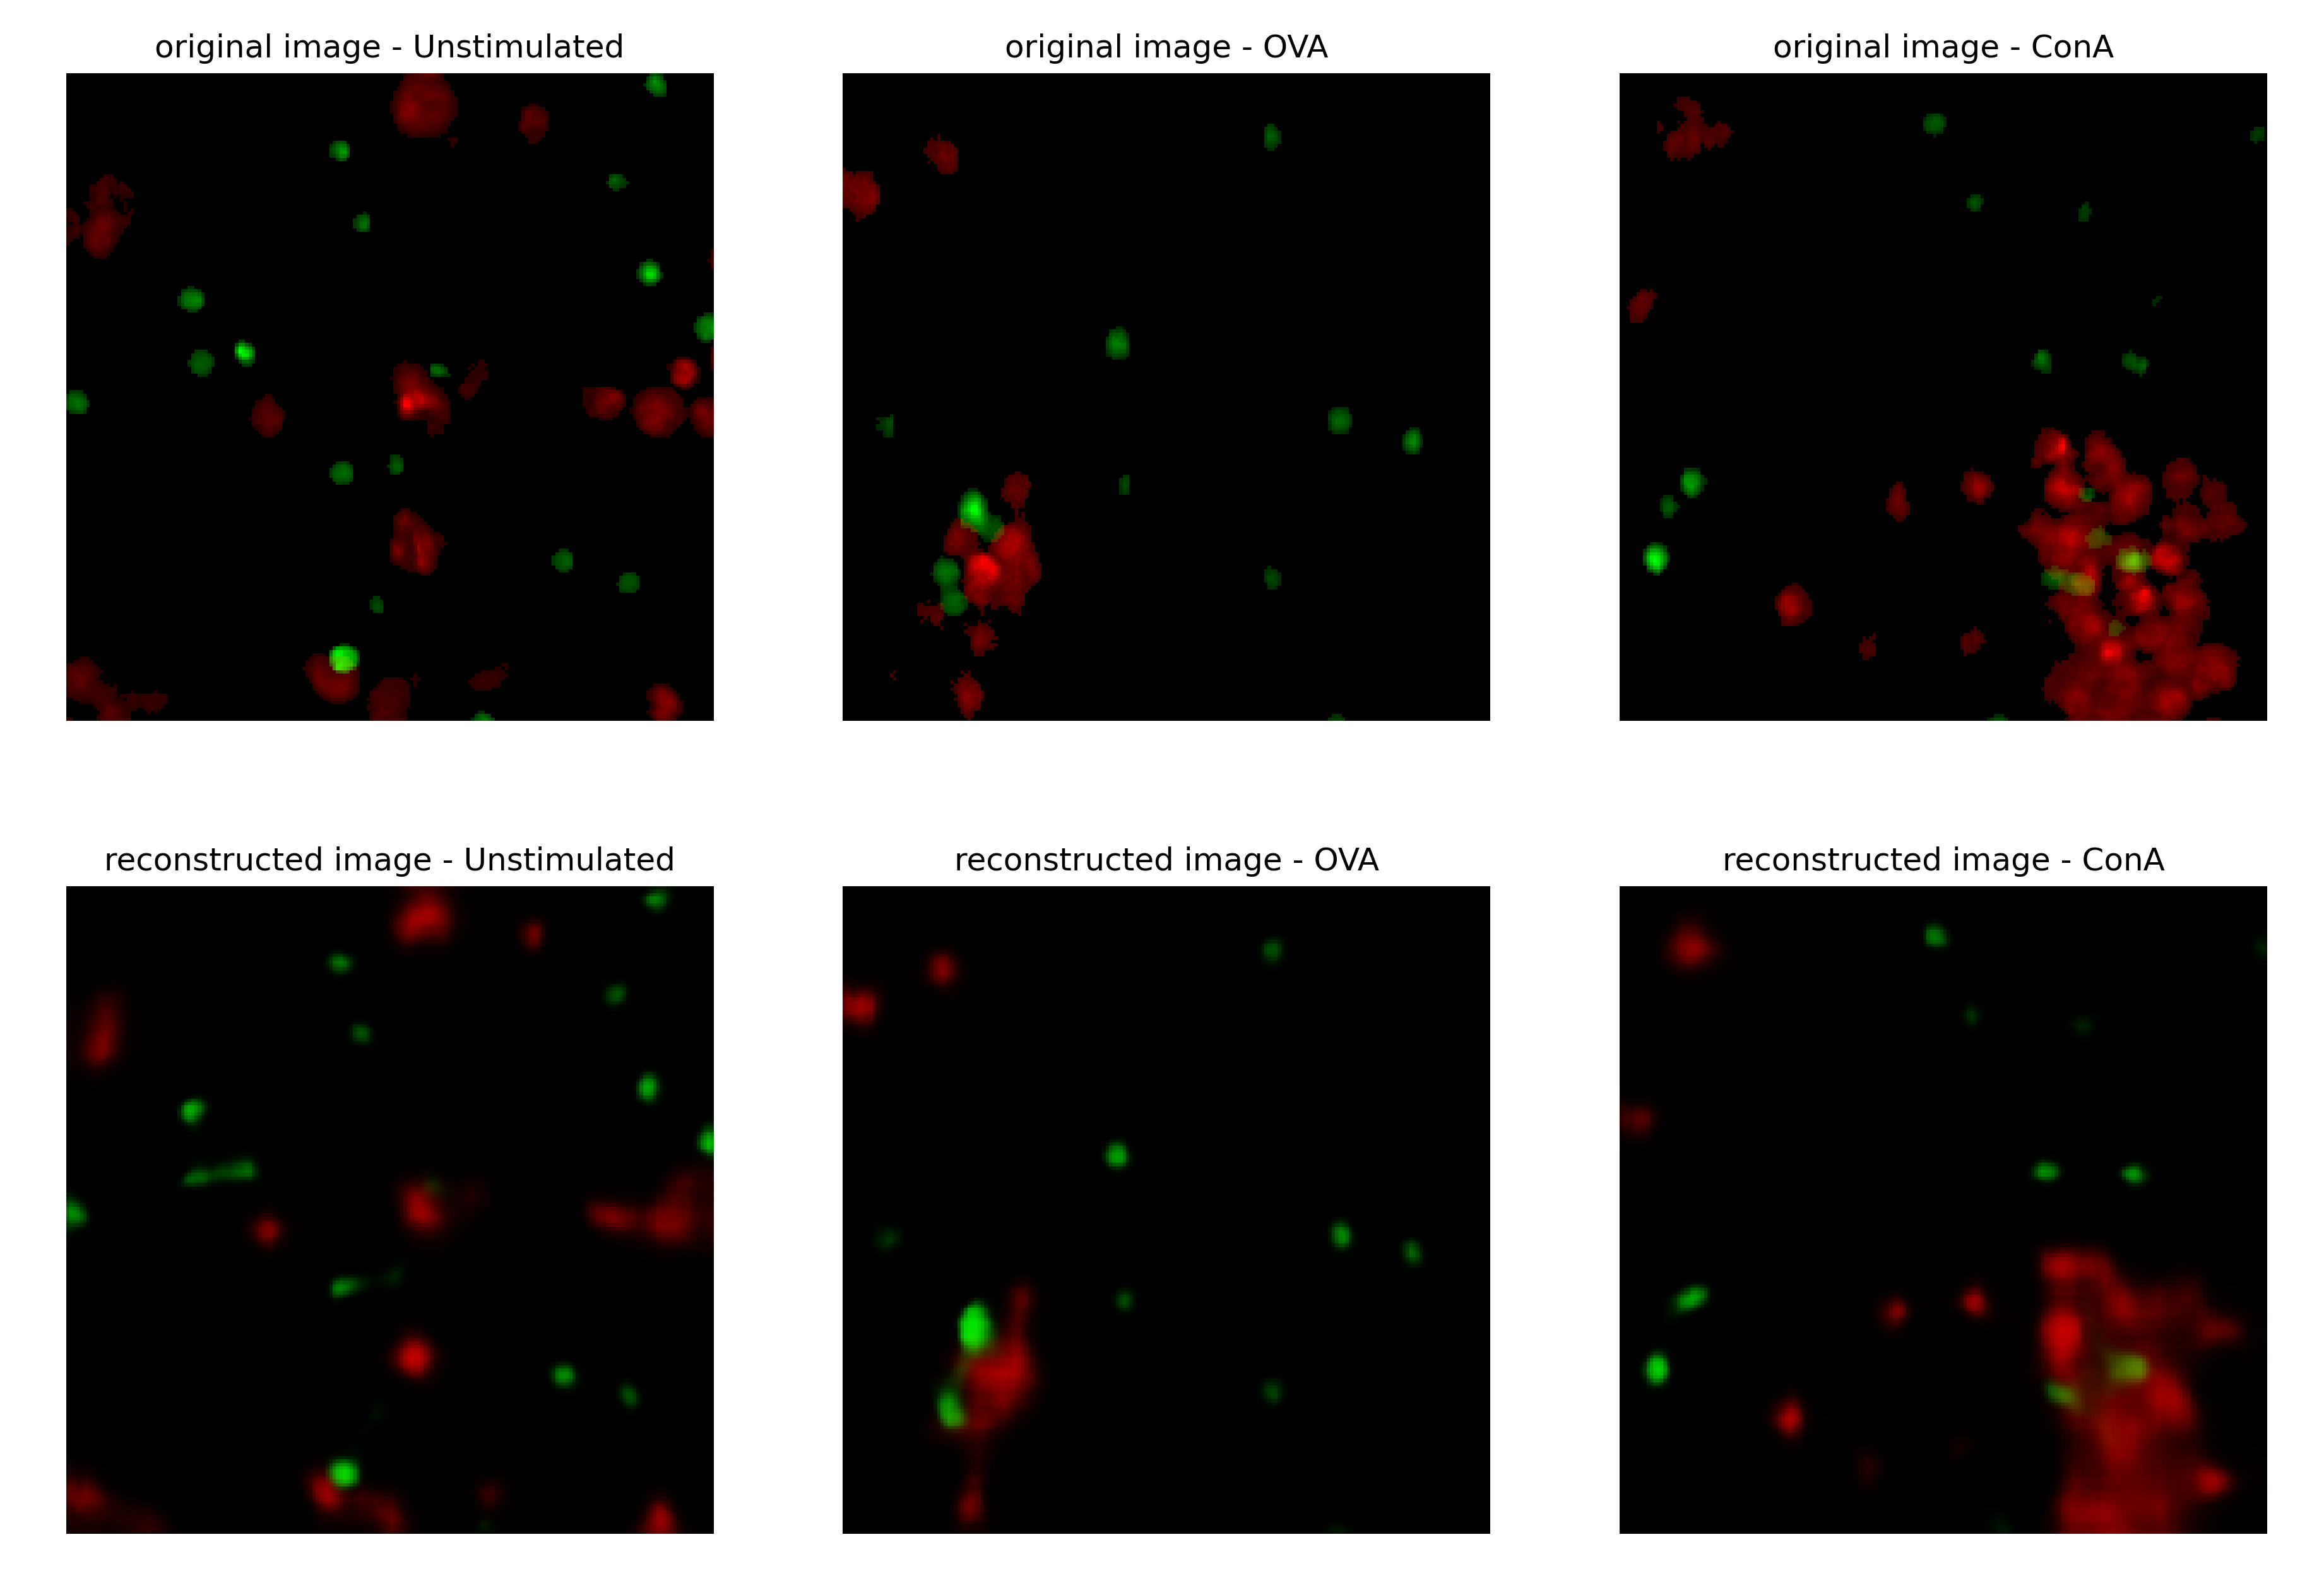
\includegraphics[width=\textwidth]{dissertation/figures/evaluation/CK19_masked_reconstruction.png}
        \caption{Masked images}
    \end{subfigure}
    \caption{Autoencoder-reconstructed images from the test images of \textbf{full} dataset. For each of the subfigures, categories are Unstimulated, OVA, ConA from left to right. Input images are at the top, and reconstructed images at the bottom.}
    \label{fig:full_reconstruction}
\end{figure}

\begin{figure}[h!]
    \centering
    \begin{subfigure}[h!]{0.3\textwidth}
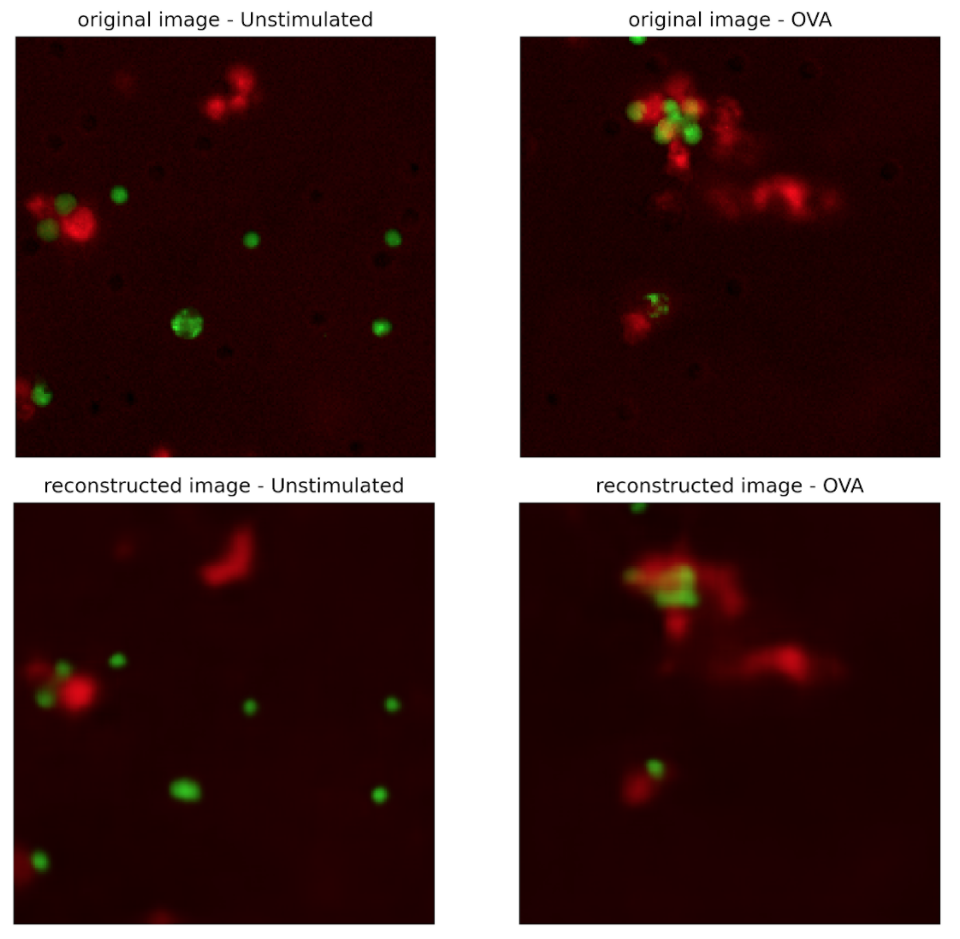
\includegraphics[width=\textwidth]{dissertation/figures/evaluation/CK22_reconstruction.png}
        \caption{Normal images}
    \end{subfigure}
    \begin{subfigure}[h!]{0.3\textwidth}
        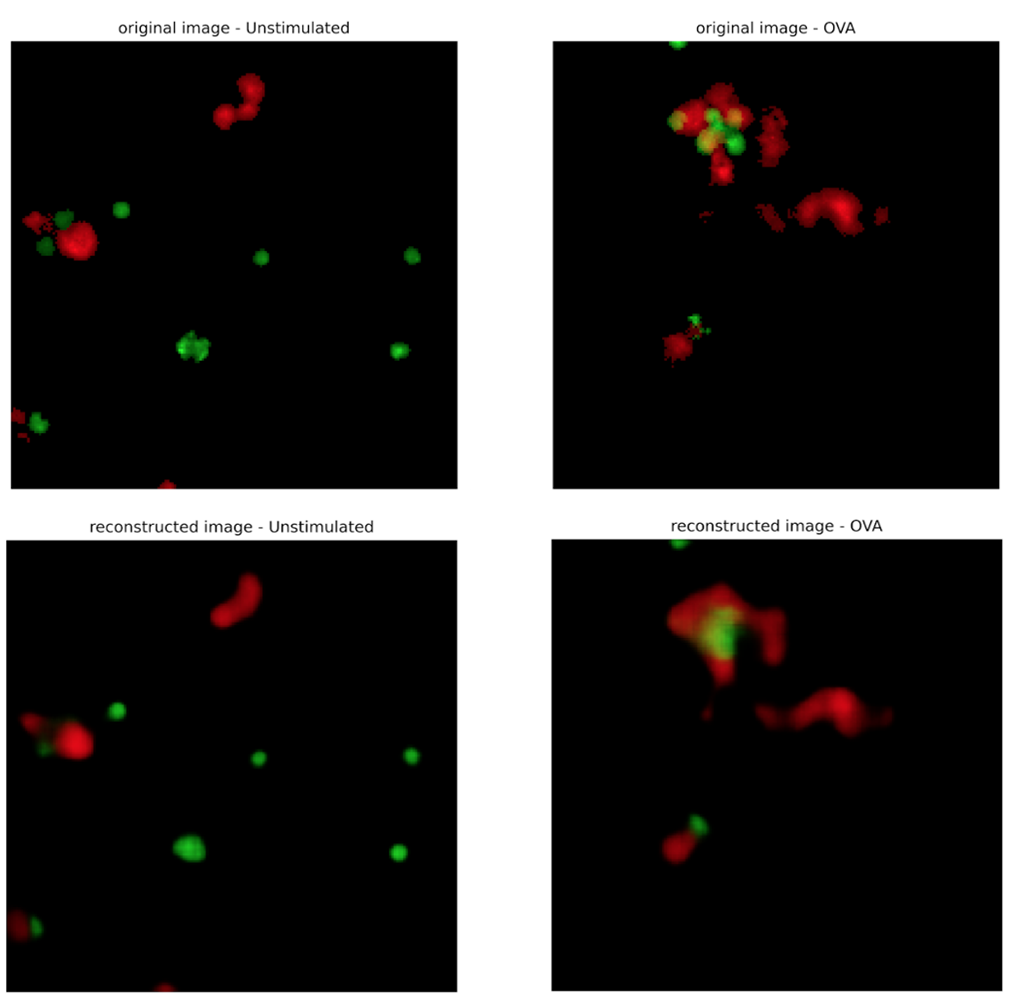
\includegraphics[width=\textwidth]{dissertation/figures/evaluation/CK22_masked_reconstruction.png}
        \caption{Masked images}
        \label{fig:dual_masked_recon}
    \end{subfigure}
    \caption{Autoencoder-reconstructed images from the \textbf{dual} dataset. For each of the subfigures, stimulation categories are Unstimulated (left) and OVA (right). Input images are at the top, and reconstructed images at the bottom.}
    \label{fig:dual_reconstruction}
\end{figure}

\begin{figure}[h!]
    \centering
    \begin{subfigure}[h!]{0.45\textwidth}
        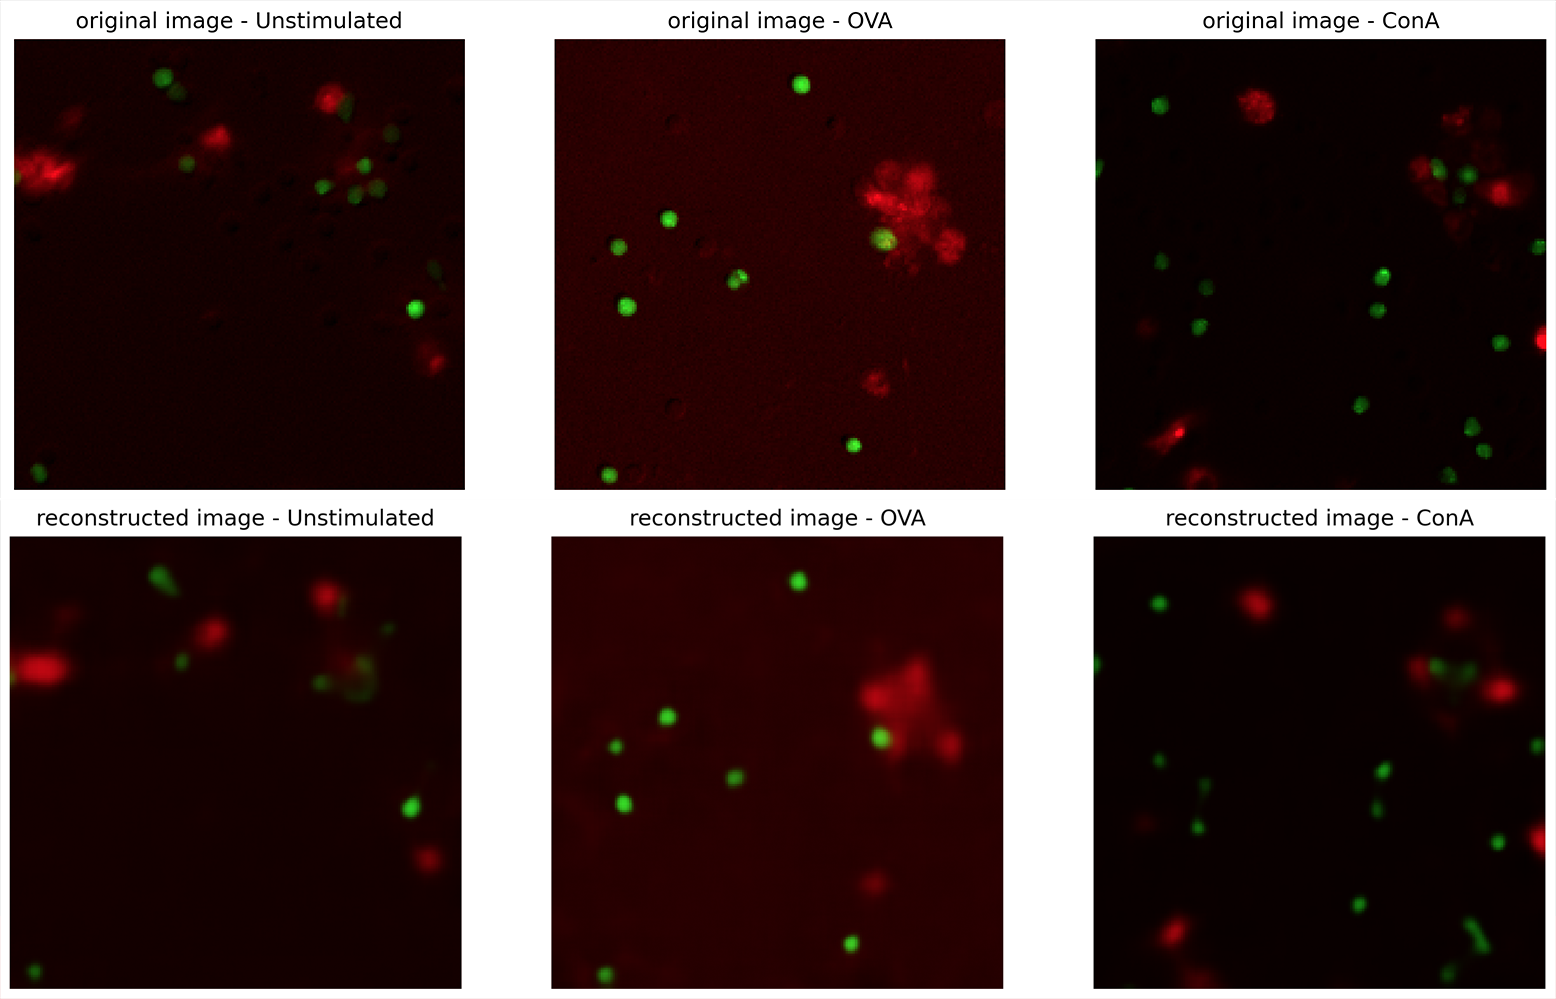
\includegraphics[width=\textwidth]{dissertation/figures/evaluation/DMSO_reconstruction.png}
        \caption{Normal images}
    \end{subfigure}
    %
    \begin{subfigure}[h!]{0.46\textwidth}
        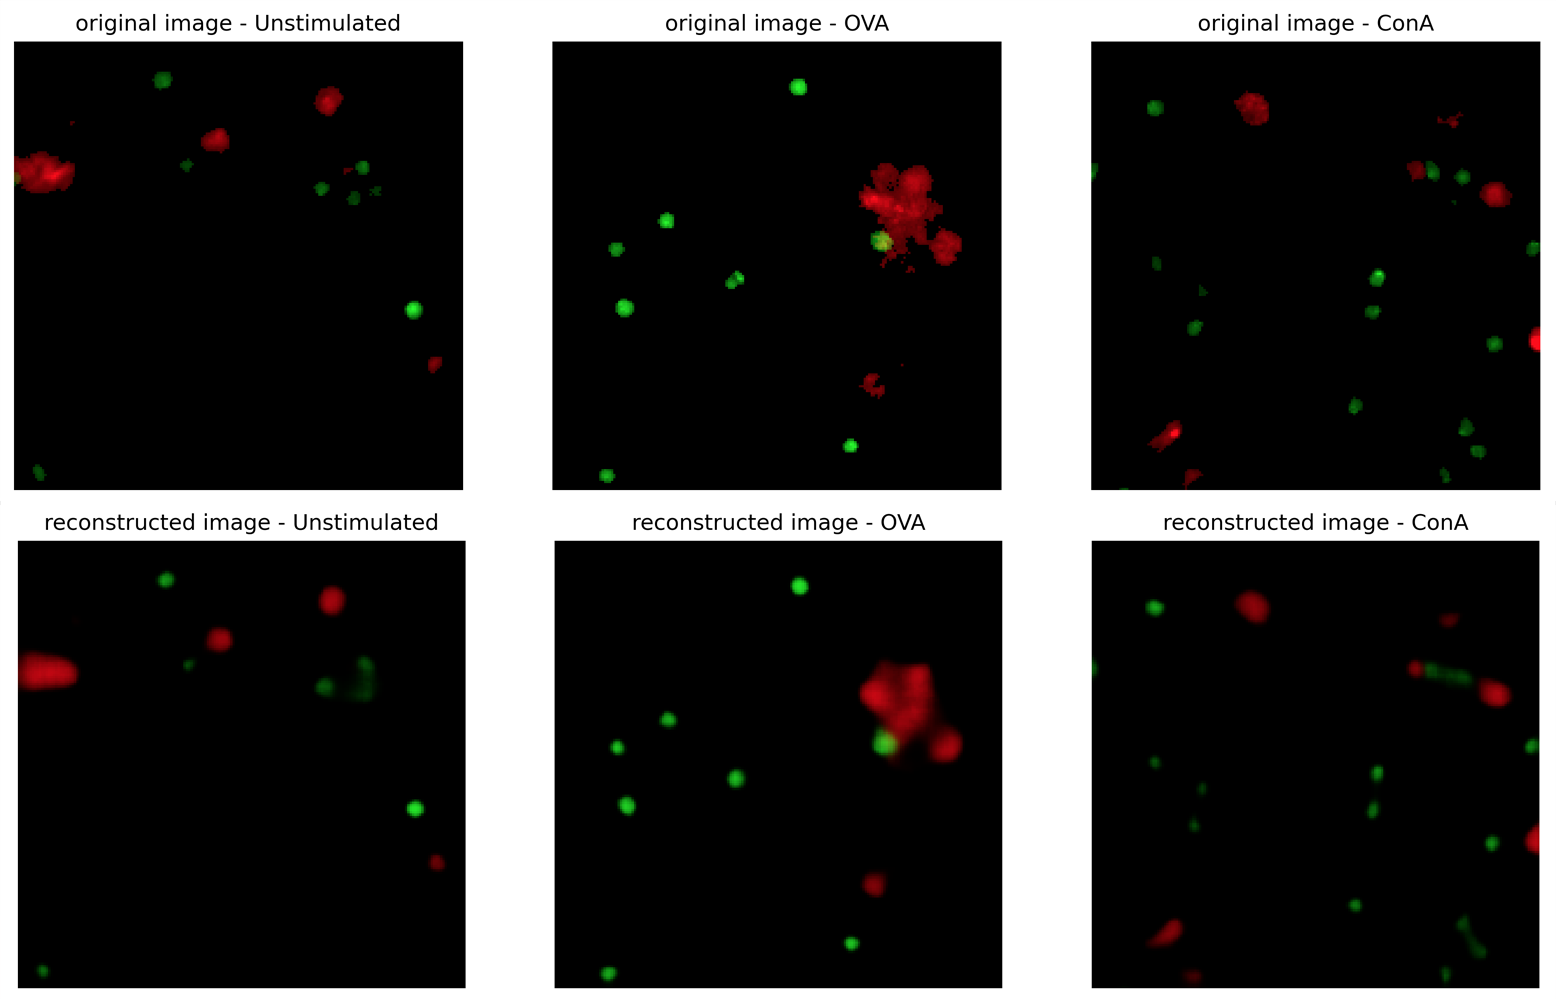
\includegraphics[width=\textwidth]{dissertation/figures/evaluation/DMSO_masked_reconstruction.png}
        \caption{Masked images}
        \label{fig:dmso_masked_recon}
    \end{subfigure}
    \caption{Autoencoder-reconstructed images from the \textbf{DMSO} dataset. For each of the subfigures, categories are Unstimulated, OVA, ConA from left to right. Input images are at the top, and predicted images at the bottom.}
    \label{fig:dmso_reconstruction}
\end{figure}

The main feature we can note from these images is that visually, the autoencoder reconstructed the images in quite a satisfactory way – we can still see where cells are and where they overlap. We can recognise the images's similarities. We can also identify some flaws. The main drawback of the autoencoder model is the way it merges different cells together, creating `blobs' rather than more detailed cell objects.

On the other hand, we can note that the masked autoencoder trained on the masked images of immune cells achieve a higher level of detail, for all datasets. Particularly, the images reconstructed by the masked model retain the circularity of the cell objects better, even in the unseen datasets. This can be observed in Figures \ref{fig:dual_masked_recon} and \ref{fig:dmso_masked_recon} where the dendritic cells in red hold their original shape and detail better in comparison to their non-masked counterpart.

Visually, it is not immediately clear how much better the autoencoder performs on the full dataset, part of which it has seen, compared to the unseen dual and DMSO datasets. Indeed, we will not be able to fully compare the reconstruction of these images by eye. Further to visual evaluation of the reconstruction of the immune cells, the two models's prediction losses can provide another perspective on their performance. Table \ref{tab:autoencoder_loss} reports loss values for each model on each dataset.

\begin{table}[!h]
\centering
\caption{Binary cross-entropy loss value for the autoencoder models's performances on each of the test datasets. A value closer to 0 is better. We can observe a gain in performance across datasets in the masked model.}
\label{tab:autoencoder_loss}
\begin{tabular}{l|r|r|r}
\rowcolor[HTML]{EFEFEF} 
Model  & Full   & Dual   & DMSO   \\ \hline
Normal & 0.0870 & 0.1159 & 0.0936 \\ \hline
Masked & 0.0156 & 0.0174 & 0.0166 \\
\end{tabular}
\end{table}

From this data we can say that removing noisy backgrounds entirely from the images of immune cells achieved substantial improvements. It also made the autoencoder's performance on unseen datasets more comparable to the full dataset.

\subsection{Can we find an underlying structure in the images of immune cells?}

While we have shown that an autoencoder can complete the task of reducing the dimensionality of an image of immune cells and reconstruct it fully from this reduced image, we want to look at whether or not this would help with a two-dimensional projection of the datasets. The aim for two-dimensional visualisation of the datasets was that it would allow us to uncover clusters of images grouped around the same stimulation conditions.

Each element projected onto a 2D plane is labelled with one of the \textit{Unstimulated}, \textit{OVA}, \textit{ConA}, or \textit{Faulty} categories at the plotting step.

\bigskip
\subsubsection{Baseline performance}
\hfill
\hfill 

The expectations were that an autoencoder would allow us to extract the necessary features from an image that would be sufficient for it to be reconstructed, but also for it to be analysed. As such, we wanted to compare the visualisation performance of UMAP on the coded images to a baseline performance on raw images that have not been reduced in dimensionality. This was only ran for the full dataset as the large dimensions meant this computation took a considerable amount of time. On a 2015 MacBook Pro with 2.7 GHz i5 core and 8 GB of RAM, running UMAP on the $10,000\times192\times192\times3$ test instances of the full dataset worth took 1 hour, 5 minutes and 33 seconds. The result visualisation is shown in Figure \ref{fig:baseline_vis}.


\begin{figure}[h!]
    \centering
    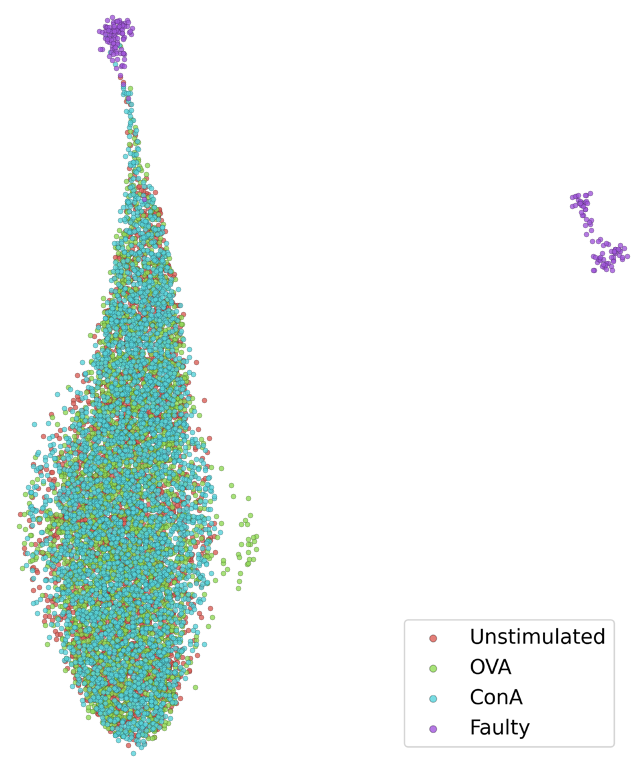
\includegraphics[width=0.45\textwidth]{dissertation/figures/evaluation/CK19_baseline_visualisation.png}
    \caption{Two-dimensional UMAP projection of the 10,000 testing images in the full dataset. UMAP was ran with base parameters $n\_neighbors=15$, $min\_dist=0.1$. The legend highlights which colour corresponds to which stimulation category.}
    \label{fig:baseline_vis}
\end{figure}

This projection highlights that with the raw $192\times193\times3$ images of immune cells, only \textit{Faulty} images seem to be recognised and there is no clear distinction between images of other categories. A few OVA/green points are distanced from the main cluster. We will now look at whether reducing the dimensionality of the images with an autoencoder helps make this distinction.  

\bigskip
\subsubsection{Trained performance}
\hfill
\hfill 

UMAP's speed allowed us to try different parameters for our visualisations to attempt to yield the best projections of the data, as running UMAP only took between 30 seconds and 1 minute and 15 seconds to run on the encoder-processed images. That is an average 75x speedup on the baseline performance.

We can see the projection of the \textbf{full dataset}'s test images in Figure \ref{fig:full_reconstruction}. Two smaller clusters have emerged which were not present in the baseline projection. The labelling shows us that the sparser cluster contains two lines of red/Unstimulated and green/ConA points, which could indicate that the autoencoder did help extract the most important features out of the images. However, the larger cluster still bears no distinction between images of different categories. Furthermore, the projection obtained with the masked model did not seem to perform better, with less clusters being uncovered this way.

\begin{figure}[h!]
    \centering
    \begin{subfigure}[h!]{0.39\textwidth}
        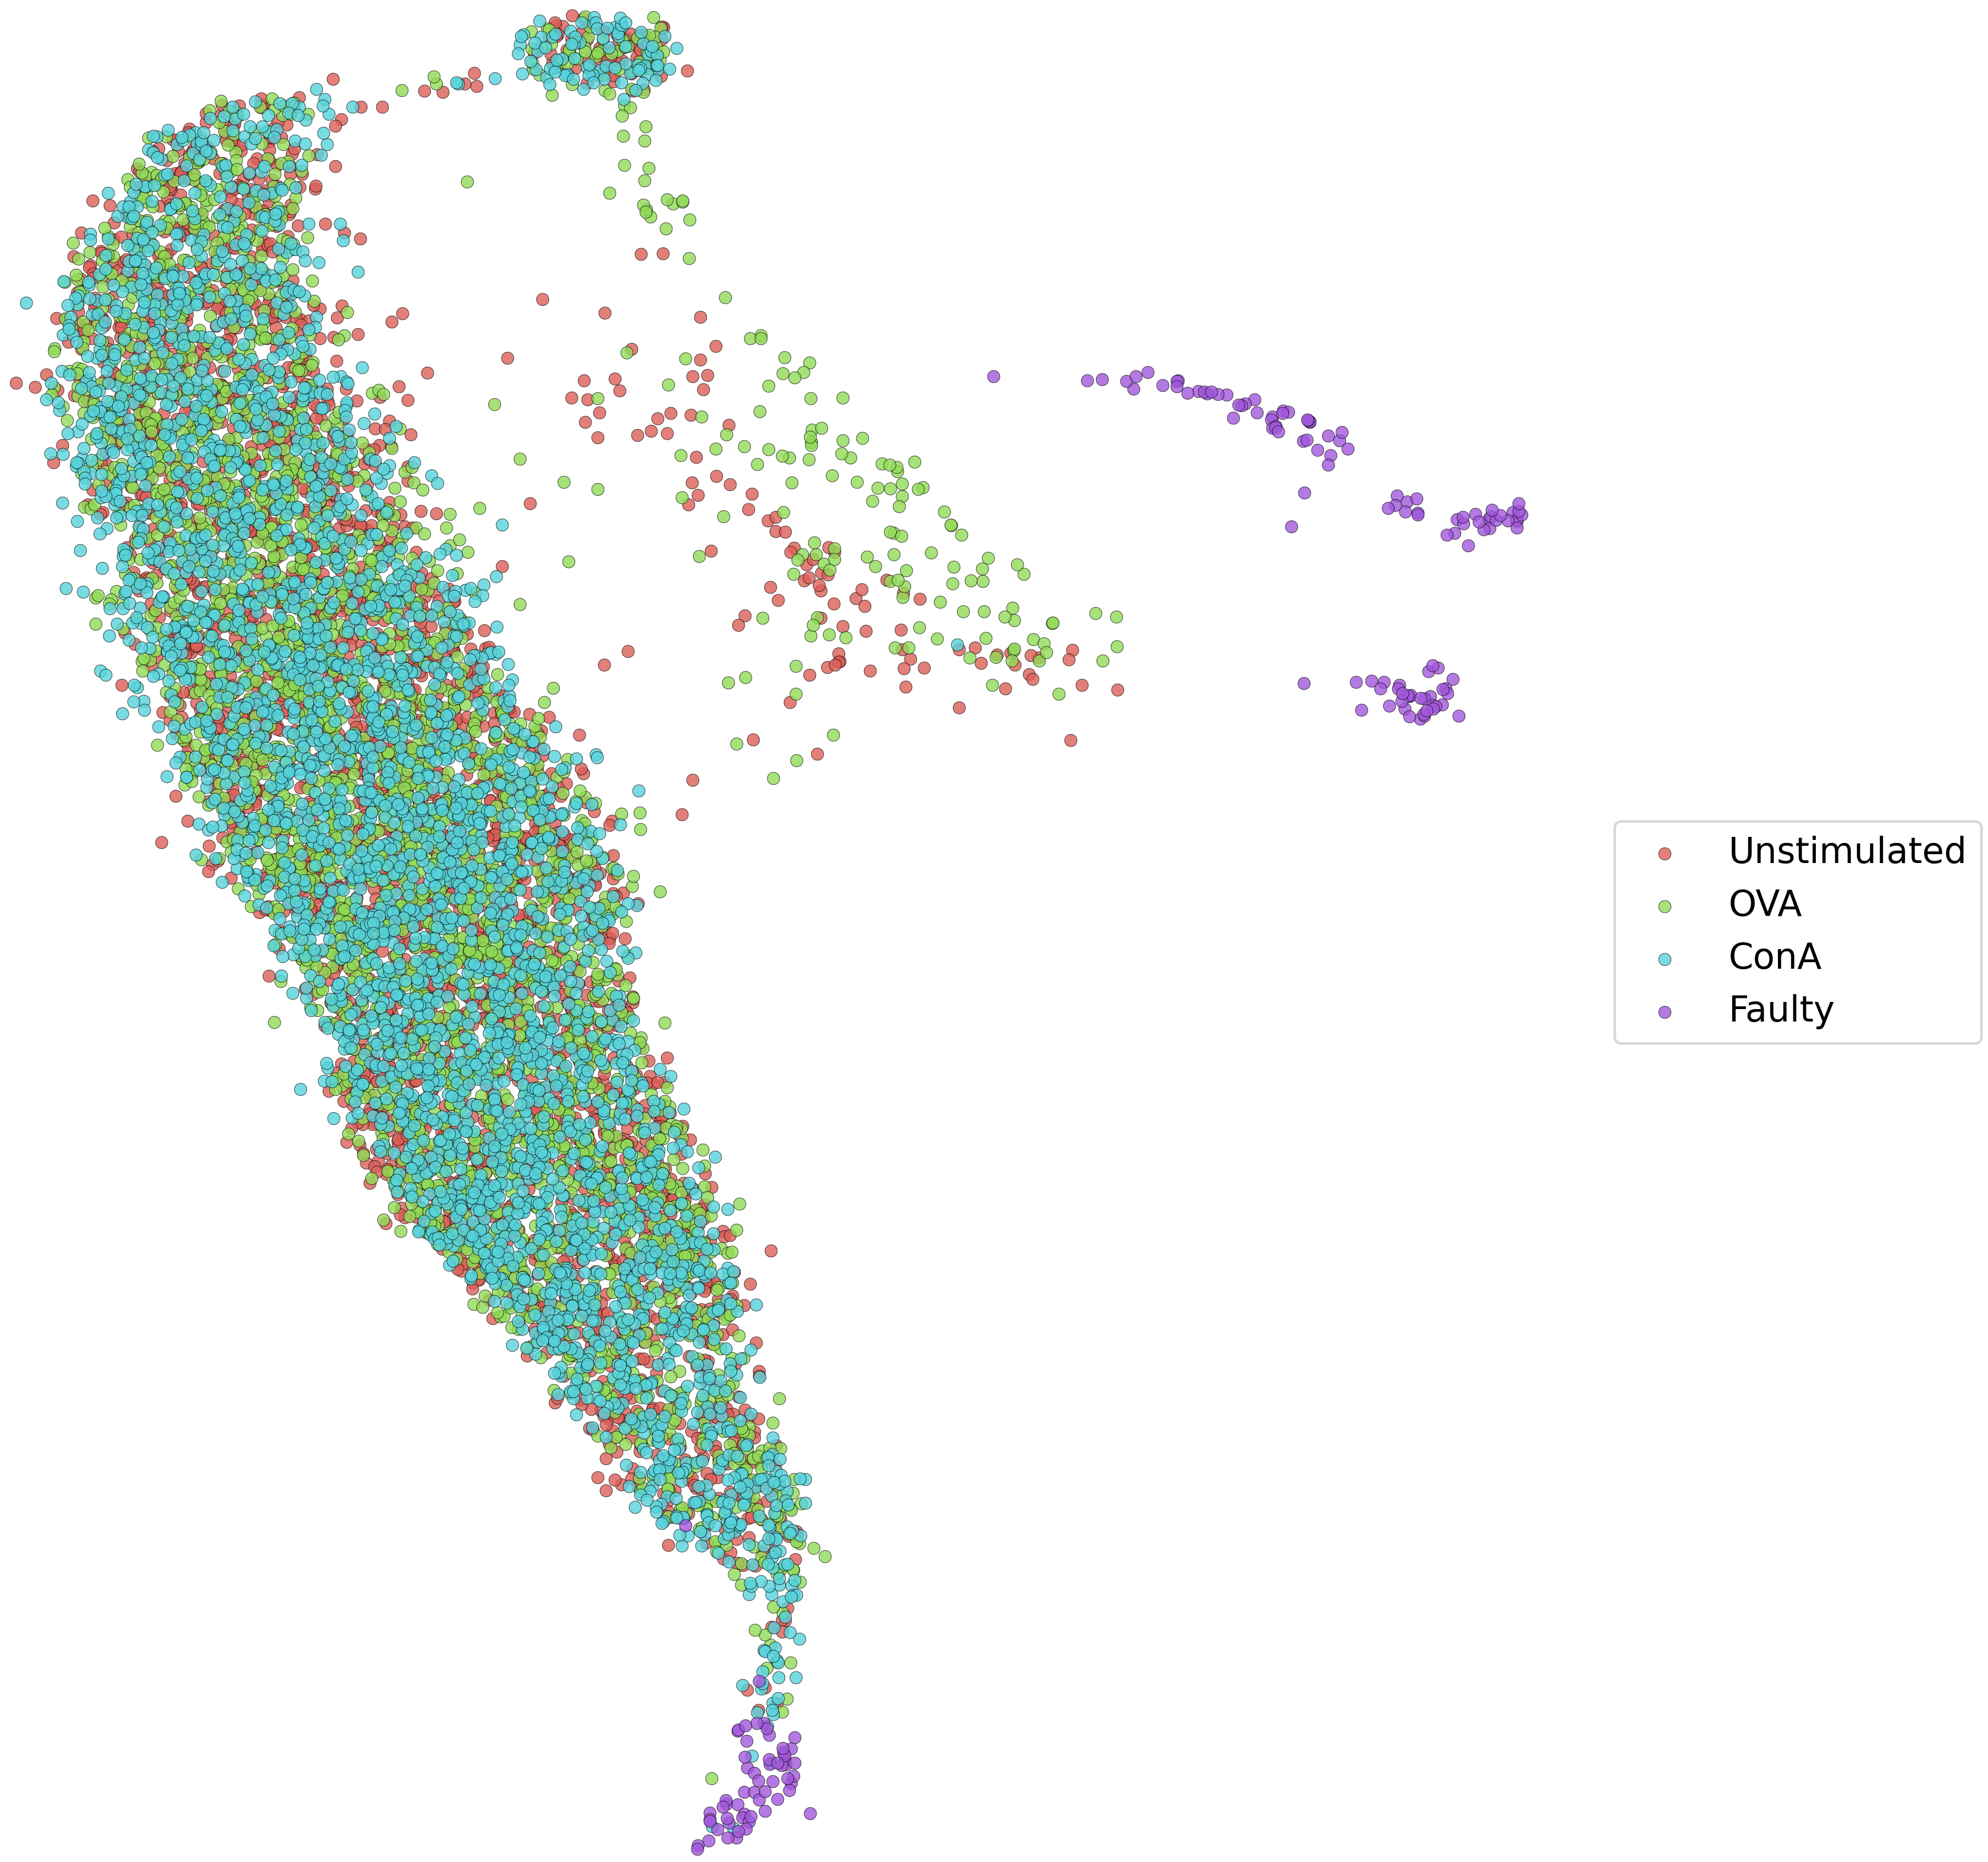
\includegraphics[width=\textwidth]{dissertation/figures/evaluation/CK19_umap.png}
        \caption{Normal images}
        \label{subfig:full_projection_normal}
    \end{subfigure}
    \begin{subfigure}[h!]{0.41\textwidth}
        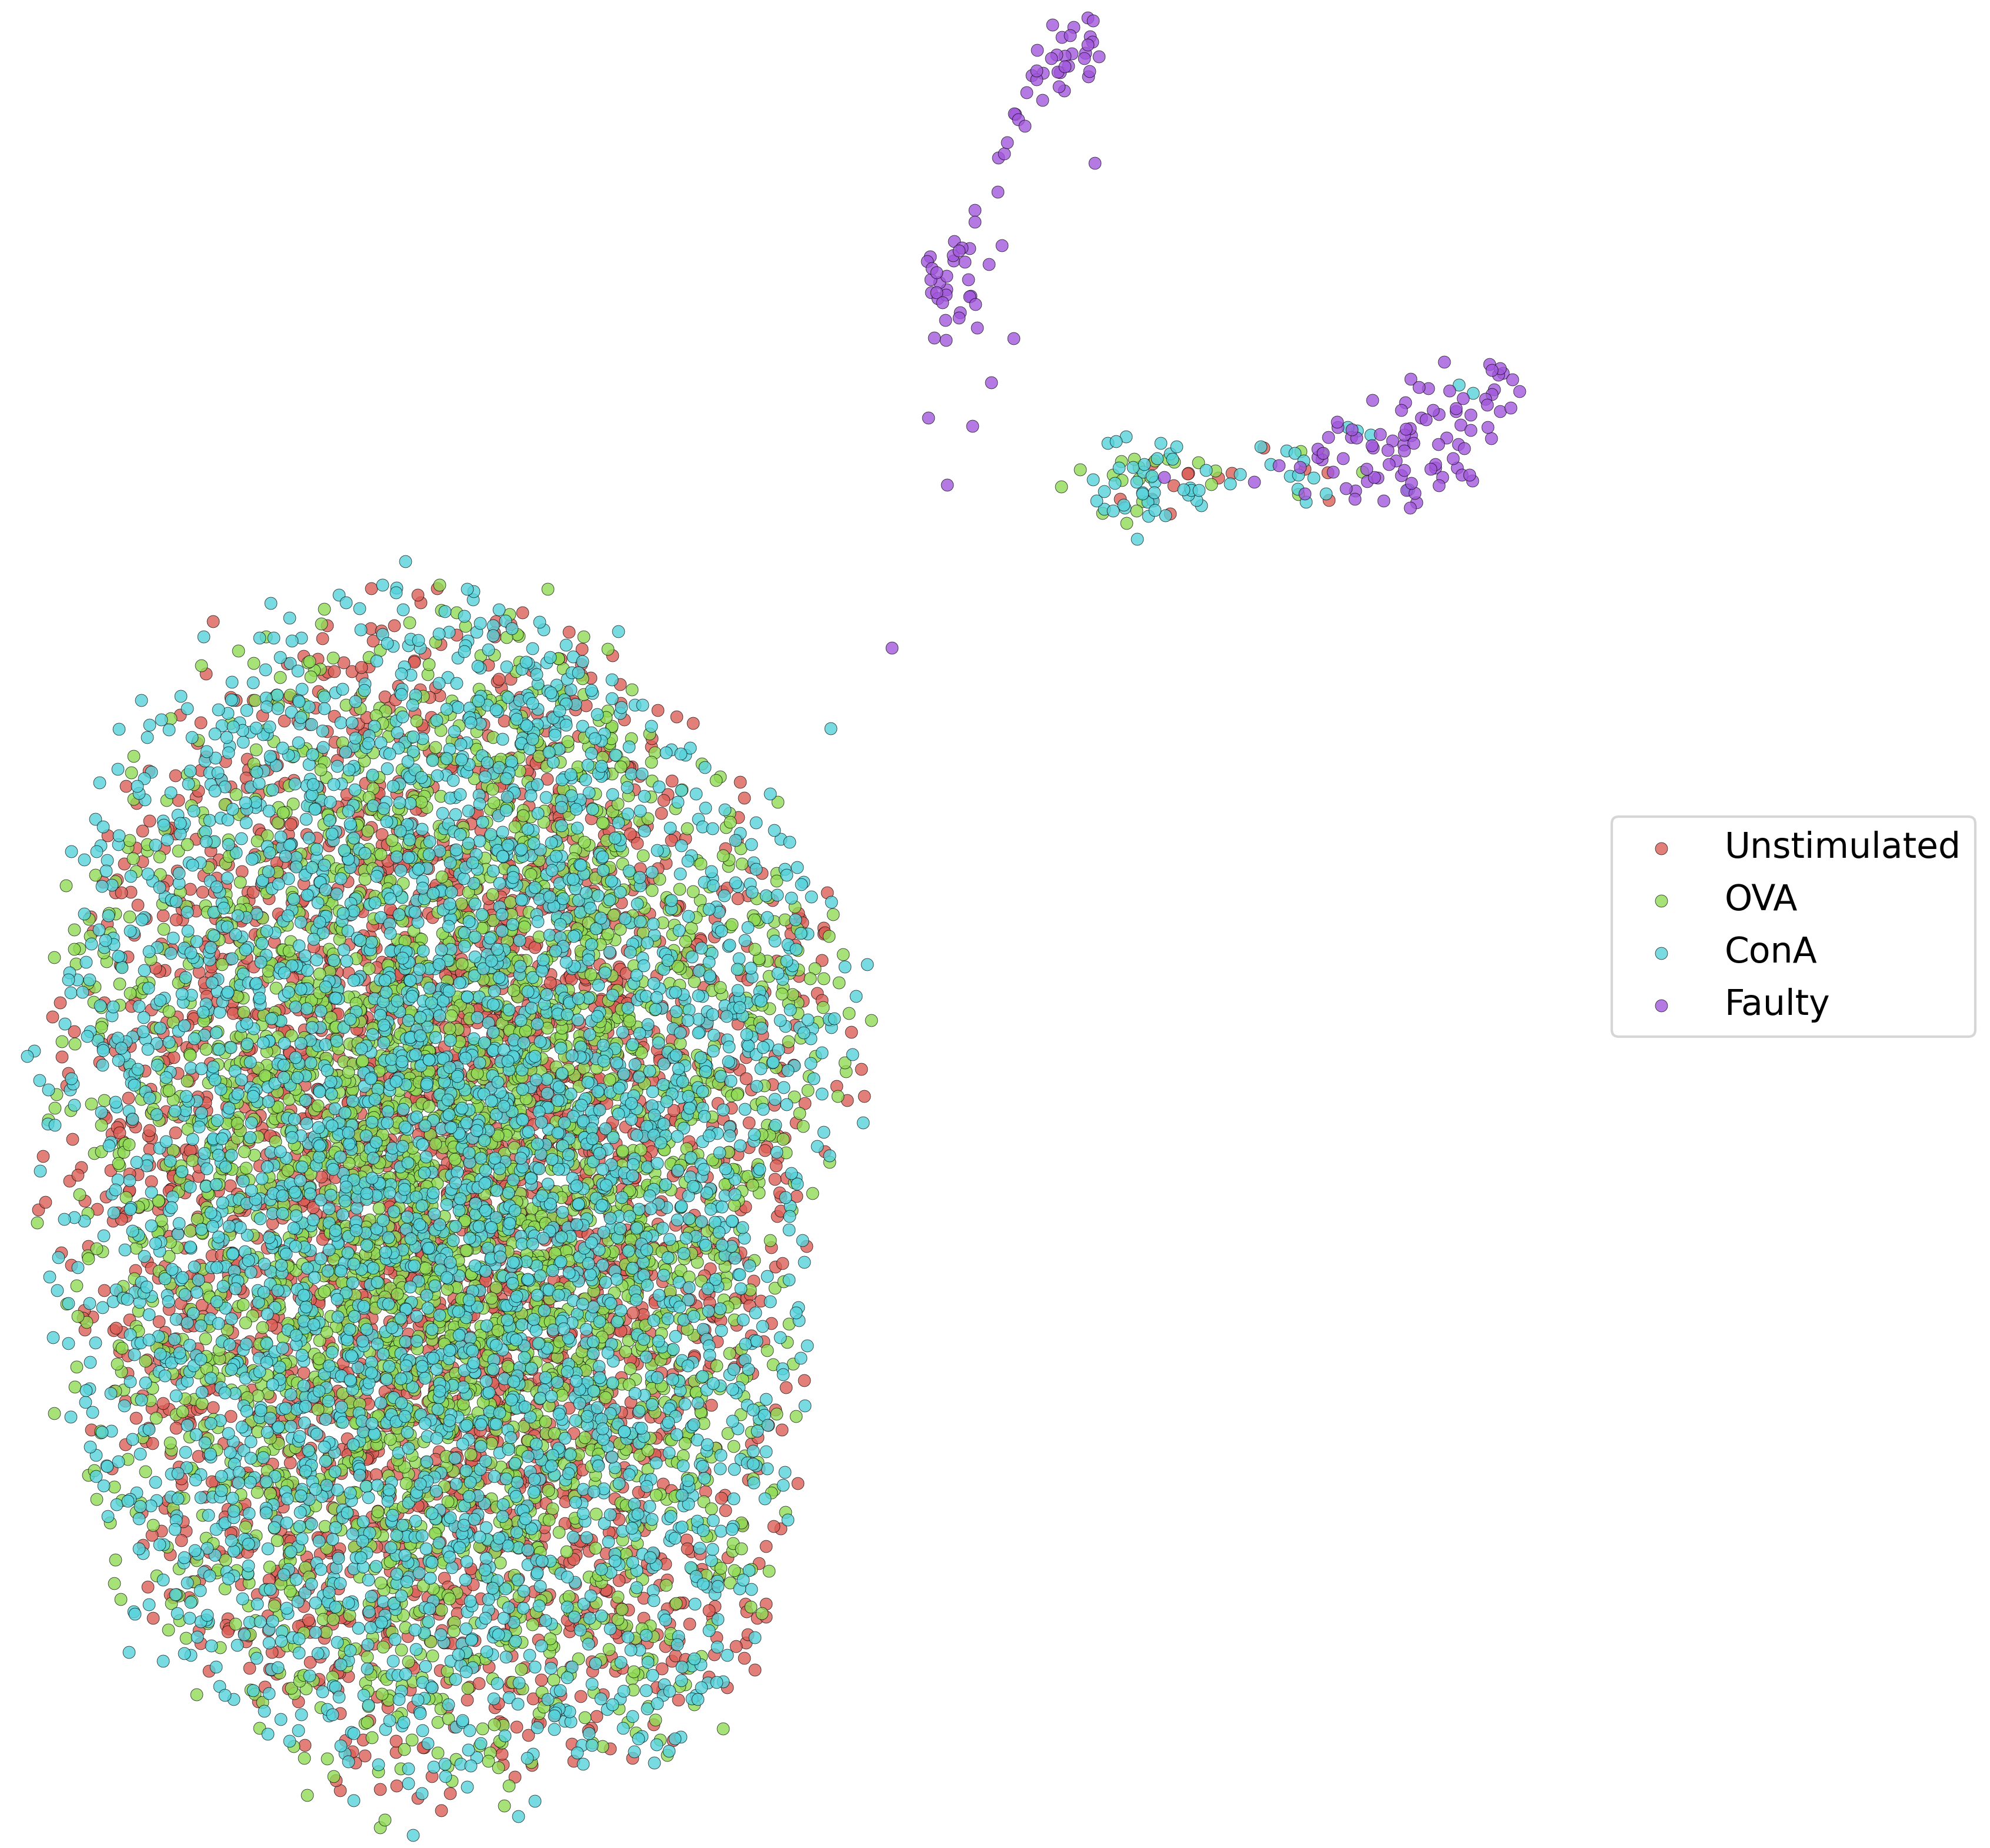
\includegraphics[width=\textwidth]{dissertation/figures/evaluation/CK19_masked_umap.png}
        \caption{Masked images}
    \end{subfigure}
    \caption{Two-dimensional UMAP projections of the 10,000 test images from the \textbf{full} dataset. These projection were obtained with UMAP parameters n\_neighbors=30 and min\_dist=0.8. The legend highlights which colour corresponds to which stimulation category.}
    \label{fig:full_projection}
\end{figure}

We hoped for the \textbf{dual dataset} to perform better as it only had two stimulation categories to distinguish between. The normal and masked visualisations are shown in Figure \ref{fig:dual_visualisation}. Although no clear distinction of clusters is shown the normal projection, a small cluster formed in the projection of the masked dataset. However, this cluster contains images of both \textit{Unstimulated} and \textit{OVA} categories. 

\begin{figure}[ht!]
    \centering
    \begin{subfigure}[ht]{0.35\textwidth}
        \includegraphics[width=\textwidth]{dissertation/figures/evaluation/CK22_umap.png}
        \caption{Normal images}
    \end{subfigure}
    \begin{subfigure}[ht]{0.35\textwidth}
        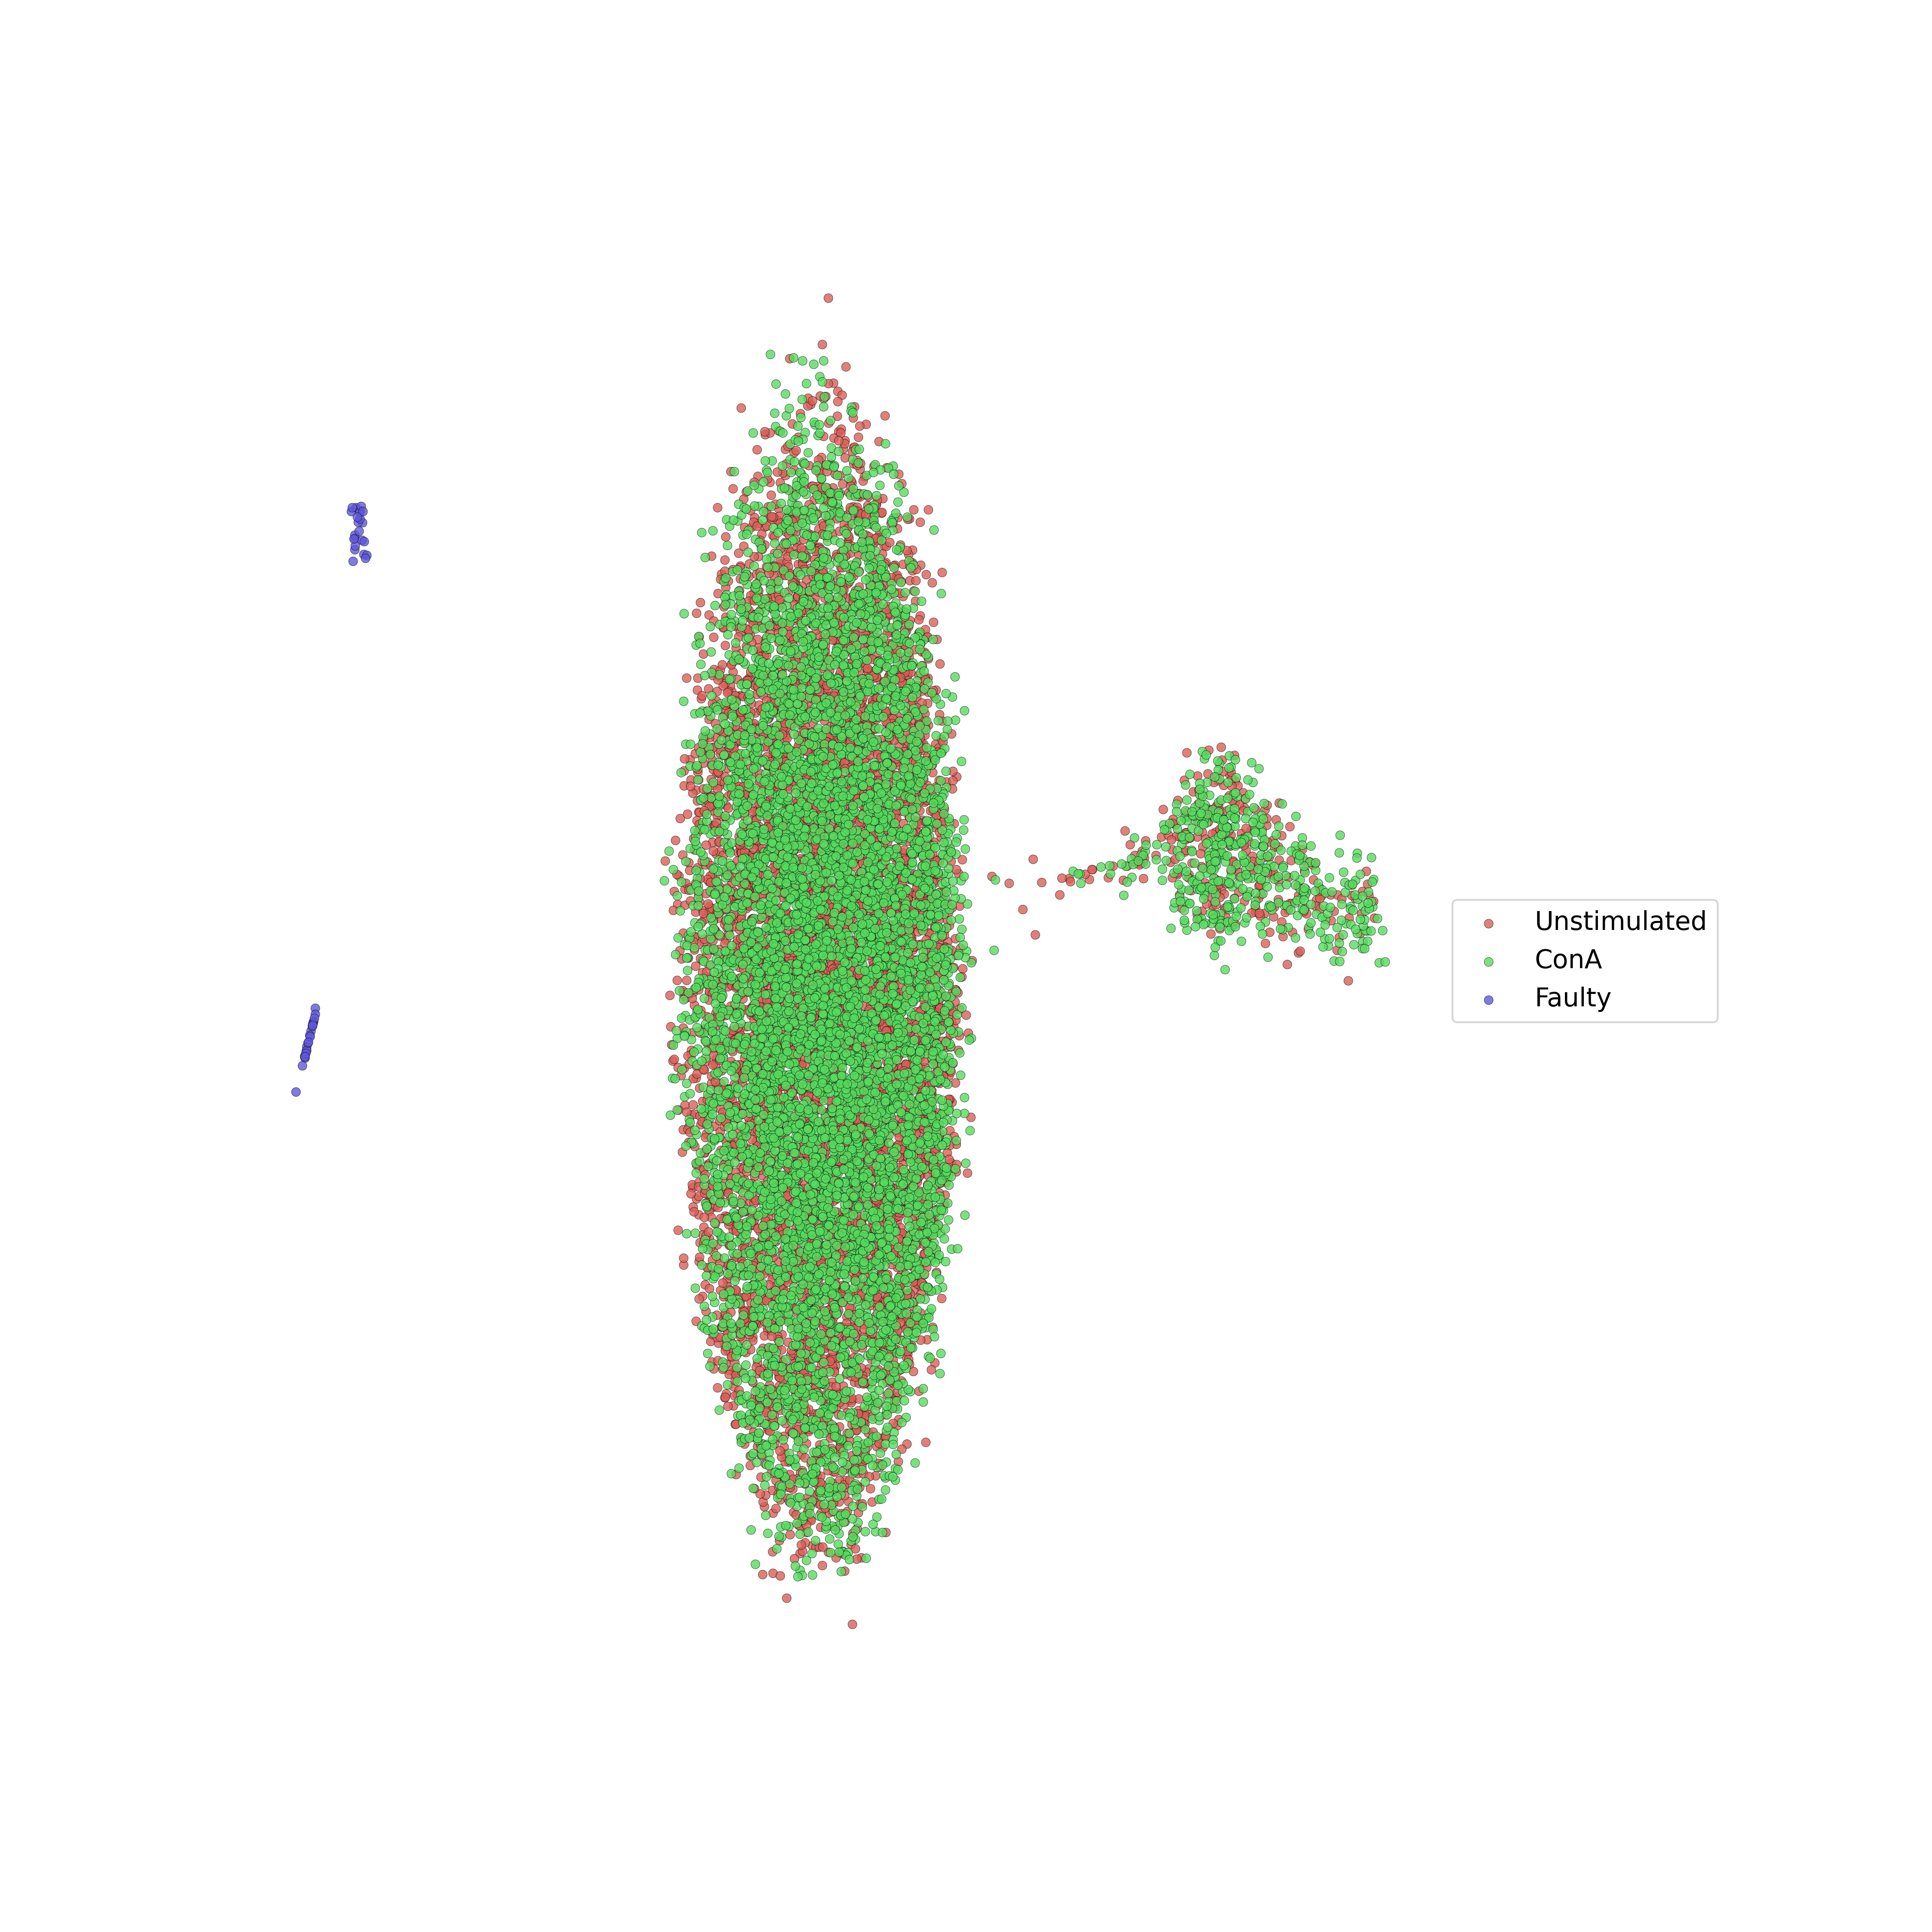
\includegraphics[width=\textwidth]{dissertation/figures/evaluation/CK22_masked_umap.png}
        \caption{Masked images}
        \label{subfig:dual_projection_masked}
    \end{subfigure}
    \caption{Two-dimensional UMAP projection of the 13,800 test images from the \textbf{dual} dataset. These projections were obtained with UMAP parameters n\_neighbors=30 and min\_dist=0.8. The legend highlights which colour corresponds to which stimulation category. The normal images are not clearly distinguished by category, but the masked images yield a separate cluster. None of these clusters bear distinction between images of different stimulation.}
    \label{fig:dual_visualisation}
\end{figure}

The images from the DMSO images should show the most distinction between each other as the immune cells from the images have only been influenced by the stimulation antigens and no other compounds, while immune cells from the experiments represented in the other two datasets have also been injected with drug compounds.

The \textbf{DMSO} projection is shown in Figure \ref{fig:dmso_projection}, from which we can observe some interesting features. Firstly, there is one main cluster, but interestingly the coloured points show a green to blue gradient, which we could attribute to a distinction between the \textit{OVA} and \textit{ConA} categories. Blue/\textit{ConA} points become sparser at the top of the cluster, and the same happens for green/\textit{OVA} points at the bottom of the cluster. This is overlaid on top of images of the \textit{Unstimulated} category, however this might show that some distinction is being made between the images. Furthermore, we can see two smaller collections of red/\textit{Unstimulated} points and green/\textit{OVA} points. The projection of masked images does not show this \textit{OVA-ConA} distinction, but does have a separate cluster of \textit{Unstimulated/OVA} points.

\begin{figure}[h!]
    \centering
    \begin{subfigure}[h!]{0.4\textwidth}
        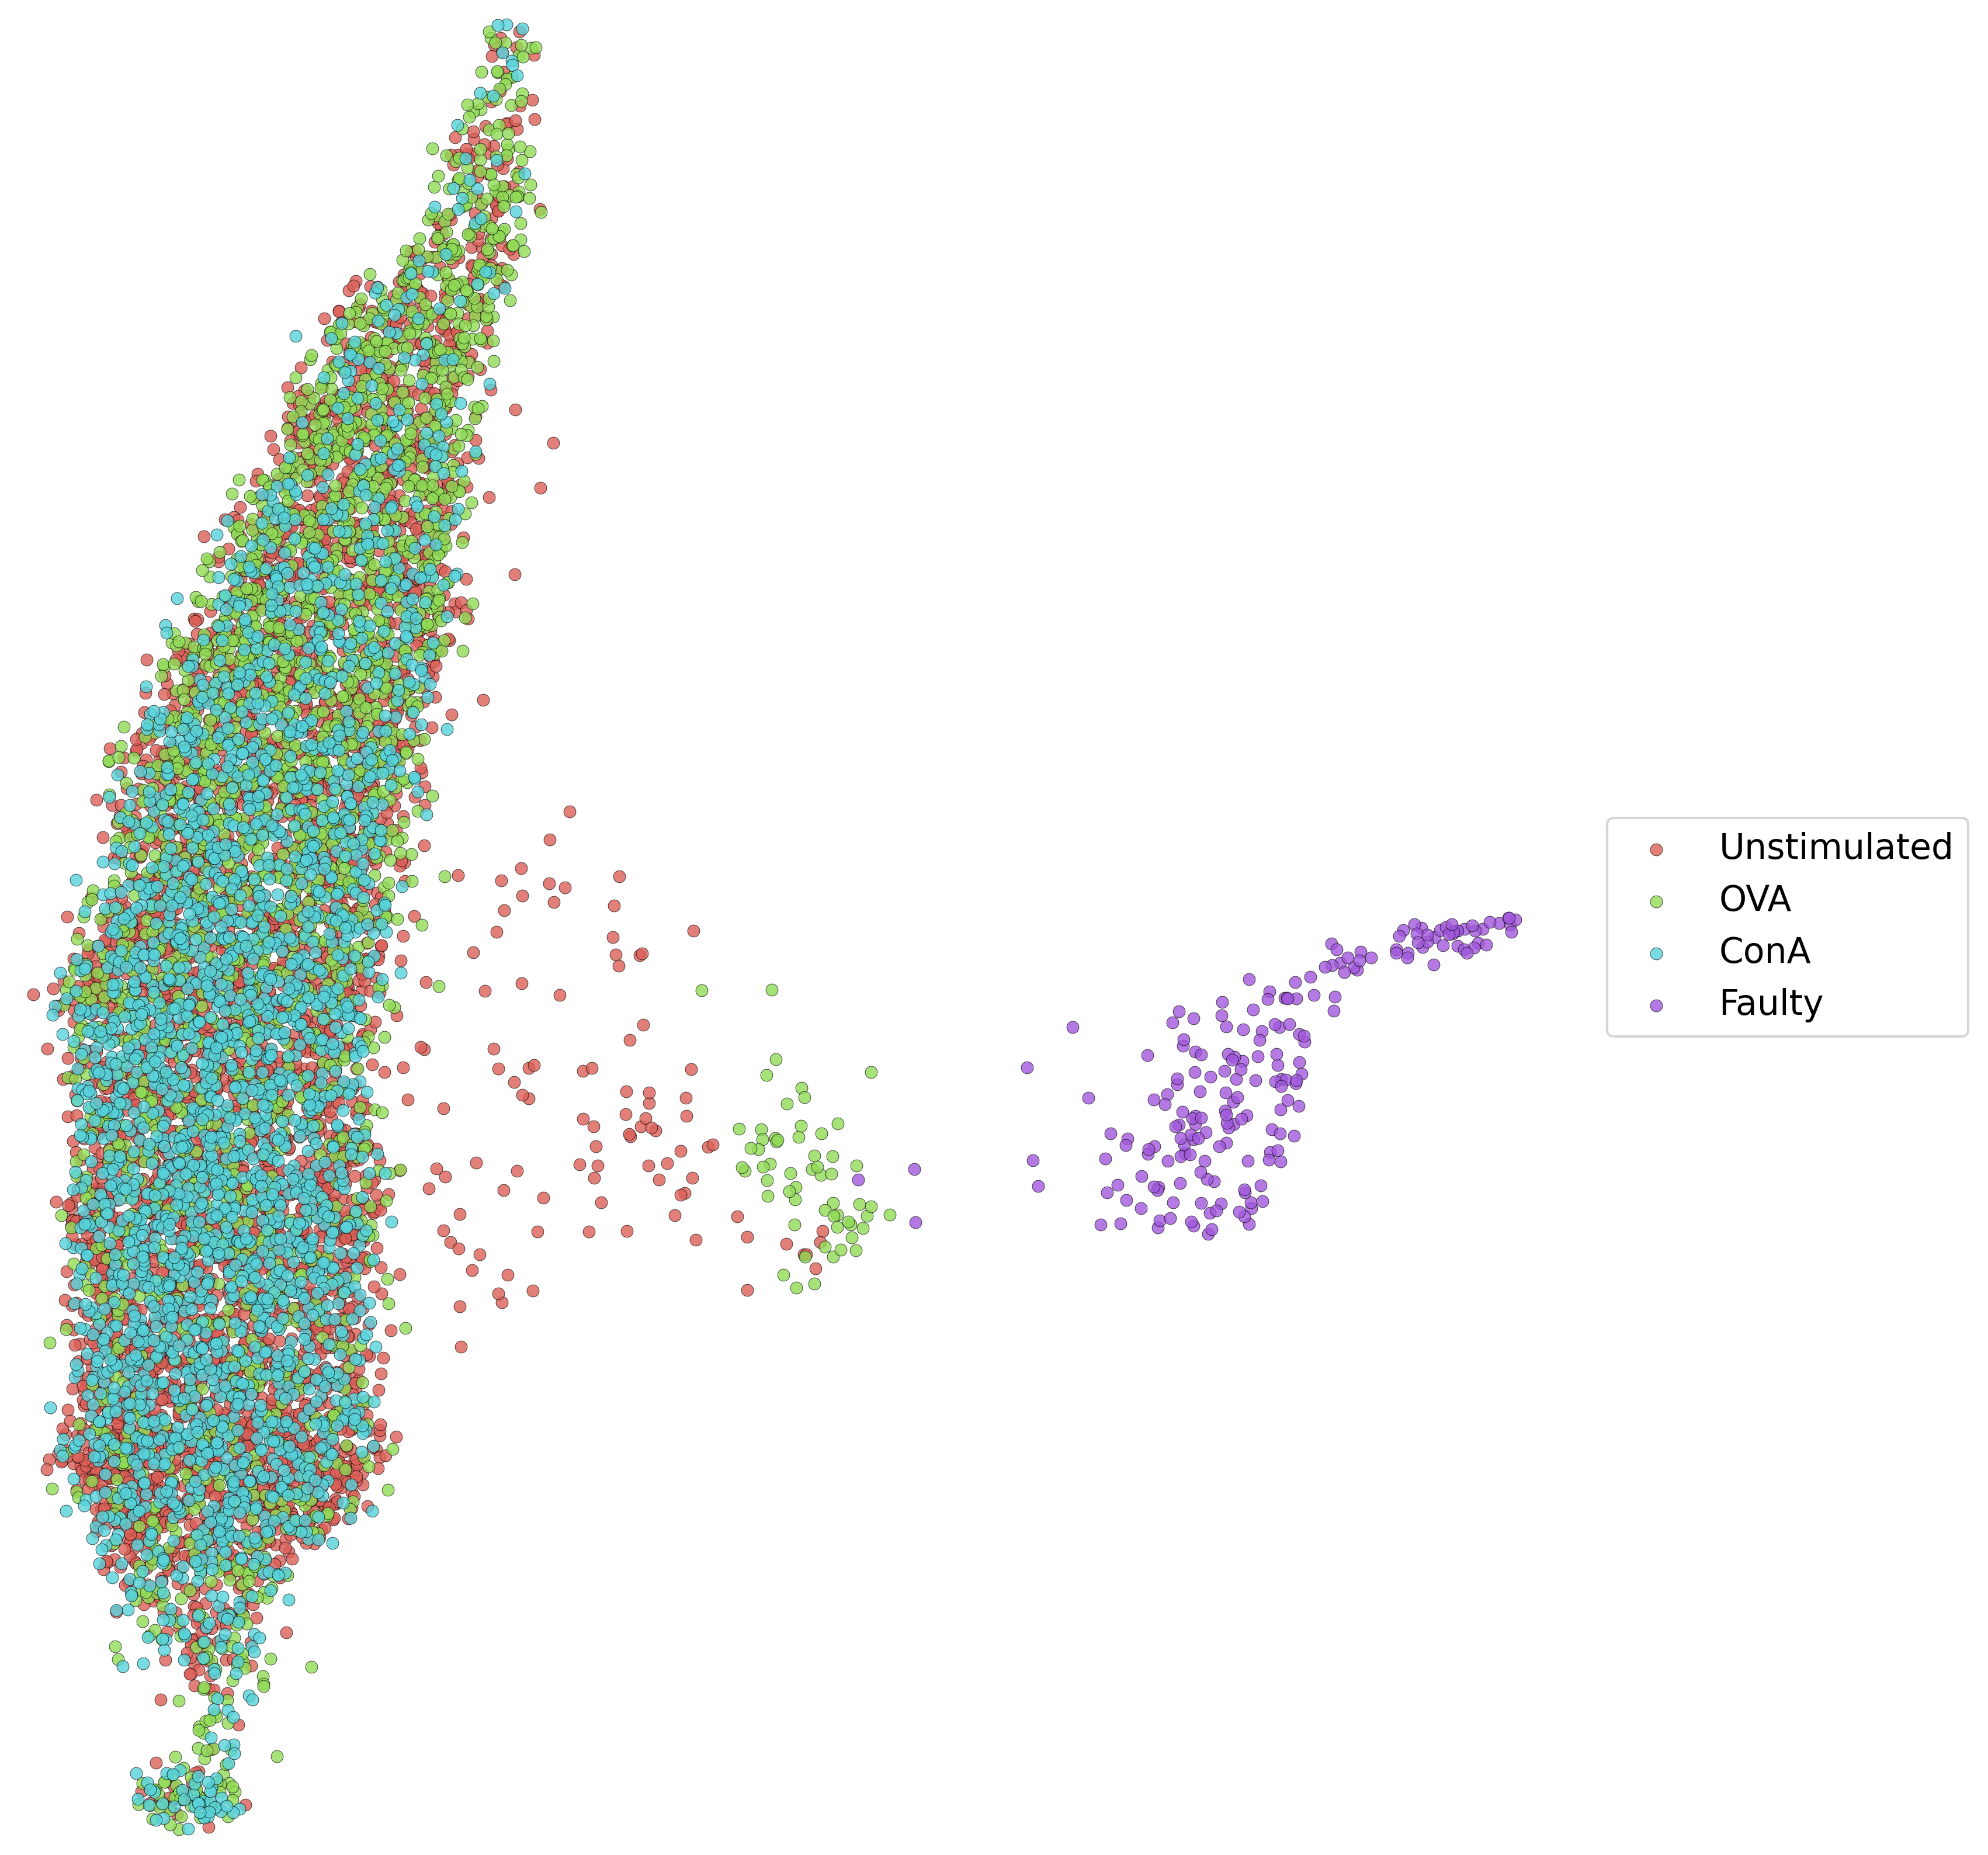
\includegraphics[width=\textwidth]{dissertation/figures/evaluation/DMSO_umap.png}
        \caption{Normal images}
    \end{subfigure}
    \begin{subfigure}[h!]{0.4\textwidth}
        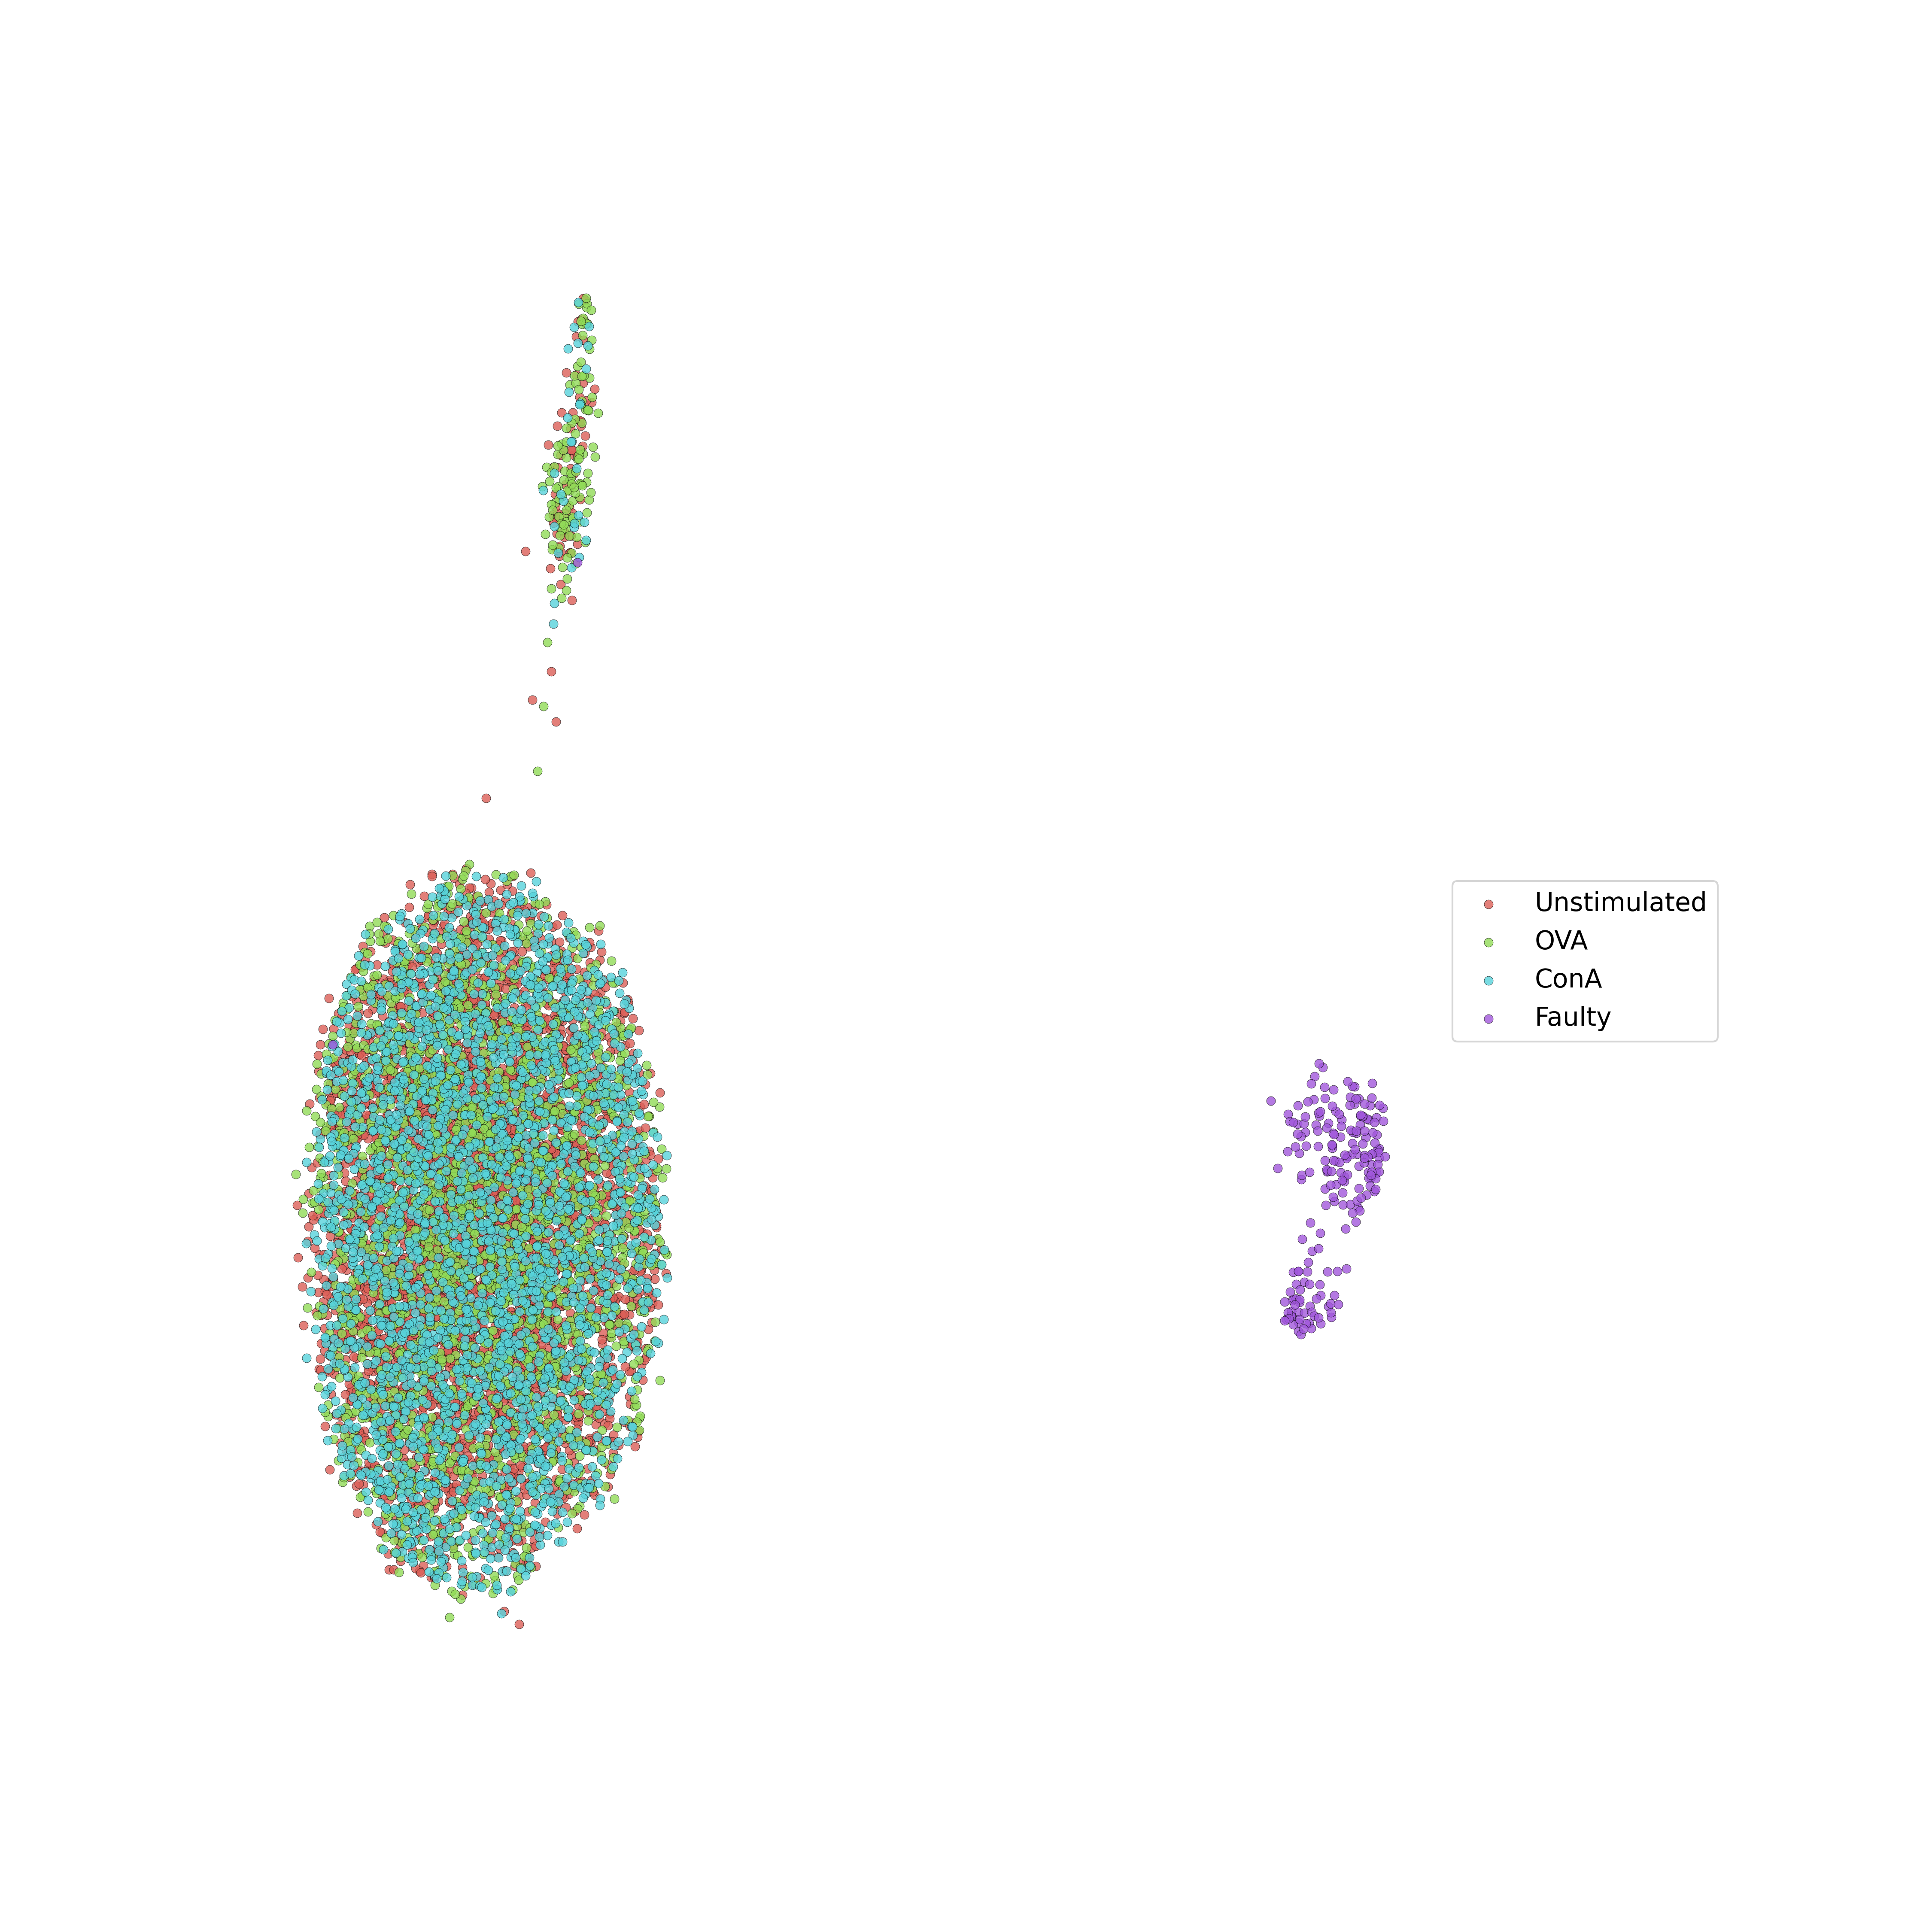
\includegraphics[width=\textwidth]{dissertation/figures/evaluation/DMSO_masked_umap.png}
        \caption{Masked images}
    \end{subfigure}
    \caption{Two-dimensional UMAP projections of the 8,000 test images from the \textbf{DMSO} dataset, which have been noise-corrected (left) and background-corrected (right). UMAP was ran with parameters $n\_neighbors=30$ and $min\_dist=0.8$. The legend highlights which colour corresponds to which stimulation category. In the normal images, the main cluster of points does not show a clear delimitation between images of the same category, however there does seem to be some distinction as we can see a gradient.}
    \label{fig:dmso_projection}
\end{figure}

Every projection highlights that UMAP does not struggle to distinguish \textit{Faulty} images from images containing immune cells. This is useful as it acts as a control that tells us that UMAP is noticing differences in images, and that the autoencoder does not corrupt the images and remove important features. Nonetheless, UMAP did not yield clusters showing any kind of distinction between categories in the cases of the \textbf{full} and \textbf{dual} datasets. A difference is more noticeable in the \textbf{DMSO} dataset. This difference is no longer visible in the masked projection. %This allows us to hypothesise that the experimental conditions used for generating the full and dual datasets do not yield immune cells under different stimulation levels are not structurally different enough in the format they are currently inputted in the dataset, i.e. in small patches of images of size $192\times192\times3$.

\subsection{Are images within the same cluster structurally the same?}

Some projections shown above still showed some clusters and outlier points. We wanted to assess whether the images in these points were indeed structurally similar. In order to explore this, we developed a tool that makes use of matplotlib's animation API\footnote{https://matplotlib.org/api/animation\_api.html}. We can hover over the points of the visualisation to display the original image that is represented by one of the projection points. The drawback of the tool is that it struggles over large clusters of points as it requires quite a lot of memory to update the coordinates in the graph, resize a $192\times192\times3$ image, and display it, and is slow in such cases. 

\begin{figure}[h]
    \centering
    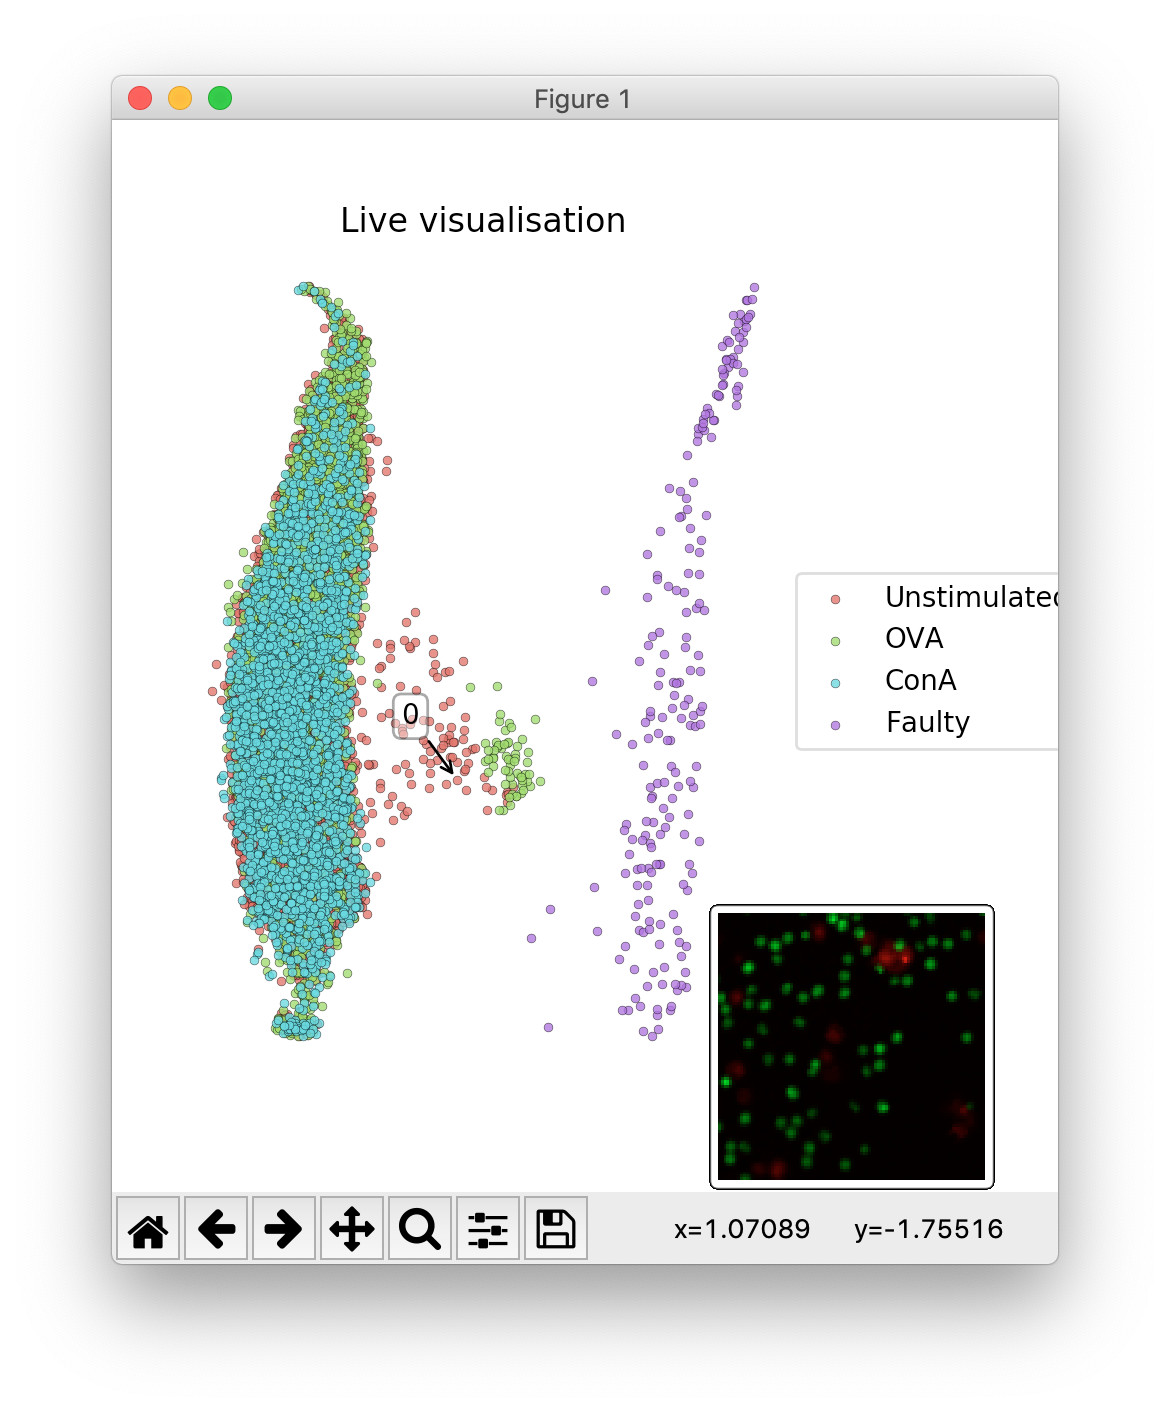
\includegraphics[width=0.32\textwidth]{dissertation/figures/evaluation/right_cluster_big.png}
    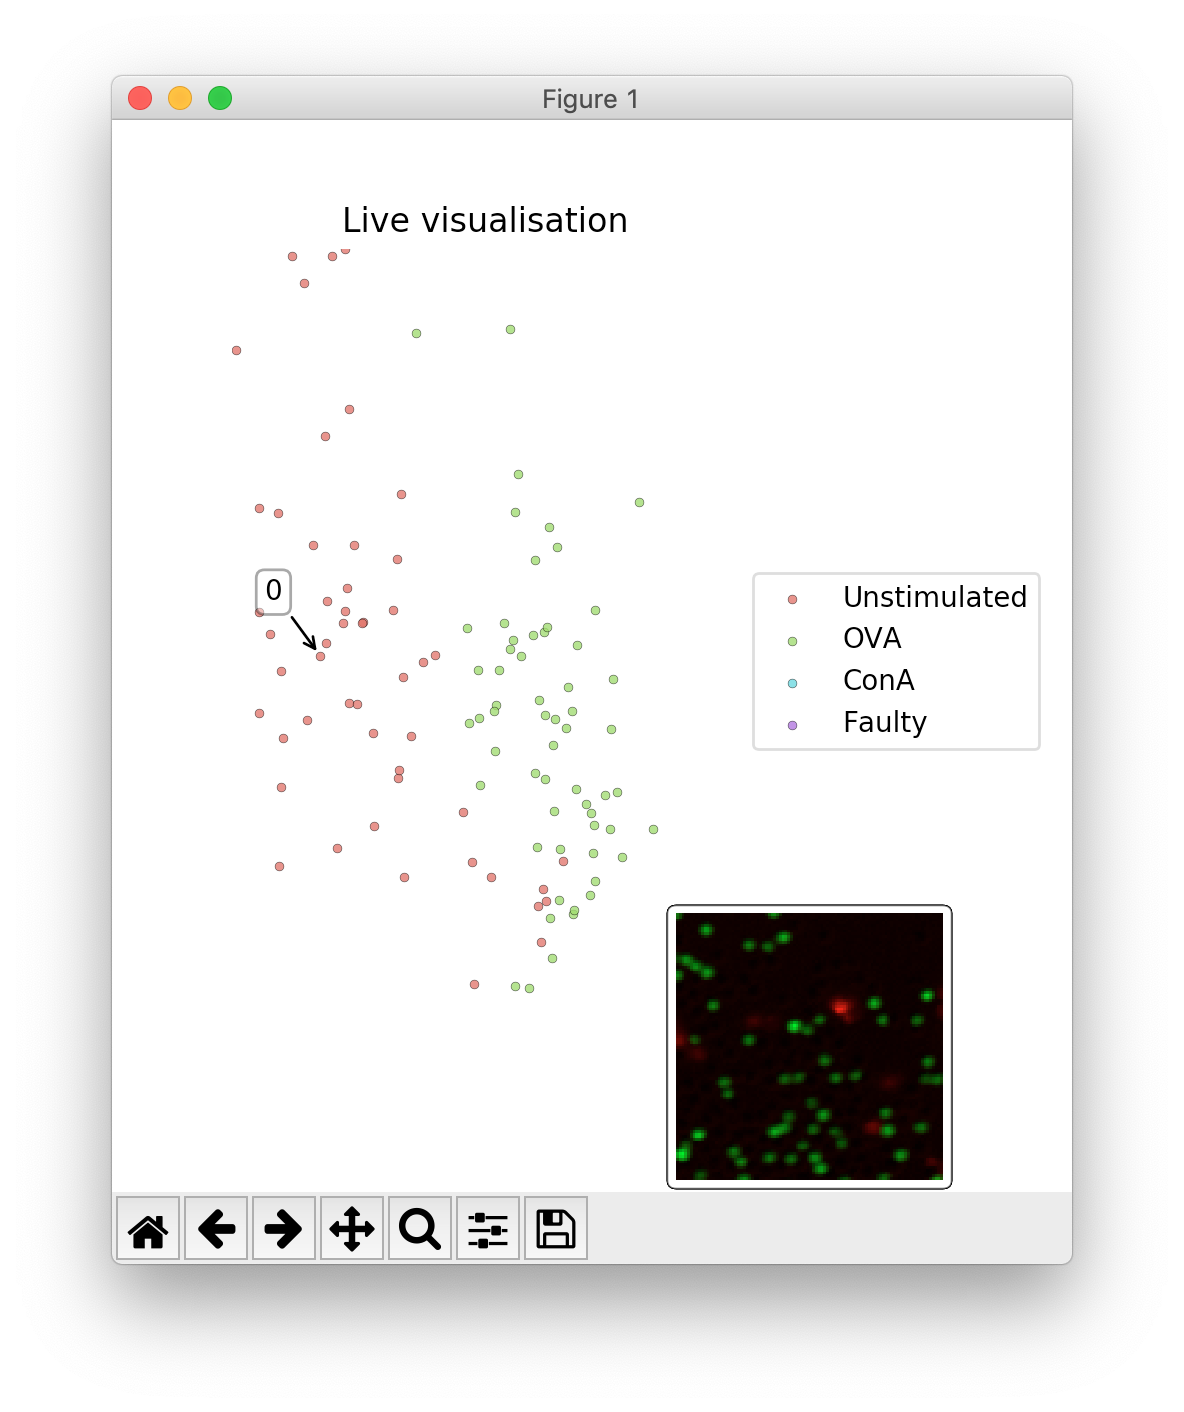
\includegraphics[width=0.32\textwidth]{dissertation/figures/evaluation/right_cluster_red_1.png}
    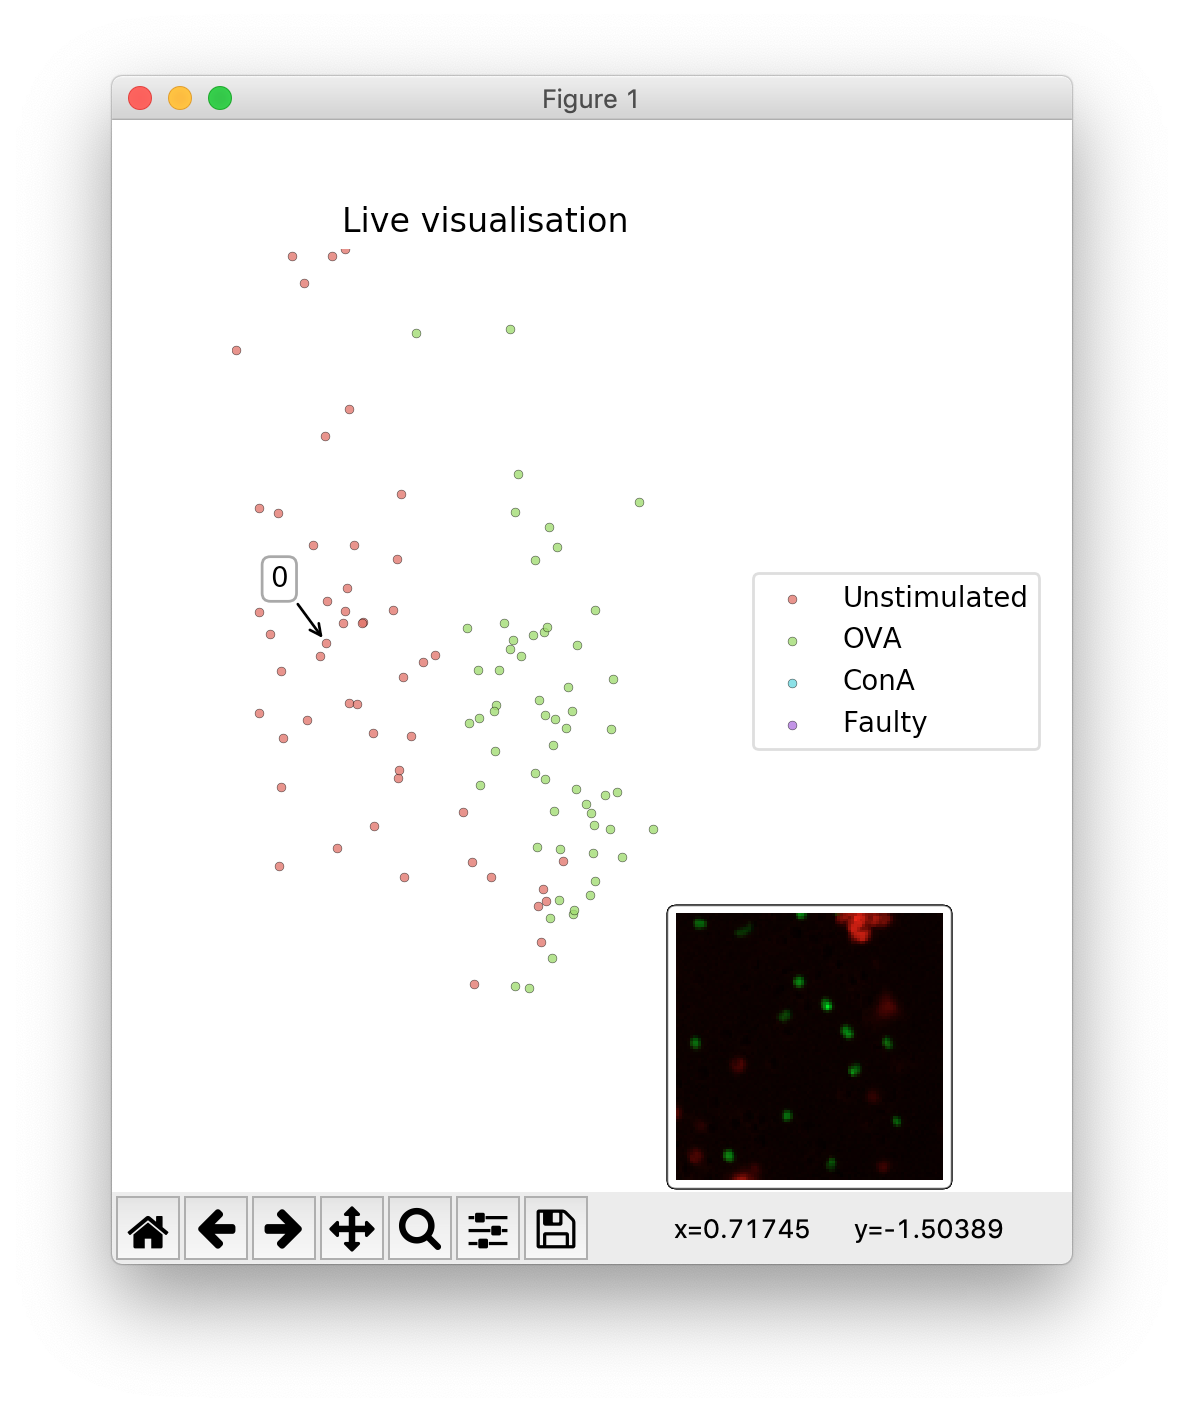
\includegraphics[width=0.32\textwidth]{dissertation/figures/evaluation/right_cluster_red_2.png}
    \caption{Three images extracted from a live visualisation graph of the UMAP projection shown in Figure \ref{fig:dmso_projection}. The graph on the left is unzoomed. The other two graphs have been zoomed in, showing the tool's functionality as well as a closer view of the cluster. We give two example images in the same cluster of similar structure, but one that does not follow the trend.}
    \label{fig:vis_outliers}
\end{figure}

\autoref{fig:vis_outliers} highlight the tool's functionality. We picked the projection of the DMSO dataset from \autoref{fig:dmso_projection} above that showed distinct clusters of images within the same category to evaluate whether or not they were meaningful. The projection in the first image will look slightly different as the plot is of smaller size and the method for drawing the scatter plots had to be adapted for the task. We then zoom over clusters of interest to be able to pick out points more efficiently. This view shows us that we can find two images within the same cluster that look structurally the same, but another image which does not is also in that same structure. 

\autoref{fig:vis_outliers_2} shows a different case. We highlight three points in a cluster which are close to each other and show they are similar – they all are a particular hue of green. This highlights that our noise correction was not necessarily successful in all cases, and explains why less clusters are found with the masked images. 

\begin{figure}[h]
    \centering
    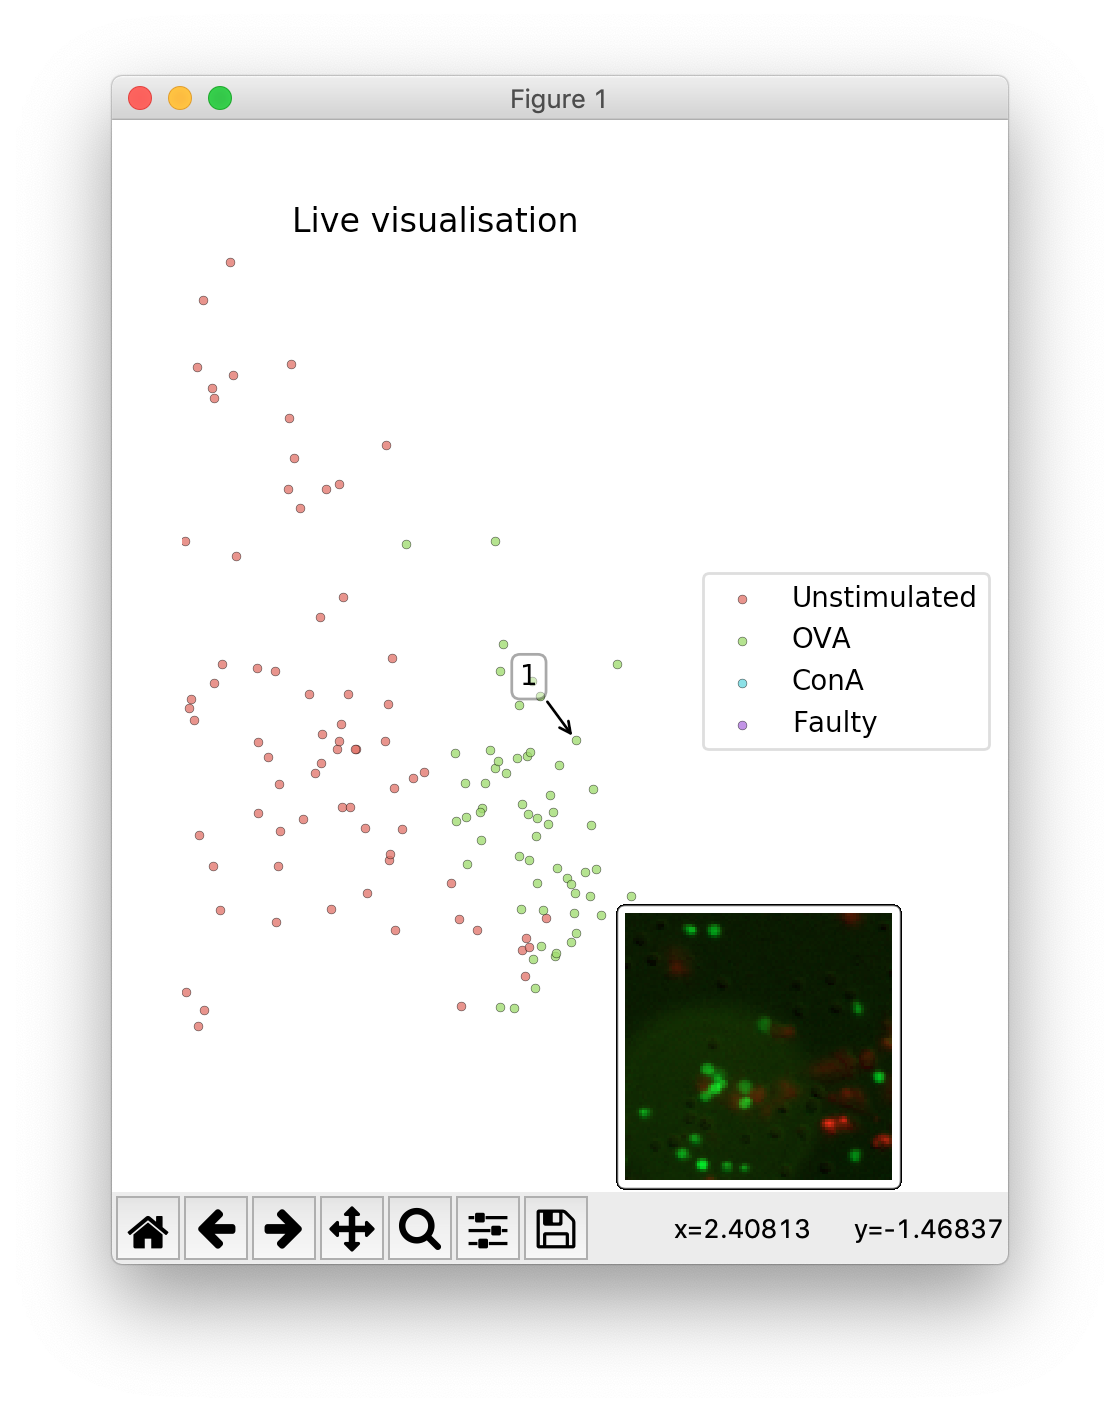
\includegraphics[width=0.32\textwidth]{dissertation/figures/evaluation/green_cluster_1.png}
    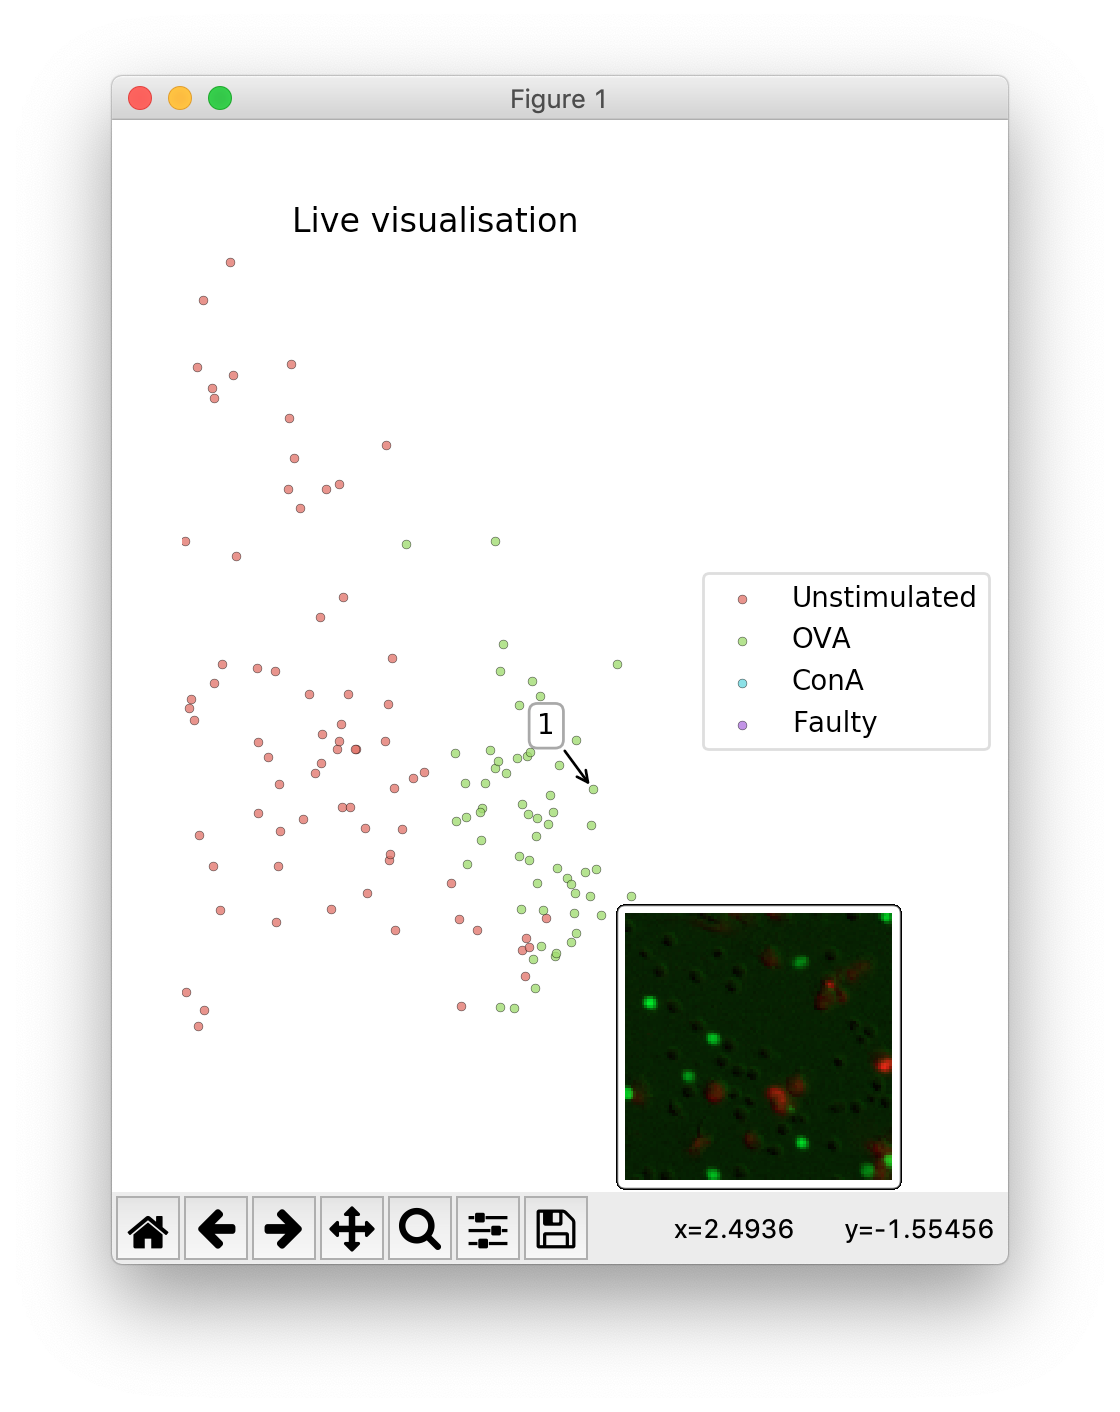
\includegraphics[width=0.32\textwidth]{dissertation/figures/evaluation/green_cluster_2.png}
    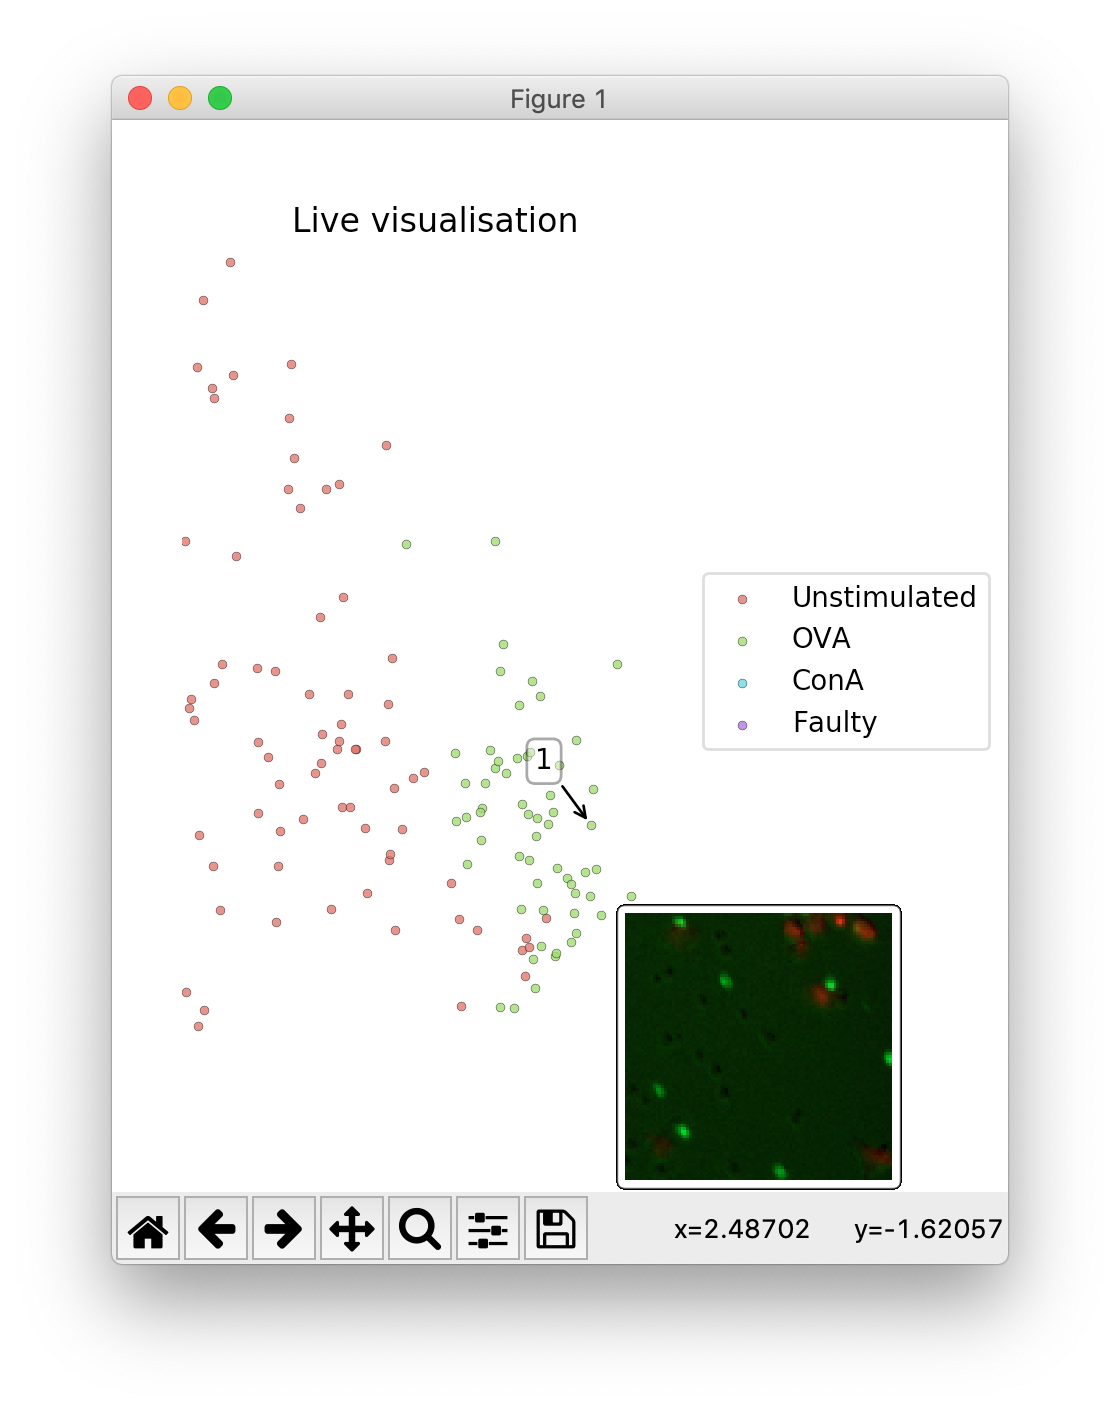
\includegraphics[width=0.32\textwidth]{dissertation/figures/evaluation/green_cluster_3.png}
    \caption{Three images extracted from a live visualisation graph of the UMAP projection shown in \autoref{fig:dmso_projection}. The graph has been zoomed in to the distinctive green cluster. This highlights three images that are similar – they are all a shade of green.}
    \label{fig:vis_outliers_2}
\end{figure}

\subsection{Are our visualisations more meaningful with interaction measure meta-data?}

In the case of visualisations that did yield some groupings, but contained points of mixed categories, we hypothesised that other meta-data about the images might explain why some clusters were formed. Indeed, maybe the stimulation level of immune cells was not creating enough distinction between images, and they were more influenced by something else. For example, how much the cells overlapped in the image, regardless of their stimulation category. 

We plotted the visualisations again, but using the interaction measures collected with the intersection-over-union metric to change the size of the markers. We decided to tweak the visualisations shown in Figure \ref{subfig:full_projection_normal} and Figure \ref{subfig:dual_projection_masked} as they yielded some separated groupings, but of mixed labels. The results are shown in \autoref{fig:size_visualisation} below. 

\begin{figure}[h!]
    \centering
    \begin{subfigure}{.45\textwidth}
        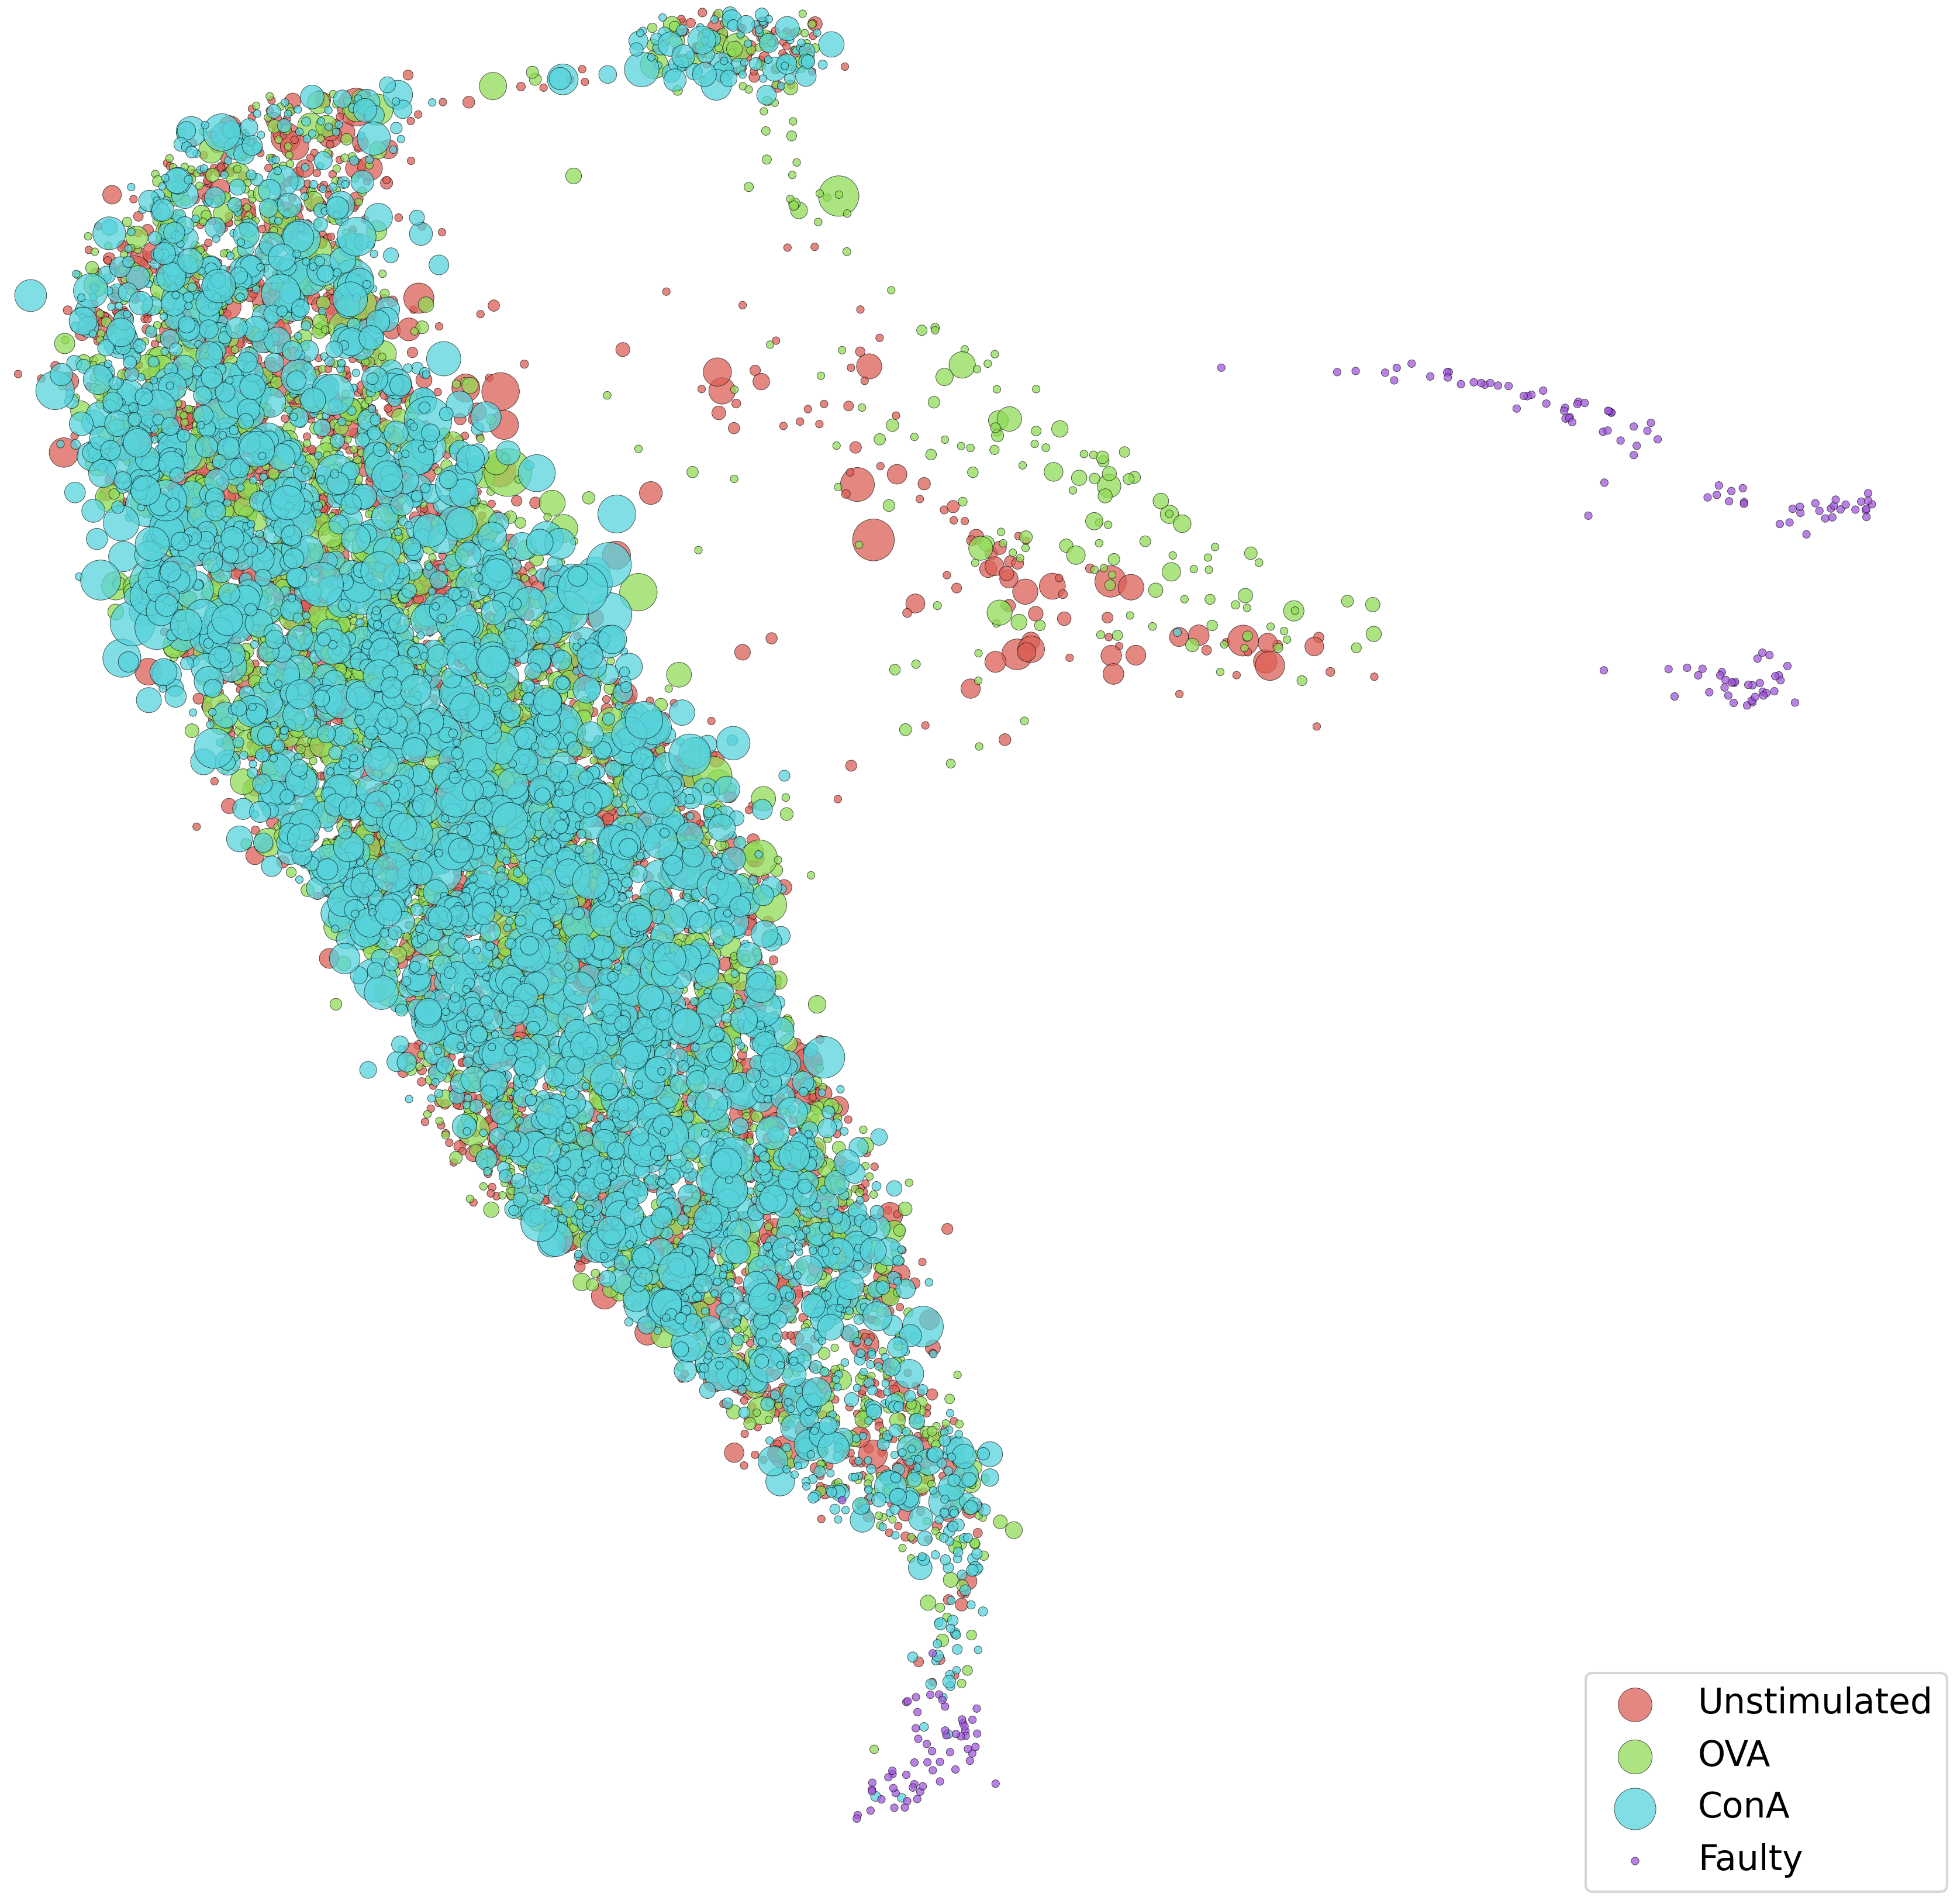
\includegraphics[width=\textwidth]{dissertation/figures/evaluation/CK19_umap_size.png}
        \caption{UMAP projection of the full dataset}
    \end{subfigure}
    \begin{subfigure}{.45\textwidth}
        \includegraphics[width=\textwidth]{dissertation/figures/evaluation/CK22_masked_umap_size.png}
        \caption{UMAP projection of the masked dual dataset}
    \end{subfigure}
    \caption{UMAP projections for the full dataset and masked dual dataset, tweaked with the size of overlap in each image as the size of the scatter points. The legend shows the category of each point as well as the average size of the points.}
    \label{fig:size_visualisation}
\end{figure}

These visualisations show us that although all images in the separated clusters contain a similar level of interaction, some other images in the main clusters also have that level of interaction. As such, we also cannot say that UMAP is finding structure in the images based on how much overlap (i.e. shades of orange) there is.

\section{Regression}

Our regression task is to predict the percentage of overlap between T-cells and dendritic cells from an image where T-cells are shaded green, and dendritic cells are shaded red.

\subsection{Metrics}

Our regression model is trained on mean squared error (MSE). We decided to evaluate on root-mean-square-error (RMSE) as it is a common metric for evaluating the difference between predictions of a model and actual truth values: RMSE has the advantage of being in the same unit as the dependent variable. In our case the unit is the percentage of overlap between the cells objects obtained with intersection-over-union. RMSE is defined as the square root of the quadratic mean of the difference between our predicted values and their truth values. The equation is as follows:

\begin{equation}
    RMSE = \sqrt{\frac{1}{n}{\Sigma_{i=1}^{n}{\Big({\hat{y}_i-y_i})}^2}}
\end{equation}

where $n$ is the number of samples in the dataset, $y$ is the true value of a sample, and $\hat{y}$ is the predicted value of a sample. 

We also include the (unbiased) standard deviation (SD) of our predicted results to express their variability. The formula for SD is as follows:

\begin{equation}
    \sigma = \sqrt{\frac{1}{n-1}\Sigma_{i=1}^{n}{(\hat{y}_i - \mu)}^2}
\end{equation}

where $n$ is the number of predicted samples, $\hat{y}_i$ is the predicted value of a sample and $\mu$ is the mean of all predicted values. 

\subsection{Can we quantify interaction from an image of immune cells?}

We evaluate the predictions made by the normal and masked regression models by looking at the predictions of each dataset in each stimulation category, however the model was not fed any stimulation category labels during training. Nonetheless, we might see more overlap across different stimulation categories if they generate more interaction between immune cells, so it is important to also look at errors in prediction within those ranges of values.

\bigskip
\subsubsection{Full dataset}
\hfill
\hfill 

Our regression model reports an overall score of 1.838 $\pm$ 4.583 on the test instances of the full dataset. The masked regression model trained on the images which have a black background reports a score of 1.161 $\pm$ 4.732, which shows an improvement in RMSE. Variance in the true values is of 4.853 overall, meaning that we can see a very similar amount of variance in the predicted values. Table \ref{tab:full_rmse} reports the full scores on all stimulation categories. 

\begin{table}[h!]
\centering
\caption{Average RMSE and SD scores (in \%) for the regression model's predictions on the \textbf{full} dataset. The closer the value is to 0, the closer the prediction is. We can see that the difference remains quite low across all datasets, with ConA having the highest RMSE and SD.}
\label{tab:full_rmse}
\begin{tabular}{l|rrr|r}
\rowcolor[HTML]{EFEFEF}
\textbf{Images} & \cellcolor[HTML]{FFCCC9}\textbf{Unstimulated} & \cellcolor[HTML]{C9FFCB}\textbf{OVA} & \cellcolor[HTML]{96FFFB}\textbf{ConA} & \textbf{All} \\ \hline
Normal      & 1.344 $\pm$ 3.102  & 1.387 $\pm$ 2.963   & 2.502 $\pm$ 6.004  &   1.838 $\pm$ 4.583  \\ \hline
Masked      &    0.832 $\pm$ 3.174          & 0.766 $\pm$ 3.355  &  1.642 $\pm$ 6.067   &   1.161 $\pm$ 4.732 
\end{tabular}
\end{table}

We can see that the \textit{ConA} category has a higher RMSE score, while \textit{Unstimulated} and \textit{OVA} scores are similar. Given the large standard deviations on each of the scores, the differences between them for each different stimulation category cannot be considered statistically significant. The high standard deviation for images with \textit{ConA} stimulation could be partly explained with the range of values for that category. 

\begin{figure}[h!]
    \centering
    \begin{subfigure}{.8\textwidth}
        \includegraphics[width=\textwidth]{dissertation/figures/evaluation/CK19_scatter.png}
        \caption{Normal images}
    \end{subfigure}
    \begin{subfigure}{.8\textwidth}
        \includegraphics[width=\textwidth]{dissertation/figures/evaluation/CK19_masked_scatter.png}
        \caption{Masked images}
        \label{fig:full_masked_scatter}
    \end{subfigure}
    \caption{Scatter plot comparing true values (x-axis) to predicted values (y-axis) for the \textbf{full} dataset. The line of best fit is the straight continuous line running diagonally true the plot, which is the line we want our predictions on. The predictions are plotted for, from left to right: Unstimulated (red), OVA (green), and ConA (blue). Each sub-plot is not on the same scale as each category does not have the same range of overlap values, but we wanted to show more granularity for each sub-plot.}
    \label{fig:full_scatter}
\end{figure}

Figure \ref{fig:full_scatter} is a scatter plot showing the line of best fit for our predictions. In the ideal scenario, where the regression model always makes the right prediction, each point should be placed on the diagonal line. We can see that that in the \textit{Unstimulated} category, points struggle to follow this line. There is a large number of errors when the value to predict is closer to 0. This is also the case for the \textit{OVA} and \textit{ConA} categories, although less so. Furthermore, the plot shows that images in the \textit{ConA} category have a higher percentage of overlap in general. This could explain why the \textit{ConA} category yields a higher RMSE and SD score. In fact, if more points in the \textit{Unstimulated} and \textit{OVA} categories have an overlap value of 0, then it would explain why they have a smaller RMSE and SD score. 

\begin{figure}[h!]
    \centering
    \includegraphics[width=.8\textwidth]{dissertation/figures/evaluation/CK19_histogram.png}
    \caption{Histogram showing the distribution of overlap values for each stimulation category. The true values are at the bottom, and the predicted values for the normal dataset are at the top. Most images have an overlap value of around 0, and images in the ConA category show the biggest overlaps.}
    \label{fig:full_histogram}
\end{figure}

To illustrate this, we show the distribution of the true and predicted values of overlap between immune cells in the images in a histogram in Figure \ref{fig:full_histogram}. The true distribution of overlap values highlights that there are a lot more of overlap values distributed around 0 for the \textit{Unstimulated} and \textit{OVA} categories. 

Nonetheless, the RMSE scores for our masked regression model are much more promising. This is also reflected in the scatter plots. Figure \ref{fig:full_masked_scatter} shows that in comparison to the normal model, predicted values for the masked model follow the line of best fit much closer. 

\bigskip
\subsubsection{Dual dataset}
\hfill
\hfill 

Regression performance on the unseen dual dataset was similar as to above. Overall, it achieved lower scores of RMSE with general scores of 1.677 $\pm$ 3.183 for the normal model and 0.932 $\pm$ 3.456 for the masked model. The SD of the true values is of 3.626 overall, hence we can say the predictions represent the variability of the true values. The RMSE scores need to be put into contrast with the fact that in the full dataset, the \textit{ConA} category had higher RMSE scores due to having a distribution with higher overlap values. \autoref{tab:dual_rmse} reports the full RMSE and SD scores. Compared to \autoref{tab:full_rmse} above, the regression model achieved a similar performance on the unseen dataset for images in the \textit{Unstimulated} category. 

\begin{table}[h!]
\centering
\caption{Average RMSE and SD scores (in \%) for the regression model's predictions on the \textbf{dual} dataset. The closer the value is to 0, the closer the prediction is. There is an improvement in RMSE score in the masked model, and it accounts for more variance in the data.}
\label{tab:dual_rmse}
\begin{tabular}{l|rr|r}
\rowcolor[HTML]{EFEFEF}
\textbf{Images} & \cellcolor[HTML]{FFCCC9}\textbf{Unstimulated} & \cellcolor[HTML]{C9FFCB}\textbf{OVA} & \textbf{All} \\ \hline
Normal      & 1.233 $\pm$ 1.981  & 2.026 $\pm$ 3.898  &   1.677 $\pm$ 3.183  \\ \hline
Masked      &    0.673 $\pm$ 2.265   &  1.133 $\pm$ 4.310   &   0.932 $\pm$ 3.456 
\end{tabular}
\end{table}

\begin{figure}[bh!]
    \centering
    \begin{subfigure}{0.5\textwidth}
        \includegraphics[width=\textwidth]{dissertation/figures/evaluation/CK22_scatter.png}
        \caption{Normal images}
    \end{subfigure}
    \begin{subfigure}{0.5\textwidth}
        \includegraphics[width=\textwidth]{dissertation/figures/evaluation/CK22_masked_scatter.png}
        \caption{Masked images}
    \end{subfigure}
    \caption{Scatter plot comparing true values (x-axis) to predicted values (y-axis) for the \textbf{dual} dataset. The line of best fit is the straight continuous line running diagonally true the plot, which is the line we want our predictions on. The normal regression models performs rather poorly around overlap values of 0, in both categories.}
    \label{fig:dual_scatter}
\end{figure}

\autoref{fig:dual_scatter} shows how the predictions are positioned around the line of best fit for this dataset. We can see that predictions are poor around 0: the model predicts values too high for true values of 0, and predicts values too close to 0 for values much higher. For example, a true value of close to 15\% overlap was predicted as close to 0\% overlap as shown in the \textit{Unstimulated} graph. Predictions also become poorer towards higher values, for both normal and masked images.

\bigskip
\subsubsection{DMSO dataset}
\hfill
\hfill 

For the regression task, we are not comparing images of different categories, but trying to predict an interaction value from an image. As such, we were hoping that the \textbf{DMSO} dataset would have similar performance as the \textbf{full} dataset, as class imbalance issues should be less significant. 

The regression model achieved an overall score of 1.837 $\pm$ 3.816 for the normal model, and 1.161 $\pm$ 4.732 for the masked model. SD of the true values is of 4.405 overall. Again, we see an improvement in scores in the masked model. Full scores are reported in \autoref{tab:dmso_rmse}. As expected, performance is similar across all categories compared to the full dataset, with the \textit{OVA} category showing the most difference. 

\begin{table}[h!]
\centering
\caption{Average RMSE and SD scores (in \%) for the regression model's predictions on the \textbf{DMSO} dataset. The closer the value is to 0, the closer the prediction is. We again observe an improvement in the RMSE score in the masked model, and it accounts for variance in the data closer to the true SD value of 4.405.}
\label{tab:dmso_rmse}
\begin{tabular}{l|rrr|r}
\rowcolor[HTML]{EFEFEF}
\textbf{Images} & \cellcolor[HTML]{FFCCC9}\textbf{Unstimulated} & \cellcolor[HTML]{C9FFCB}\textbf{OVA} & \cellcolor[HTML]{96FFFB}\textbf{ConA} & \textbf{All} \\ \hline
Normal      & 1.013 $\pm$ 1.945  & 2.202 $\pm$ 4.308   & 2.567 $\pm$ 4.720  &   1.837 $\pm$ 3.816  \\ \hline
Masked      &    0.700 $\pm$ 2.147          & 1.199 $\pm$ 4.809  &  1.773 $\pm$ 4.665   &   1.179 $\pm$ 4.011 
\end{tabular}
\end{table}

\begin{figure}[h!]
    \centering
    \begin{subfigure}{0.8\textwidth}
        \includegraphics[width=\textwidth]{dissertation/figures/evaluation/DMSO_scatter.png}
        \caption{Normal images}
    \end{subfigure}
    \begin{subfigure}{0.8\textwidth}
        \includegraphics[width=\textwidth]{dissertation/figures/evaluation/DMSO_masked_scatter.png}
        \caption{Masked images}
    \end{subfigure}
    \caption{Scatter plot comparing true values (x-axis) to predicted values (y-axis) for the \textbf{DMSO} dataset. The line of best fit is the straight continuous line running diagonally true the plot, which is the line we want our predictions on. For both the normal and masked models, there seems to be some large errors around higher values of overlap. Each sub-plot is not on the same scale as each category does not have the same range of overlap values, but we wanted to show more granularity for each sub-plot.}
    \label{fig:dmso_scatter}
\end{figure}

The scatter plot showing the line of best fit is available in \autoref{fig:dmso_scatter}. Similarly to the dual dataset, we can see that there is a higher variation around predictions of higher values in both types of images. This might signify that our regression model is struggling with higher values of overlap. 

\section{Discussion}

In this section we have shown the results of the development of our autoencoder and regression models. These results have shown that convolutional autoencoders can reconstruct images of immune cells well with a highest binary cross-entropy loss of 0.1159 and a lowest score of 0.0156. The autoencoder also sped up the process of high-dimensional data projection from an hour to minutes, which is particularly significant for the field of immunology where imaging data is predominantly high dimensional. Moreover, it was an efficient building block to extract features from images to be passed onto fully connected layers for a regression task. Indeed, our deep regression model has shown good results with the highest average RMSE score being 1.838 (\%). Particularly, we have noticed that the correct pre-processing of images, particularly the removal of noisy backgrounds, greatly helps a model's learning.

The results also have implications for the analysis of interaction between immune cells. From what we observed here, we can say that deep learning methods are suited for the task of processing images of immune cells. We were able to train a consistent regression model for the task of predicting overlap value from an image of immune cells, where we assumed more overlap meant more interaction between immune cells. This method can be faster on GPUs for obtaining metrics from images rather than segmenting images and calculating overlaps directly.

We were not able to uncover an underlying structure to the data with the help of the autoencoder. However, there could be multiple reasons for this as our evaluation had limitations. The difference between DMSO-only results and the results on the other datasets tells us that the experimental conditions behind each image did have an impact on their structure. This is significant as it highlights that microscope images will have to be carefully selected and processed in order to yield results suited for analysis. Datasets should be built around precise experimental conditions to best exploit the capabilities of deep learning models. For example, a dataset could be built from images of immune cells taken from the same stimulation category, but labelled by drug compound used. It is also worth noting that the results here were obtained with image patches of size $192\times192$. This gives quite a local view of the cells, and a bigger window size could give a more global view and as such more information about how different cells behave together. Therefore the size of the sub-images should also be taken in consideration, as it might yield different results. 

%An autoencoder could then be used to reduce the dimensionality of the images and analyse the structure of the images with UMAP to observe any clusters. A similar regression model could also be used with a metric of choice to infer levels of interaction from images. 
\chapter{Conclusion}

The purpose of our research was to apply deep learning methods to images of immune cells and evaluate whether or not a deep learning approach could be successfully applied to the analysis of interaction between different types of immune cells.

For this, we implemented a convolutional autoencoder from which we implemented a regression model. We wanted to use the autoencoder's power at dimensionality reduction to attempt to visualise the structure of the imaging data, as well as use it to build a powerful regression model capable of predicting a value of interaction from an image of immune cells.

Our evaluation of these two models has shown that there is potential in using deep learning methods for imaging data of immune cells, following in the footpath of similar research done in cancer research. While we could not successfully find an inherent structure to the data using a UMAP projection, we showed that a regression model could predict a value of interaction well from an image with a best RMSE score of 1.161 $\pm 4.732$ on a background-corrected dataset containing images from all our categories. Moreover, our images were taken in the context of multiple experimental variable. When these were limited to one variable, UMAP seemed to find something closer to a structure.

With appropriate processing and further research into different deep learning models, these could allow researchers to uncover new trends in their dataset of immune cells for analysing interaction.

\section{Future work}

There is a number of different routes that could still be explored. Firstly, we only explored one size of sub-images in our pre-processing. A bigger size of sliding window could include more details of the images and allow for a better global overview of the impact of experimental conditions on immune cells. As such, a collection of bigger sub-images might have an easier structure that an algorithm such as UMAP could analyse.

Furthermore, we only evaluated one metric for our regression task, which was the percentage of overlap represented by the intersection-over-union metric. This represents some issues in simplicity of analysis. Indeed, a large clustering of T-cells around a dendritic cell \textit{without overlap} could also signify a level of interaction, without overlap being observed. Moreover, we are using a two-dimensional view of the cells. Two different types of cells overlapping might not mean that they are interacting. A T-cell could simply be sitting on top of a dendritic cell, without communication happening between the two.

Finally, we have briefly touched upon the U-Net model. Our dataset gave us access to pre-segmented pictures of immune cells. However, we could use this wealth of pre-segmented data to train a U-Net model to segment T-cells and dendritic cells object in greyscale images.


%==================================================================================================================================
%  APPENDICES  

\begin{appendices}

\chapter{Appendices}

\section{Autoencoder model initialisation}

\begin{lstlisting}[language=python, float, caption={Keras code for initialising the autoencoder model developed here. It contains 5 downsampling and upsampling operations. It returns both its encoder and decoder parts. The decoder is used to evaluate the performance of the autoencoder at image reconstruction. The encoder is used to encode images to project them onto a two-dimensional plane using t-SNE and UMAP, and is also the building block for our regression model. Started from a tutorial by \citet{chollet_keras}, and was expanded through experiments and research.}, label=lst:autoencoder]
    def make_autoencoder():
        """
        Initialise autoencoder model for training and return reference to both decoder and encoder parts of the model.
        """
    
        # image shape is defined in the configuration
        input_img = Input(shape=(imw, imh, c))
    
        # layers for reduction of image
        x = Conv2D(64, (3, 3), padding='same')(input_img)
        x = PReLU()(x)
        x = MaxPooling2D((2, 2), padding='same')(x)
        x = Conv2D(32, (3, 3), padding='same')(x)
        x = PReLU()(x)
        x = MaxPooling2D((2, 2), padding='same')(x)
        x = Conv2D(32, (3, 3), padding='same')(x)
        x = PReLU()(x)
        x = MaxPooling2D((2, 2), padding='same')(x)
        x = Conv2D(32, (3, 3), padding='same')(x)
        x = PReLU()(x)
        x = MaxPooling2D((2, 2), padding='same')(x)
        x = Conv2D(32, (3, 3), padding='same', strides=2)(x)
        x = PReLU()(x)
        
        # bottleneck layer
        encoded = Flatten()(x)
    
        # layers for expansion of image 
        x = UpSampling2D((2, 2))(x)
        x = Conv2D(32, (3, 3), padding='same')(x)
        x = PReLU()(x)
        x = UpSampling2D((2, 2))(x)
        x = Conv2D(32, (3, 3), padding='same')(x)
        x = PReLU()(x)
        x = UpSampling2D((2, 2))(x)
        x = Conv2D(32, (3, 3), padding='same')(x)
        x = PReLU()(x)
        x = UpSampling2D((2, 2))(x)
        x = Conv2D(64, (3, 3), padding="same")(x)
        x = PReLU()(x)
        x = UpSampling2D((2, 2))(x)
        decoded = Conv2D(c, (3, 3), activation='sigmoid', padding='same')(x)
    
        decoder = Model(input_img, decoded)
        encoder = Model(input_img, encoded)
        # the encoder will be trained through the decoder so it does not need to be compiled
        decoder.compile(optimizer='adam', loss='binary_crossentropy')
    
        return decoder, encoder
\end{lstlisting}

\section{Regression model initialisation}

\begin{lstlisting}[language=python, caption={Keras code for initialising the regression model developed here. It is constructed from an encoder model which has been previously initialised. The encoder is then extended with fully connected (Dense) layers of decreasing sizes, separated by a Dropout layer for robustness. The final layer is activated by a linear function constrained not to be negative, and outputs a numeric value.}, label=lst:regression]
    def make_regression(encoder):
        """
        Initialise a regression model for training using
        a previously created encoder model
        """
    
        model = Sequential()
        model.add(encoder)
        model.add(Dense(128, activation='relu'))
        model.add(Dropout(0.15))
        model.add(Dense(64, activation='relu'))
        model.add(Dense(1, activation='linear', kernel_constraint=constraints.NonNeg()))
    
        model.compile(loss='mean_squared_error', optimizer='adam')
        
        return model
\end{lstlisting}

\end{appendices}

%==================================================================================================================================
%   BIBLIOGRAPHY   

% The bibliography style is abbrvnat
% The bibliography always appears last, after the appendices.

\bibliographystyle{abbrvnat}

\bibliography{l4proj}

\end{document}
